% Template KLTN cho SV trường ĐHKHTN
% Liên hệ: nqminh@fit.hcmus.edu.vn
% Last update: 08/06/2016

% Chú ý: đọc các phần chú ý đóng khung của file này và chỉnh lại cho phù hợp.
% Trước khi build, xóa hết các file được tạo ra trong quá trình build trước đó, và build theo thứ tự: BIB > PDF > PDF.
% Nếu cập nhật tài liệu tham khảo, cũng cần build lại theo cách trên.

\documentclass[oneside,a4paper,14pt]{extreport}

% Font tiếng Việt
\usepackage[T5]{fontenc}
\usepackage[utf8]{inputenc}
\usepackage{amsmath}
\usepackage{amssymb}
\DeclareTextSymbolDefault{\DH}{T1}


% Tài liệu tham khảo
\usepackage[
	sorting=nty,
	backend=bibtex,
	defernumbers=true]{biblatex}
\usepackage[unicode]{hyperref} % Bookmark tiếng Việt
\addbibresource{References/references.bib}

% Coordinate
\usepackage{pgfplots, pgfplotstable}

\makeatletter
\def\blx@maxline{77}
\makeatother

% Chèn hình, các hình trong luận văn được để trong thư mục Images/
\usepackage{graphicx}
\graphicspath{ {Images/} }

% Chèn và định dạng mã nguồn
\usepackage{listings}
\usepackage{color}
\definecolor{codegreen}{rgb}{0,0.6,0}
\definecolor{codegray}{rgb}{0.5,0.5,0.5}
\definecolor{codepurple}{rgb}{0.58,0,0.82}
\definecolor{backcolour}{rgb}{0.95,0.95,0.92}
\lstdefinestyle{mystyle}{
    backgroundcolor=\color{backcolour},   
    commentstyle=\color{codegreen},
    keywordstyle=\color{magenta},
    numberstyle=\tiny\color{codegray},
    stringstyle=\color{codepurple},
    basicstyle=\footnotesize,
    breakatwhitespace=false,         
    breaklines=true,                 
    captionpos=b,                    
    keepspaces=true,                 
    numbers=left,                    
    numbersep=5pt,                  
    showspaces=false,                
    showstringspaces=false,
    showtabs=false,                  
    tabsize=2
}
\lstset{style=mystyle}

% Chèn và định dạng mã giả
\usepackage{amsmath}
\usepackage{algorithm}
\usepackage[noend]{algpseudocode}
\makeatletter
\def\BState{\State\hskip-\ALG@thistlm}
\makeatother

% Bảng biểu
\usepackage{multirow}
\usepackage{array}
\newcolumntype{L}[1]{>{\raggedright\let\newline\\\arraybackslash\hspace{0pt}}m{#1}}
\newcolumntype{C}[1]{>{\centering\let\newline\\\arraybackslash\hspace{0pt}}m{#1}}
\newcolumntype{R}[1]{>{\raggedleft\let\newline\\\arraybackslash\hspace{0pt}}m{#1}}

% Đổi tên mặc định
\renewcommand{\chaptername}{Chương}
\renewcommand{\figurename}{Hình}
\renewcommand{\tablename}{Bảng}
\renewcommand{\contentsname}{Mục lục}
\renewcommand{\listfigurename}{Danh sách hình}
\renewcommand{\listtablename}{Danh sách bảng}
\renewcommand{\appendixname}{Phụ lục}

% Định nghĩa
\newtheorem{definition}{Định nghĩa}

% Dãn dòng 1.5
\usepackage{setspace}
\onehalfspacing

% Thụt vào đầu dòng
\usepackage{indentfirst}

% Canh lề
\usepackage[
  top=30mm,
  bottom=25mm,
  left=30mm,
  right=20mm,
  includefoot]{geometry}
  
% Trang bìa
\usepackage{tikz}
\usetikzlibrary{calc}
\newcommand\HRule{\rule{\textwidth}{1pt}}
% ========================================================================================= %
% PACKAGE CUSTOMIZE
% pdf
\usepackage{pdfpages}

\usepackage[strings]{underscore}
\usepackage{url}


% Math
\usepackage{amsfonts}

\usepackage{stmaryrd}
\newcommand*\concat{\mathbin{\|}} % parallel

% Vẽ hình
\usetikzlibrary{arrows,shapes,positioning, decorations, babel, quotes}
\usepackage[babel,german=quotes]{csquotes}

% subfigure
\usepackage{subcaption}
\usepackage[justification=centering]{caption}

% Bảng thuật ngữ
%\usepackage[acronym]{glossaries}
\usepackage[acronym]{glossaries}

\makeglossaries

\newacronym{DCD}{DCD}{Double Crystal Diffractometer}

\newglossaryentry{utc}{name=UTC, description={Coordinated Universal Time}}
\newglossaryentry{adt}{name=ADT, description={Atlantic Daylight Time}}
\newglossaryentry{est}{name=EST, description={Eastern Standard Time}}

% Bảng ký hiệu
\usepackage{tabularx}
\usepackage{booktabs}
\newcolumntype{b}{X}
\newcolumntype{s}{>{\hsize=.5\hsize}X}

% Abstract
\usepackage{changepage}

% custom color
\definecolor{awesome}{rgb}{1.0, 0.13, 0.32}
\definecolor{azure}{rgb}{0.0, 0.5, 1.0}
\definecolor{amber}{rgb}{1.0, 0.75, 0.0}
\definecolor{deepmagenta}{rgb}{0.8, 0.0, 0.8}
\definecolor{darkpastelgreen}{rgb}{0.01, 0.75, 0.24}
\definecolor{deepskyblue}{rgb}{0.0, 0.75, 1.0}
\definecolor{deepcarminepink}{rgb}{0.94, 0.19, 0.22}
\definecolor{gray}{rgb}{0.5, 0.5, 0.5}

% ========================================================================================= %
% CHÚ Ý: Thông tin chung về KLTN - sinh viên điền vào đây để tự động update các trang khác  %
% ========================================================================================= %
\newcommand{\tenSV}{Phan~Minh~Tâm~-~Hoàng~Minh~Thanh} % Dấu ~ là khoảng trắng không được tách (các chữ nối với nhau bằng dấu ~ sẽ nằm cùng 1 dòng
\newcommand{\mssv}{18424059-18424062}
\newcommand{\tenKL}{ĐỰ~ĐOÁN~LIÊN~KẾT~TRONG~ĐỒ~THỊ~TRI~THỨC} % Chú ý dấu ~ trong tên khóa luận
\newcommand{\tenGVHD}{ThS.~Lê~Ngọc~Thành}
\newcommand{\tenBM}{BM. Khoa~Học~Máy~Tính}

\begin{document}

\begin{titlepage}

\begin{center}
%ĐẠI HỌC QUỐC GIA THÀNH PHỐ HỒ CHÍ MINH\\
TRƯỜNG ĐẠI HỌC KHOA HỌC TỰ NHIÊN\\
\textbf{KHOA CÔNG NGHỆ THÔNG TIN}\\[2cm]


{ \Large \bfseries Hoàng Minh Thanh - Phan Minh Tâm\\[2cm] } 

%Tên đề tài Khóa luận tốt nghiệp/Đồ án tốt nghiệp

{ \Large \bfseries DỰ ĐOÁN LIÊN KẾT TRONG\\ĐỒ THỊ PHỨC\\KNOWLEDGE GRAPH EMBEDDING FOR LINKING PREDICTION\\[2cm] } 


%Chọn trong các dòng sau
\large KHÓA LUẬN TỐT NGHIỆP CỬ NHÂN\\
%\large ĐỒ ÁN TỐT NGHIỆP CỬ NHÂN\\
%\large THỰC TẬP TỐT NGHIỆP CỬ NHÂN\\
%Đưa vào dòng này nếu thuộc chương trình Chất lượng cao, hoặc lớp Cử nhân tài năng
\large CHƯƠNG TRÌNH HOÀN CHỈNH ĐẠI HỌC\\
%\large CHƯƠNG TRÌNH CHẤT LƯỢNG CAO\\
%\large CHƯƠNG TRÌNH CỬ NHÂN TÀI NĂNG\\[2cm]

\begin{tikzpicture}[remember picture, overlay]
  \draw[line width = 2pt] ($(current page.north west) + (2cm,-2cm)$) rectangle ($(current page.south east) + (-1.5cm,2cm)$);
\end{tikzpicture}

\vfill
Tp. Hồ Chí Minh, tháng 09/2020

\end{center}

\pagebreak



\begin{center}

TRƯỜNG ĐẠI HỌC KHOA HỌC TỰ NHIÊN\\
\textbf{KHOA CÔNG NGHỆ THÔNG TIN}\\[2cm]


{\large \bfseries Hoàng Minh Thanh - 18424062\\} 
{\large \bfseries Phan Minh Tâm - 18424059\\[2cm]}

%Tên đề tài Khóa luận tốt nghiệp/Đồ án tốt nghiệp

{ \Large \bfseries DỰ ĐOÁN LIÊN KẾT TRONG\\ĐỒ THỊ PHỨC\\KNOWLEDGE GRAPH EMBEDDING FOR LINKING PREDICTION\\[2cm] } 


%Chọn trong các dòng sau
\large KHÓA LUẬN TỐT NGHIỆP CỬ NHÂN\\
%\large ĐỒ ÁN TỐT NGHIỆP CỬ NHÂN\\
%Đưa vào dòng này nếu thuộc chương trình Chất lượng cao, hoặc lớp Cử nhân tài năng
\large CHƯƠNG TRÌNH HOÀN CHỈNH ĐẠI HỌC\\[2cm]
%\large CHƯƠNG TRÌNH CHẤT LƯỢNG CAO\\[2cm]
%\large CHƯƠNG TRÌNH CỬ NHÂN TÀI NĂNG\\[2cm]

\textbf{GIÁO VIÊN HƯỚNG DẪN}\\
Th.S Lê Ngọc Thành\\

\begin{tikzpicture}[remember picture, overlay]
  \draw[line width = 2pt] ($(current page.north west) + (2cm,-2cm)$) rectangle ($(current page.south east) + (-1.5cm,2cm)$);
\end{tikzpicture}

\vfill
Tp. Hồ Chí Minh, tháng 09/2020

\end{center}

\end{titlepage}
% Sasu trang Title, các bạn chèn nhận xét gủa GVHD và GVPB. Nhận xét sẽ được giáo vụ phát sau buổi bảo vệ để các bạn đóng quyển.

\pagenumbering{roman} % Đánh số i, ii, iii, ...

\addcontentsline{toc}{chapter}{Lời cam đoan}
\chapter*{Lời cam đoan}
\label{reassurances}

Tôi xin cam đoan đây là công trình nghiên cứu của riêng chúng tôi. Các số liệu và kết quả nghiên cứu trong luận văn này là trung thực và không trùng lặp với các đề tài khác.

\addcontentsline{toc}{chapter}{Lời cảm ơn}
\chapter*{Lời cảm ơn}
\label{thanks}

Tôi xin chân thành cảm ơn ...

%\addcontentsline{toc}{chapter}{Đề cương chi tiết}
%%Đây là template dùng cho đề cương đề tài tốt nghiệp
%Khoa Công nghệ Thông tin
%Trường Đại học Khoa học Tự nhiên, ĐHQG-HCM

%Liên hệ về mẫu LaTEX này: Thầy Bùi Huy Thông (bhthong@fit.hcmus.edu.vn)

\documentclass{article}[14pt]
\usepackage[utf8]{vietnam}
\usepackage{enumerate}
\usepackage{enumitem}
\usepackage{multicol}
\usepackage{listings}
\usepackage[left=2cm,right=2cm,top=2.5cm,bottom=2.5cm]{geometry}
\usepackage{verbatim}
\usepackage{graphicx}
\usepackage{url}
\usepackage{fancyhdr}
\usepackage{fancybox,framed}
\linespread{1.2}
\usepackage{lastpage}
\usepackage{floatrow}
\usepackage{floatrow}
\pagenumbering{arabic}
\usepackage{dirtytalk}
%\pagestyle{fancy}
\newfloatcommand{capbtabbox}{table}[][\FBwidth]

\usepackage{blindtext}
\usepackage{titlesec}
\usepackage[nottoc]{tocbibind}

\titleformat*{\section}{\LARGE\bfseries}
\titleformat*{\subsection}{\Large\bfseries}
\titleformat*{\subsubsection}{\large\bfseries}
%\addbibresource{ref.bib}


\begin{document}
    \begin{figure}[h]
        \begin{floatrow}
        \ffigbox{
\includegraphics[scale = 0.1]{logo.png}}  
        {%
    
        }
        \capbtabbox{
            \begin{tabular}{l}
            \multicolumn{1}{c}{\textbf{\begin{tabular}[c]{@{}c@{}}TRƯỜNG ĐẠI HỌC KHOA HỌC TỰ NHIÊN\\KHOA CÔNG NGHỆ THÔNG TIN\end{tabular}}} \\ \\ \\
            \end{tabular}
        }
        {%
    
        }
        \end{floatrow}
    \end{figure}
    
    \begin{center}
        
        %Xác định loại đề tài tốt nghiệp tương ứng: Khóa luận, Thực tập, Đồ án
        \textbf{\Large ĐỀ CƯƠNG KHOÁ LUẬN TỐT NGHIỆP} \\ 
    \end{center}
    
    %\vspace{.5cm}
    
    \begin{center}
    %Tên đề tài phải VIẾT HOA
        
        \textbf{\huge Dự Đoán Liên Kết Trong Đồ Thị Tri Thức} 
        \\
        
    %Tên đề tài bằng tiếng Anh (nếu có)
    \vspace{.5cm}
        \textit{\textbf{\Large (Knowledge Graph Embedding for Link Prediction)}}
    \end{center}
    
    \vspace{.5cm}
    
    \Large
    \section{THÔNG TIN CHUNG}
    \begin{itemize}[label = {}]
        
        \item \textbf{Người hướng dẫn:} 
        %Thể hiện dạng: <Chức danh> <Họ và tên> (<Đơn vị công tác>)
        \begin{itemize}
            \item Ths. Lê Ngọc Thành (Khoa Công nghệ Thông tin)
        \end{itemize}{}
    
        
        \item \textbf{Nhóm Sinh viên thực hiện:}
        
        %Thể hiện dạng: <Họ và tên sinh viên> (MSSV: )
        \begin{enumerate}
        
            \item Phan Minh Tâm (18424059)
            \item Hoàng Minh Thanh (18424062)
        \end{enumerate}

       %Chọn loại thích hợp
        \item \textbf{Loại đề tài:} Nghiên cứu
        
        \item \textbf{Thời gian thực hiện:} Từ \textit{04/2020} đến \textit{10/2020}
        
        
    \end{itemize}
    
    \section{NỘI DUNG THỰC HIỆN}
    {

    %Mỗi mục dưới đây phải viết ít nhất là 5 câu mô tả/giới thiệu.
    
    \subsection{Giới thiệu về đề tài}
    
    Đồ thị tri thức (Knowledge Graphs-KG) là các biểu diễn cấu trúc của thông tin thế giới thực. Do khả năng mô hình hóa dữ liệu có cấu trúc, phức tạp theo cách máy tính có thể dễ dàng \say{hiểu được}, KG hiện đang được sử dụng rộng rãi trong nhiều lĩnh vực khác nhau, từ trả lời câu hỏi đến truy xuất thông tin và các hệ thống có thể suy luận dựa trên nội dung đã có.
    Việc phát triển một KG có thể được thực hiện bằng cách trích xuất các sự kiện mới từ các nguồn bên ngoài hoặc bằng cách suy ra các sự kiện còn thiếu từ những sự kiện đã có trong KG. Phương pháp tiếp cận, được gọi là Dự đoán liên kết (Link Prediction-LP).
    
    \subsection{Mục tiêu đề tài}
    %Phần này mô tả mục tiêu thực hiện đề tài.
    Cùng với nhiều kỹ thuật trí tuệ nhân tạo phát triển mạnh gần đây, đề tài tập chung nghiên cứu vào các khía cạnh của bài toán LP trên KG như đặc trưng tập dữ liệu, thuật toán, thực nghiệm đánnh giá các phương pháp cũng như các kỹ thuật khác nhau cùng tìm hiểu xem liệu những đặc trưng gì của tập dữ liệu hoặc các thuật toán khác nhau ảnh hưởng tới khả năng khái quát hóa của mô hình.
    \subsection{Phạm vi của đề tài}
    
    LP là một lĩnh vực nghiên cứu ngày càng sôi nổi gần đây đã phát triển mạnh mẽ từ sự bùng nổ của các kỹ thuật trong trí tuệ nhân tạo như: máy học (machine learning) và kỹ thuật học sâu (deep learning). Đề tài sẽ tập trung nghiên cứu các mô hình LP sử dụng KG làm nền tảng để tìm hiểu các biểu diễn dữ liệu với số chiều thấp còn được gọi là Knowledge Graph Embeddings, sau đó sử dụng chúng để suy ra các sự kiện, quan hệ mới.
    
    \subsection{Cách tiếp cận dự kiến}
    
    %Có thể bổ sung hình ảnh vào để làm rõ phương pháp hoặc cách tiếp cận dự kiến.
    Với mong muốn được tìm hiểu và nghiên cứu các phương pháp trí tuệ nhân tạo được áp dụng vào LG từ cổ điển đến hiện đại đề tài sẽ nghiên cứu một phương pháp cổ điển dựa trên luật (rule base \cite{burl}) và phương pháp còn lại dựa vào phương pháp học sâu (learning attention \cite{gat}). Đối với phương pháp cổ điển thuật toán cố gắng đưa các luật Horn \cite{wiki:Hornclause} sau đó khái quát hóa chúng thành các luật tổng quát trên tập dữ liệu huấn luyện. Phương pháp còn lại dựa vào kỹ thuật nhúng \cite{BordesUGWY13} đồ thị tri thức vào một không gian số chiều thấp dựa trên các láng giềng lân cận \cite{gat} sau đó học trên không gian này để đưa ra các dự đoán về các cạnh của đồ thị.
    
    \subsection{Kết quả dự kiến của đề tài}
    Tìm hiểu các phương pháp khác thực nghiệm và so sánh kết quả với phương pháp đang nghiên cứu với các phương pháp khác trên bốn tập dữ liệu được nghiên cứu nhiều nhất là FB15k \cite{toutanova2015observed}, FB15k-273 \cite{toutanova2015observed}, WN188 \cite{BordesUGWY13}, WN188RR \cite{GEmbedding}
    
    \subsection{Kế hoạch thực hiện}
    \begin{itemize}
        \item 4/2020 - 6/2020: Tìm hiểu các kiến thức liên quan về mạng nơ-ron,  KG. Đọc các  tài liệu bài báo liên quan tới đề tài.
        \item 6/2020 - 8/2020: Hiện thực các phương pháp, thuât toán đã đề xuất và tìm hiểu.
        \item 8/2020 - 9/2020: Tìm hiểu các phương pháp khác thực nghiệm và so sánh kết quả với phương pháp nghiên cứu.
        \item 9/2020 - 10/2020: Báo cáo và bảo vệ khóa luận tốt nghiệp.
    \end{itemize}
    }
    %TÀI LIỆU TRÍCH DẪN
    %Đây là ví dụ
    \bibliographystyle{ieeetr}
    \bibliography{sample}
    \nocite{*}

    \begin{table}[h]
    \centering
        \begin{tabular}{p{7cm}p{7cm}}
        \textbf{\begin{tabular}[c]{@{}c@{}}\\XÁC NHẬN\\CỦA NGƯỜI HƯỚNG DẪN\\ \textit{(Ký và ghi rõ họ tên)}\end{tabular}} & \textbf{\begin{tabular}[c]{@{}c@{}}\textit{TP. Hồ Chí Minh, ngày 20 tháng 09 năm 2020}\\NHÓM SINH VIÊN THỰC HIỆN\\\textit{(Ký và ghi rõ họ tên}) \end{tabular}}
        \end{tabular}
    \end{table}
    
\end{document}              

% Mục lục, danh sách hình, danh sách bảng
\addcontentsline{toc}{chapter}{Mục lục}
\tableofcontents
\listoffigures
\listoftables

\addcontentsline{toc}{chapter}{Bảng ký hiệu}
%\section*{Các ký hiệu sử dụng trong báo cáo}
%\label{notation}
\begin{table}[hbbp]
\begin{center}
	\caption{Các ký hiệu sử dụng trong báo cáo}
	\begin{tabularx}{\textwidth}{sb}
		\toprule
		Ký hiệu & Mô tả \\
		\hline
		$\mathcal{G}$ & Đồ thị \\
		$\mathcal{G}_{\text{mono}}$ & Đồ thị đồng nhất \\
		$\mathcal{G}_{\text{hete}}$ & Đồ thị không đồng nhất \\
		$\mathcal{G}_{\text{know}}$ & Đồ thị tri thức \\
		$V, E$ & Tập hợp đỉnh, Tập hợp cạnh  \\
		$e, e_i$ & Thực thể, thực thể thứ i  \\
		$r, r_k$ & Quan hệ, quan hệ thứ k  \\
		$t_{ijk}, t_{ij}^k$ & Một cạnh/bộ ba  \\
		$\overrightarrow{e}, \overrightarrow{r}$ & Thực thể nhúng, quan hệ nhúng  \\
		$\langle h, r, t \rangle$ & Bộ ba gồm thực thể đỉnh (head), quan hệ (relation), thực thể đuôi (tail) \\
		$T^v, T^e$ & Tập hợp loại đỉnh, loại cạnh  \\
		$N_e, N_r$ & Số lượng tập thực thể, tập quan hệ \\
		$N_{\text{head}}$ & Số lượng đỉnh tự chú ý \\
		$\mathbb{R}$ & Số thực  \\
		$\mathbf{E}, \mathbf{R}$ & Ma trận nhúng thực thể, quan hệ  \\
		$\mathbf{S}$ & Tập dữ liệu huấn luyện  \\
		$\ast$ & Phép tính tích chập  \\
		$\sigma$ & Hàm biến đổi phi tuyến tính  \\
		$\mathbf{W}$ & Ma trận trọng số  \\
		$\bigparallel_{k=1}^{K}$ & Phép ghép chồng từ 1 đến K  \\
		$||$ & Phép ghép chồng  \\
		${.}^T$ & Phép chuyển vị  \\
		$|| W ||^2_2$ & Chuẩn hóa L2  \\
		$\vee, \wedge$ & Phép hội, phép giao  \\
		$\oplus$ & Phép toán hai ngôi  \\
		$\cap$ & Phép hợp  \\
		$\neg$ & Phép phủ định  \\
		$\bigwedge^n_{i=1}$ & Phép nối liền  \\
		$\gamma$ & Biên lề  \\
		$\mu$ & Tốc độ học  \\
		$\omega$ & Số lượng lớp tích chập  \\
		$\Omega$ & Bộ lọc tính tích chập \\
		\bottomrule
	\end{tabularx}
\end{center}
\end{table}

\addcontentsline{toc}{chapter}{Tóm tắt}
\begin{center}
\begingroup
\section*{Tóm tắt}
\label{chap:Abstract}

\begin{adjustwidth}{1.5cm}{1.5cm}
	Đồ thị tri thức là cấu trúc giúp biểu diễn thông tin trong thế giới thực đã được Google nghiên cứu và phát triển cho công cụ tìm kiếm của mình rất thành công \cite{googlekg:2020}. Việc khai thác đồ thị tri thức không chỉ có truy vấn, phân tích mà còn hoàn thiện những thông tin còn thiếu cũng như dự đoán liên kết dựa trên những thông tin sẵn có trên đồ thị tri thức. Chính vì vậy, trong báo cáo này chúng tôi sẽ trình bày cơ bản về đồ thị tri thức và hai phương pháp để dự đoán liên kết trong đồ thị là phương pháp dựa trên luật và phương pháp dựa trên học sâu.
	Với phương pháp dựa trên luật, mô hình cải tiến của chúng tôi AnyBURL giúp ... 
	
	Với phương pháp học sâu, chúng tôi cải tiến lại mô hình KBGAT bằng mô hình mà chúng tôi gọi là GCAT. Bằng cách ghép chồng các lớp với nhau mà những nút có thể chú ý với những đặc trưng lân cận mà không tốn chi phí tính toán nào hoặc phụ thuộc vào việc biết trước cấu trúc đồ thị trước đó.
	%Cải tiến của chúng tôi dựa trên việc ghép cho một ma trận nhúng ở giữa
	Hai mô hình của chúng tôi đạt được kết quả tốt hơn đáng kể so với các phương pháp dự đoán liên kết khác được áp dụng trên bốn tập dữ liệu chuẩn.
\end{adjustwidth}
\endgroup
\end{center}

\clearpage

\pagenumbering{arabic} % Đánh số 1, 2, 3, ...

% Các chương nội dung
% Giới thiệu
%\chapter{INTRODUCTION}
%\label{Introduction}
\chapter{Introduction}
\label{chap:Introduction}

Nowadays, graphs have been applied in all aspects of life. Social network graphs (e.g., Facebook \cite{ugander2011anatomy}) illustrate how individuals are connected to each other, the places we visit, and the information we interact with. Graphs are also used as core structures in video recommendation systems (e.g., YouTube \cite{baluja2008video}), flight networks, GPS navigation systems, scientific computations, and even brain connectivity analysis. Google’s Knowledge Graph \cite{googlekg:2020}, introduced in 2012 \cite{ji2020survey}, is a notable example of how information can be structured and utilized in knowledge graphs.

Effectively exploiting knowledge graphs provides users with deeper insight into the underlying data, which can benefit many real-world applications. However, in practice, new knowledge is continuously generated, and the acquired information is often incomplete or missing. This leads to the problem of knowledge graph completion or link prediction in knowledge graphs.

Most current approaches aim to predict a new edge connecting two existing nodes. Such methods help make the graph more complete—i.e., denser—by introducing additional connecting edges. However, these approaches primarily address the problem of completion rather than the challenge of integrating new knowledge into the graph, which remains an open question. Currently, research in knowledge graph completion follows two main directions: one is optimizing an objective function to make predictions with minimal error, as in RuDiK \cite{ortona2018robust}, AMIE \cite{galarraga2015fast}, and RuleN \cite{meilicke2018fine}, which are typically used in vertex or edge classification applications. The other approach generates a ranked list of \(k\) candidate triples, where the score reflects decreasing confidence, as seen in studies such as TransE \cite{bordes2013translating} and ConvKB \cite{vu2019capsule}, which are commonly used in recommendation systems. Our approach follows this second direction of producing a candidate list.

Within these approaches, there are two main methodologies: rule-based systems such as AnyBURL \cite{burl}, and embedding-based methods such as ConvE \cite{dettmers2017convolutional}, TransE \cite{bordes2013translating}, and ComplEx \cite{trouillon2016complex}. With the goal of gaining a systematic understanding of these methods, we chose to explore both directions in this thesis. For the rule-based approach, we selected AnyBURL \cite{burl}, and for the graph embedding-based method, we chose KBAT \cite{nathani2019learning}, which employs attention mechanisms.

Our contribution in the AnyBURL method includes a Python implementation \footnote{https://github.com/MinhTamPhan/mythesis}, along with two proposed strategies for adding new knowledge to the graph, which we term *online-to-offline* and *online-to-online*. The *online-to-offline* strategy extends AnyBURL by generating rules when a batch (set) of new knowledge is added. The *online-to-online* strategy generates rules immediately when a single new piece of knowledge (edge) is added.

For the embedding-based method, we present a review of attention mechanisms \cite{vaswani2017attention}, their application in knowledge graphs via Graph Attention Networks (GATs) \cite{velivckovic2017graph}, and the KBAT model \cite{nathani2019learning}.

Our contribution in the deep learning approach includes a publicly available implementation and training process on GitHub \footnote{https://github.com/hmthanh/GCAT}, with both training code and model results openly provided.


% Các công trình liên quan
\chapter{Các công trình liên quan}
\label{chap:RelatedWork}

Trong phần này chúng tôi sẽ trình bày về các định nghĩa cơ bản về đồ thị tri thức, để từ đó hiểu được nhiệm vụ dự đoán liên kết trong đồ thị tri thức là gì cũng như các hướng nghiên cứu bên khác liên quan về đồ thị tri thức.

\section{Định nghĩa đồ thị tri thức}

Các định nghĩa cơ bản về đồ thị tri thức được nhóm tác giả Cai, Hongyun\cite{cai2018comprehensive} và Goyal, Palash\cite{goyal2018graph} tổng hợp và phân loại như sau :

\begin{figure}[htp]
	\centering
	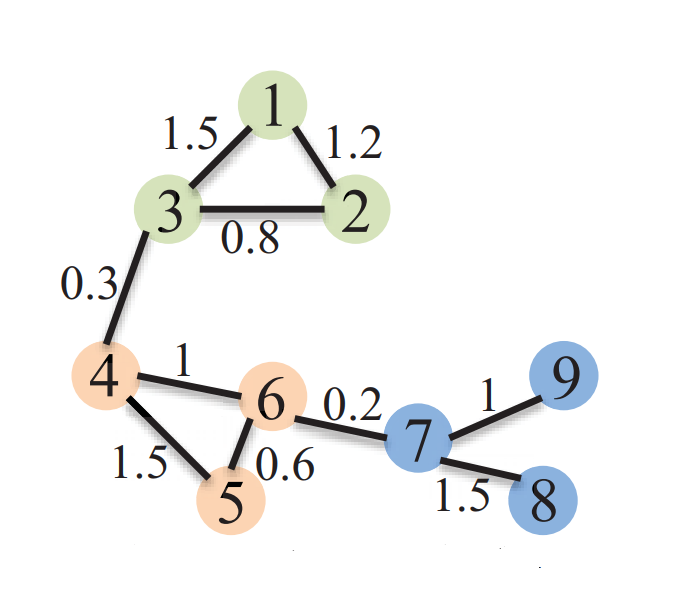
\includegraphics[width=7 cm]{images/graph_emb_1.png}
	\caption{Ví dụ về đồ thị đầu vào}
	\label{fig:graphInput}
\end{figure}

\begin{itemize}
	\item \begin{definition}[Đồ thị]\label{def:defGraph}
		\(\mathcal{G} = (V, E)\), trong đó \(v \in V\) là một đỉnh và \(e \in E\) là một cạnh. \(\mathcal{G}\) được liên kết với hàm ánh xạ loại đỉnh \(f_v: V \to T^v\) và hàm ánh xạ loại cạnh: \(f_e: E \to T^e\) .
	\end{definition}
	
	Trong đó: \(T^v\) và \(T^e\) lần lượt là tập hợp các loại đỉnh và loại cạnh. Mỗi đỉnh \(v_i \in V\) thuộc về một loại cụ thể, tức là, \(f_v(v_i) \in T^v\). Tương tự, đối với \(e_{ij} \in E, f_e (e_{ij}) \in T^e\).
	
	\item
	\begin{definition}[Đồ thị đồng nhất]\label{def:homogeneous}
		Đồ thị đồng nhất (homogeneous graph) : \textit{ $\mathcal{G}_{homo} = (V, E)$ là đồ thị trong đó $\mid T^v \mid = \mid T^e \mid = 1$. Tất cả các đỉnh trong $\mathcal{G}$ thuộc về một loại duy nhất và tất cả các cạnh thuộc về một loại duy nhất}.
	\end{definition}
	
	\item
	\begin{definition}[Đồ thị không đồng nhất]\label{def:heterogeneous}
		Đồ thị không đồng nhất (heterogeneous graph) : \textit{$\mathcal{G}_{hete} = (V, E)$ là một đồ thị trong đó $\mid T^v \mid > 1$ hoặc $\mid T^e \mid > 1$. Tức là có nhiều hơn một loại đỉnh hoặc nhiều hơn một loại cạnh}.
	\end{definition}
	
	\item
	\begin{definition}[Đồ thị tri thức]\label{def:knowledgeGraph}
		Đồ thị tri thức (knowledge graph)
		$\mathcal{G}_{know} = (V, R, E)$ là một đồ thị có hướng, có tập đỉnh là biểu diễn cho các thực thể (entities), tập quan hệ biểu diễn các mối quan hệ (relations) giữa các đỉnh, tập cạnh (edges) biểu diễn các sự kiện $E \subseteq V\times R \times V$ là gồm bộ ba subject-property-object. Mỗi cạnh là một mẫu gồm $(\text{entity}_{\text{head}}, \text{relation}, \text{entity}_{\text{tail}})$ (ký hiệu là $\langle h, r, t \rangle$) biểu thị mối quan hệ của $r$ từ thực thể $h$ đến thực thể $t$ .
	\end{definition}
	Trong đó $h, t \in V$ là các thực thể và $r \in R$ là các quan hệ. Chúng ta gọi $\langle h, r, t \rangle$ một bộ ba (triples) đồ thị tri thức.
	
	Ví dụ: trong hình \ref{fig:graphExample} có hai bộ ba: $\langle \text{Tom\ Cruise,\ born_in,\ New\ York} \rangle$ và $\langle \text{New York, state_of, U.S} \rangle$. Lưu ý rằng các thực thể và quan hệ trong đồ thị tri thức thường có các loại khác nhau. Do đó, đồ thị tri thức có thể được xem như là một ví dụ của đồ thị không đồng nhất.
\end{itemize}

\section{Dự đoán liên kết trong đồ thị tri thức}

Dự đoán liên kết (link prediction) hay hoàn thiện đồ thị tri thức (knowledge graph completion) là nhiệm vụ khai thác những sự kiện có sẵn trong đồ thị tri thức để suy luận ra sự kiện còn thiếu. Điều này tương đương với việc đoán đúng thực thể đuôi $\langle h, r, ? \rangle$ (dự đoán đuôi) hoặc $\langle ?, r, t \rangle$ (dự đoán đầu). Để đơn giản,  thay vì gọi dự đoán đầu hoặc đuôi, một cách tổng quát chúng ta gọi thực thể nguồn (source) là thực thể đã biết trong việc dự đoán, thực thể đích (target) là cái chúng ta cần dự đoán.


Hầu hết các nghiên cứu hiện tại về việc dự đoán liên kết của đồ thị tri thức đều liên quan đến các phương pháp tiếp cận tập trung vào khái niệm nhúng một đồ thị đã cho trong một không gian vectơ có số chiều thấp. Ngược lại với các tiếp cận này là một phương pháp đựa trên luật được nghiên cứu trong \cite{burl}. Thuật toán cốt lõi của nó dựa trên lấy mẫu một luật bất kỳ, sau đó khái quát  thành các quy tắc Horn\cite{wiki:Horn}. Tiếp đó dùng thống kê để tính độ tin cậy của các luật được khái quát. Khi dự đoán một liên kết mới (cạnh mới) của đồ thị chúng ta dự đoán một đỉnh có cạnh nối với một quan hệ cụ thể (label) với đỉnh còn lại hay không. Cũng đã có rất nhiều phương pháp được nghiên cứu, đề xuất để học các các luật trong đồ thị chẳng hạn như trong  RuDiK\cite{ortona2018robust}, AMIE\cite{galarraga2015fast}, RuleN\cite{meilicke2018fine}. 
Như đã nói trong phần trước có hai cách tiếp cận chính cho bài toán này một là tối ưu hóa hàm mục tiêu. Tìm ra một bộ quy tắc nhỏ bao gồm phần lớn các ví dụ là đúng và ít sai sót nhất có thể như được ngiên cứu trong RuDiK\cite{ortona2018robust}. Còn cách tiếp cận còn lại cũng là cách tiếp cận mà chúng tôi chọn nghiên cứu là cố gắng tìm hiểu mọi quy tắc khả thi có thể sau đó tạo xếp hạng \(k\) ứng viên tiềm năng với một độ tin cậy nhất định được đo trên tập huấn luyện.

Phương pháp đựa trên luật của chúng tôi phần lớn dựa vào phương pháp Anytime Bottom-Up Rule Learning for Knowledge Graph Completion \cite{meilicke2019anytime} mà sau đây chúng tôi gọi là \textbf{AnyBURL}. Như tên của phương pháp này phương pháp chủ yếu chú trọng vào vấn đề hoàn thành đồ thị, điền những phần còn thiếu vào đồ thị. Vấn đề tồn đọng lại ở mô hình này khi có một cạnh mới hay một tri thức mới được thêm vào đồ thị sẽ phải đào tạo lại toàn bộ mô hình. Chúng tôi giải quyết vẫn đề này theo hai chiến lược offline-to-online tức là khi thêm vào đồ thị tập hợp các cạnh thì mới thực hiện lại quá trình đào tạo lại một phần của đồ thị và chiến lược thứ 2 là online-to-online  khi thêm một cạnh mới sẽ thực hiện đào tạo lại ngay một phần có liên quan tới cạnh vừa thêm vào.

% GAT
Trong nhánh các phương pháp về học sâu, rất nhiều kỹ thuật học sâu thành công trong xử lý ảnh và xử lý ngôn ngữ tự nhiên được áp dụng vào đồ thị tri thức như : Mạng Neural Tích Chập (Convolution Neural Network - CNN \cite{lecun1999object}), Mạng Neural Hồi Quy (Recurrent Neural Network\cite{hopfield2007hopfield}), và gần đây như Transformer (\cite{yang2019xlnet}), Mạng Neural Bao Bọc (Capsule Neural Network - CapsNet \cite{sabour2017dynamic}). Bên cạnh đó các nghiên cứu còn sử dụng một số kỹ thuật khác như Random Walks, các mô hình dựa trên cấu trúc phân cấp, .. Ưu điểm chung của nhóm các phương pháp học sâu trên đồ thị tri thức đó là tự động rút trích các đặc trưng và có thể khái quát hóa cấu trúc phức tạp của đồ thị dựa trên một lượng lớn dữ liệu huấn luyện. Tuy nhiên, một số phương pháp chỉ chủ yếu tập trung vào cấu trúc dạng lưới mà không giữ được đặc trưng không gian của đồ thị tri thức. 
Cơ chế chú ý hay lớp chú ý đa đỉnh (multi-head attention layer) đã được áp dụng vào đồ thị bằng mô hình Mạng Đồ Thị Chú Ý (Graph Attention Network - GAT \cite{velivckovic2017graph}) giúp tổng hợp thông tin của một thực thể dựa vào trọng số chú ý của thực thể gốc đối với các thực thể lân cận. Tuy nhiên, mô hình đồ thị chú ý lại thiếu thông tin của vector nhúng quan hệ cũng như các vector nhúng lân cận của một thực thể gốc, một phần rất quan trọng giúp thể hiện vai trò của từng thực thể. Vấn đề đó đã được giải quyết trong báo cáo Learning Attention-based Embeddings for Relation Prediction in
Knowledge Graphs (\textbf{KBAT} \cite{nathani2019learning}), mô hình được chúng tôi chọn làm cơ sở nghiên cứu.
Cơ chế chú ý đang là một trong những cấu trúc học sâu đạt được hiệu quả nhất hiện nay (state-of-the-art) vì nó đã được chứng minh là thay thế cho bất kỳ phương pháp tính tích chập nào \cite{cordonnier2019relationship},
hơn nữa nó cũng nằm trong cấu trúc cơ bản để áp dụng trên các mô hình mới nhất trên ngôn ngữ tự nhiên như mô hình Megatron-LM \cite{shoeybi2019megatron}, và trên phân đoạn hình ảnh như mô hình HRNet-OCR (Hierarchical Multi-Scale Attention \cite{tao2020hierarchical}). Một số phương pháp thú vị \cite{cordonnier2020multi} đã cải tiến dựa trên cơ chế chú ý, tuy nhiên nó lại chưa được áp dụng vào đồ thị tri thức, vì vậy chúng tôi chọn nhóm phương pháp này để áp dụng các cải tiến mới nhất vào đồ thị tri thức.

\section{Các lĩnh vực nghiên cứu về đồ thị tri thức}

\begin{figure}[htp]
	\centering
	\tikzset{
		category/.style  = {draw, font=\sffamily, thin, align=center},
		subcat/.style={rectangle, rounded corners=6pt},
		center/.style = {category, ellipse, fill=blue!60, text width=4em},
		group/.style = {category, subcat, fill=blue!30, rounded corners=6pt, text width=6em},
		yellowbox/.style = {category, subcat, fill=yellow!30},
		greenbox/.style = {category, subcat, fill=green!30},
		redbox/.style = {category, subcat, fill=red!30},
		bluebox/.style = {category, subcat, fill=cyan!30},
		leafbox/.style = {category, subcat, fill=black!10, rounded corners=0mm}
	}
	\resizebox{\textwidth}{!}{%
		\begin{tikzpicture}
			\node[center] (root) {Đồ thị tri thức};
			\node[group][above left=1cm of root] (c1) {Học biểu diễn tri thức};
			\node[group][above right=8mm of root] (c2) {Nhận biết tri thức};
			\node[group][below left=5mm of root] (c3) {Thu nhận tri thức};
			\node[group][below right=20mm of root, xshift=-2cm] (c4) {Đồ thị tri thức thời gian};
			
			\begin{scope}[every node/.style={yellowbox}]
				\node[above=8mm of c1, xshift=-1cm] (c11) {Biểu diễn không gian};
				\node[left=of c1, yshift=9mm, xshift=-10mm] (c12) {Hàm đánh giá};
				\node[left=15mm of c1, yshift=-5mm] (c13) {Mã hóa mô hình};
				\node[left=of c1, yshift=-20mm] (c14) {Thông tin tương tự};
			\end{scope}
			
			\begin{scope}[every node/.style={redbox}]
				\node[above left=of c2, text width=35mm, yshift=1mm, xshift=18mm] (c21) {Hiểu ngôn ngữ tự nhiên};
				\node[above=1cm of c2, yshift=5mm, xshift=13mm] (c22) {Trả lời câu hỏi};
				\node[right=of c2, yshift=15mm] (c23) {Hệ thống hội thoại};
				\node[right=of c2, yshift=-2mm] (c24) {Hệ thống gợi ý};
				\node[below=5mm of c2, xshift=5mm] (c25) {Ứng dụng khác};
			\end{scope}
			
			\begin{scope}[every node/.style={greenbox}]
				\node[left=1cm of c3, yshift=5mm] (c31) {Khai phá thực thể};
				\node[below left=of c3, yshift=1cm, xshift=3mm] (c32) {Rút trích quan hệ};
				\node[below right=5mm of c3, xshift=-4cm] (c33) {Hoàn thiện đồ thị};
			\end{scope}
			
			\begin{scope}[every node/.style={bluebox}]
				\node[below=of c4, xshift=-15mm, yshift=-35mm] (c41) {Lý giải logic thời gian};
				\node[below=of c4, xshift=2cm, yshift=-23mm] (c42) {Quan hệ thời gian độc lập};
				\node[below right=of c4,xshift=-2mm, yshift=-10mm] (c43) {Thực thể động};
				\node[right=of c4, yshift=-2cm, xshift=15mm] (c44) {Nhúng thời gian};
			\end{scope}
			
			\begin{scope}[every node/.style={leafbox}]
				\node[above=5mm of c11] (c11x) {
					\begin{tabular}{@{}l@{}@{}l@{}}
						-Point-wise & -Đa tạp \\
						-Số phức & -Gausian \\
						-Rời rạc & \\
					\end{tabular}
				};
				\node[above=5mm of c12, xshift=-5mm] (c12x) {
					\begin{tabular}{@{}l@{}}
						-Khoảng cách \\
						-Ngữ nghĩa \\
						-Khác \\
					\end{tabular}
				};
				\node[left=of c13, yshift=5mm] (c13x) {
					\begin{tabular}{@{}l@{}}
						-Tuyến tính/ \\song tuyến tính \\
						-Ma trận hóa \\
						-Neural Nets \\
						-CNN \\
						-RNN \\
						-Transformers \\
						-GCN \\
					\end{tabular}
				};
				\node[below left=5mm of c14, xshift=6mm, yshift=-7mm] (c14x) {
					\begin{tabular}{@{}l@{}c@{}l@{}}
						-Văn bản & -Kiểu & -Trực quan \\
					\end{tabular}
				};
				%%%%%%%%%%%% 
				\node[below left=of c31] (c31x) {
					\begin{tabular}{@{}l@{}}
						-Nhận dạng \\
						-Định kiểu \\
						-Phân biệt \\
						-Sắp xếp \\
					\end{tabular}
				};
				\node[below=of c32, xshift=-5mm] (c32x) {
					\begin{tabular}{@{}l@{}}
						-Neural Nets\\
						-Chú ý \\
						-GCN \\
						-GAN \\
						-RL \\
						-Khác \\
					\end{tabular}
				};
				\node[below=5mm of c33] (c33x) {
					\begin{tabular}{@{}l@{}}
						-Nhúng dựa trên xếp hạng\\
						-Lý giải đựa trên đoạn \\
						-Lý giải dựa trên luật \\
						-Học siêu quan hệ \\
						-Phân loại bộ ba \\
					\end{tabular}
				};
				%%%%%%%%%%%%%%%%%
				\node[above=5mm of c22] (c22x) {
					\begin{tabular}{@{}l@{}}
						-Single-fact QA\\
						-Lý giải nhiều bước \\
					\end{tabular}
				};
				\node[below right=5mm of c25, yshift=15mm] (c25x) {
					\begin{tabular}{@{}l@{}}
						-Sinh câu hỏi\\
						-Công cụ tìm kiếm \\
						-Ứng dụng y khoa \\
						-Hồi phục sức khỏe \\
						-Phân loại ảnh zero-shot\\
						-Sinh văn bản\\
						-Phân tích ngữ nghĩa\\
					\end{tabular}
				};
				
			\end{scope}
			
			\foreach \value in {1,...,4}
			\draw[->, line width=0.8mm] (root) -> (c\value);
			
			\foreach \value in {1,...,4}
			\draw[->, ultra thick] (c1) -> (c1\value);
			\foreach \value in {1,...,4}
			\draw[->, thick] (c1\value) -> (c1\value x);
			
			\foreach \value in {1,...,5}
			\draw[->, ultra thick] (c2) -> (c2\value);
			\foreach \value in {2,5}
			\draw[->, thick] (c2\value) -> (c2\value x);
			
			\foreach \value in {1,...,3}
			\draw[->, ultra thick] (c3) -> (c3\value);
			\foreach \value in {1,...,3}
			\draw[->, ultra thick] (c3\value) -> (c3\value x);
			
			\foreach \value in {1,...,4}
			\draw[->, ultra thick] (c4) -> (c4\value);
			
	\end{tikzpicture}}
	\caption{
		Danh mục các lĩnh vực nghiên cứu trên đồ thị tri thức}
	\label{fig:categoriesResearch}
\end{figure}

Biểu diễn tri thức đã từng có lịch sử phát triển suốt chiều dài lịch sử trong lĩnh vực logic và trí tuệ nhân tạo. Trên đồ thị tri thức, có 4 bốn nhóm nghiên cứu chính đã được phân loại và tổng hợp ở báo cáo \cite{ji2020survey} bao gồm : Học Biểu Diễn Tri Thức (Knowledge Representation Learning), Thu Nhận Tri Thức (Knowledge Acquisition), Đồ Thị Tri Thức Về Thời Gian (Temporal Knowledge Graphs), Ứng Dụng Nhận Biết Tri Thức (Knowledge-aware Applications). Tất cả các danh mục nghiên cứu được minh họa ở hình \ref{fig:categoriesResearch}.

\textbf{Học biểu diễn tri thức}

Học biểu diễn tri thức là vấn đề tìm hiểu thiết yếu của đồ thị tri thức giúp mở ra rất nhiều ứng dụng trong thực tế. Học biểu diễn tri thức được phân loại thành bốn nhóm con bao gồm : 

\begin{itemize}
	\item \textit{Biểu Diễn Không Gian} (Representation Space) nghiên cứu về cách các thực thể và quan hệ được biểu diễn trong không gian. Biểu diễn không gian bao gồm không gian điểm (point-wise), đa tạp (manifold), không gian vector số phức (complex), phân phối Gaussian và không gian rời rạc.
	
	\item \textit{Hàm Đánh Giá} (Scoring Function) nghiên cứu về hàm đo lường giá trị của một bộ ba trong thực tế, bao gồm các hàm đánh giá dựa trên khoảng cách hoặc dựa trên sự tương đồng.
	
	\item \textit{Mã Hóa Mô Hình} (Encoding Models) nghiên cứu về cách biểu diễn và học các tương tác giữa các mối quan hệ. Đây là hướng nghiên cứu chính hiện nay, bao gồm các mô hình tuyến tính hoặc phi tuyến tính, phân rã ma trận hoặc mạng neural.
	
	\item \textit{Thông Tin Bổ Trợ} (Auxiliary Information) nghiên cứu về cách kết hợp vào các phương pháp nhúng, các thông tin bổ trợ bao gồm văn bản, hình ảnh và loại thông tin .
\end{itemize}

\textbf{Thu nhận tri thức}

Thu nhận tri thức nghiên cứu về cách thu nhận tri thức dựa trên đồ thị tri thức, bao gồm hoàn thiện đồ thị (knowledge graph completion), khai thác quan hệ và khai phá thực thể. Khai thác quan hệ và khai phát thực thể là nhóm phương pháp khai thác tri thức mới (bao gồm các quan hệ hoặc thực thể) trong đồ thị từ văn bản. Hoàn thiện đồ thị là nhiệm vụ mở rộng đồ thị tri thức dựa trên đồ thị đang có. Hoàn thiện đồ thị bao gồm các hướng nghiên cứu như : xếp hạng dựa trên nhúng (embedding-based ranking), dự đoán đường đi quan hệ (relation path reasoning), dự đoán dựa trên luật (rule-based reasoning) và học siêu quan hệ.
Khai phá thực thể bao gồm nhận dạng, phân biệt, định kiểu và sắp xếp. 
Các mô hình khai thác quan hệ sử dụng cơ chế chú ý, mạng đồ thị tích chập (graph
convolutional networks), huấn luyện đối nghịch (adversarial training), học tăng cường (reinforcement learning), học sâu và học chuyển tiến (transfer learning), đây là hướng nghiên cứu trong phương pháp đề xuất của chúng tôi.

Ngoài ra, trên đồ thị tri thức còn có các hướng nghiên cứu như \textbf{đồ thị tri thức về thời gian} và \textbf{ứng dụng nhận biết tri thức}. Đồ thị tri thức về thời gian sẽ kết hợp thêm thông tin thời gian trên đồ thị để học cách biểu diễn, còn ứng dụng nhận biết tri thức bao gồm hiểu ngôn ngữ tự nhiên (natural language understanding), trả lời câu hỏi (question answering), hệ thống gợi ý (recommendation systems) và nhiều nhiệm vụ khác trong thế giới thực mà nó tích hợp tri thức vào để cải thiện quá trình học biểu diễn .
% \chapter{Phương pháp dựa trên luật}
\label{Chapter2}

\section{Giới Thiệu}

Hiện nay các bài toán liên quan đến dự đoán liên kết đồ thị tri thức lớn rất được quan tâm có khoảng bốn nhánh nghiên cứu chính như được nhắc đến trong nghiên cứu \cite{ampligraph} một trong số đó là phương pháp dựa trên luật logic. Với mong muốn được tiếp cận các phương pháp từ đơn giản đến phức tạp nên chúng tôi chọn phương pháp này làm chủ để chính cho các báo cáo và nghiên cứu trong chương này. Với phương pháp này đưa ra một xếp hạng \(k\) ứng viên với một số điểm nhất định biểu thị cho sự chắc chán của dự đoán nó phù hợp với các hệ thống gợi ý(recommender system).

\section{Các công trình liên quan}
Hầu hết các nghiên cứu hiện tại về việc dự đoán liên kết của đồ thị tri thức đều liên quan đến các phương pháp tiếp cận tập trung vào khái niệm nhúng một đồ thị đã cho trong một không gian vectơ có số chiều thấp. Ngược lại với các tiếp cận này là một phương pháp đựa trên luật được nghiên cứu trong \cite{burl}.Thuật toán cốt lõi của nó dựa trên lấy mẫu một luật bất kỳ, sau đó khái quát  thành các quy tắc Horn\cite{wiki:Horn} Tiếp đó dùng thống kê để tính độ tin cậy của các luật được khái quát. Khi dự đoán một liên kết mới (cạnh mới) của đồ thị chúng ta dự đoán một đỉnh có cạnh nối với một quan hệ cụ thể (label) với đỉnh còn lại hay không.Cũng đã có rất nhiều phương pháp được nghiên cứu, đề xuất để học các các luật trong đồ thị chẳng hạn như trong   RuDiK \cite{dettmers2018convolutional}, AMIE\cite{galarraga2015fast}, RuleN\cite{meilicke2018fine}. Trong phương pháp RuDiK học các luật có thể học cả quy tắc positive và negative. Trong khi phương pháp của chúng tôi chỉ học các quy tắc positive. RuDiK tìm ra một bộ quy tắc nhỏ bao gồm phần lớn các ví dụ là đúng và ít sai sót nhất có thể. Điều này khác với mục tiêu của chúng tôi, chúng tôi cố gắng tìm hiểu mọi quy tắc khả thi có thể sau đó tạo xếp hạng \(k\) ứng viên tiềm năng với một độ tin cậy nhất định đuọc đo trên tập huấn luyện.

Phương pháp của chúng tôi phần lớn dựa vào phương pháp Anytime Bottom-Up Rule Learning for Knowledge Graph Completion \cite{meilicke2019anytime} mà sau đây chúng tôi gọi là \textbf{AnyBURL}. Vấn đề tồn đọng lại ở mô hình này khi có một cạnh mới hay một tri thức mới được thêm vào đồ thị sẽ phải đào tạo lại toàn bộ mô hình. Chúng tôi giải quyết vẫn đề này theo hai chiến lược offline-to-online tức là khi thêm vào đồ thị tập hợp các cạnh thì mới thực hiện lại quá trình đào tạo lại một phần của đồ thị và chiến lược thứ 2 là online-to-online  khi thêm một cạnh mới sẽ thực hiện đào tạo lại ngay một phần có liên quan tới cạnh vừa thêm vào.
\section{Phương pháp đề xuất}
Trong phần này chúng tôi mô tả lại cách mô hình hóa lại bài toán theo phương pháp dựa trên luật AnyBURL,thuật toán lấy mẫu luật (đường đẫn) và thuật toán khái quát hóa một luật để lưu trữ trở thành tri thức của mô hình. Cùng với những cải tiến của chúng tôi trong quá trình đào tạo khi có một tri thức mới được thêm vào đồ thị(thêm cạnh).
\subsection{Horn rule}
Trong logic toán học, một công thức nguyên tử - \textbf{atomic formula}\cite{wiki:Atomic} (còn được gọi đơn giản là một nguyên tử-\textbf{atom}) là một công thức không có cấu trúc mệnh đề, nghĩa là một công thức không chứa các liên kết logic (\(\vee, ~ \wedge\)) hoặc tương đương (\(\Leftrightarrow\)) là một công thức không có các mẫu con nghiêm ngặt (tức là atom không thể chia nhỏ ra thành các atom con nữa). Do đó, các nguyên tử là công thức đơn giản nhất để hình thành luật của logic. Các công thức hợp được hình thành bằng cách kết hợp các công thức nguyên tử bằng cách sử dụng các liên kết logic.

Một \textbf{literal}\cite{wiki:Literal} là một công thức nguyên tử (nguyên tử) hoặc phủ định của nó. Định nghĩa chủ yếu xuất hiện trong lý thuyết logic cổ điển. \textbf{Literal} có thể được chia thành hai loại: Một \textbf{positive literal} chỉ là một nguyên tử (ví dụ: \(x\)). Một \textbf{negative literal} là phủ định của một nguyên tử (ví dụ: \(\neg x\)). Sự phân chia của \textbf{literal} là \textbf{positive literal} hay \textbf{negative literal} tùy thuộc vào việc \textbf{literal} được định nghĩa.

Một mệnh đề (clause) là một literal hoặc nối rời của hai hoặc nhiều literal. Ở dạng \textbf{Horn} một mệnh đề có nhiều nhất một positive literal. Lưu ý: Không phải mọi công thức trong logic mệnh đề đều có thể đưa về dạng Horn.Mệnh đề xác định không có literal đôi khi được gọi là mệnh đề đơn vị (unit clause) và một mệnh đề đơn vị không có biến đôi khi được gọi là \textit{facts}\cite{wiki:Horn}.Một công thức nguyên tử được gọi là \textit{ground} hoặc \textit{ground atoms} nếu nó được xây dựng hoàn toàn từ các mệnh đề đơn vị; tất cả các \textit{ground atoms} có thể ghép lại từ một tập hợp hàm và các ký hiệu vị từ nhất định tạo nên cơ sở Herbrand cho các bộ ký hiệu này\cite{wiki:Term}.

\subsection{Định nghĩa đồ thị  tri thức} \label{kg}
Một đồ thị tri thức \(\mathbb{G}\) được định nghĩa trên một bộ từ vựng \(\langle \mathbb{C}, \mathbb{R} \rangle\) trong đó \(\mathbb{C}\) là tập hợp các hằng số và \(\mathbb{R}\) là tập hợp các vị từ nhị phân.Khi đó, \(\mathbb{G} = \{r (a, b) \mid r \in \mathbb{R}, a, b \in \mathbb{C}\}\) là tập hợp các \textit{ground atoms} hoặc \textit{facts}. Một vị từ nhị phân được gọi là quan hệ và hằng số (hoặc hằng số được đề cập đến) được gọi là thực thể (entity) tương ứng với một dòng dữ liệu trong tập huấn luyện. Sau đây chúng tôi sử dụng các chữ cái viết thường cho các hằng và chữ in hoa cho các biến cho các thảo luận dưới đây. Vì chúng ta không học các quy tắc Horn tùy ý, và chỉ học đối với loại quy tắc nào có thể được khái quát hóa như được thảo luận dưới đây.

Chúng ta định nghĩa một quy tắc là \(h(c_0, c_n) \gets b_1(c_0, c_1) ,\dots ,b_n(c_{n}, c_{n + 1})\) là một đường dẫn ground atoms có chiều dài \(n\). Trong đó \(h(\dots)\) được gọi là \textit{head atoms} và \( b_1(c_0, c_1) ,\dots ,b_n(c_{n}, c_{n + 1})\) được gọi là \textit{body atoms}. Chúng tôi sẽ phân biệt dưới đây ba loại quy tắc mà chúng tôi gọi là: \textit{quy tắc nhị phân} \((\mathbf{B})\) là quy tắc trong head atoms chứa 2 biến, quy tắc đơn nguyên kết thúc bằng một đỉnh treo  và atom này chỉ chứa biến không chứa hằng số\((\mathbf{U_d})\) và head atoms chỉ chứa 1 biến. Còn quy tắc đơn nguyên kết thúc bằng một atom \((\mathbf{U_c)}\) và head atoms cũng chỉ chứa 1 biến.\((\mathbf{U_c)}\)  có thể là một đỉnh treo tới một hằng số bất kì nếu hằng số này trùng mới hằng số trong head atom thì tạo thành một đường đẫn có chu trình.

\[B \hspace{3.7cm} h(A_0,A_n) \gets  \bigwedge^n_{i=1} b_i(A_{i-1}, A_i)\]
\[U_d \hspace{3.8cm} h(A_0,c) \gets  \bigwedge^n_{i=1} b_i(A_{i-1}, A_i)\]
\[U_c \hspace{1cm} h(A_0,c) \gets  \bigwedge^{n-1}_{i=1} b_i(A_{i-1}, A_i) \wedge b_n(A_{n-1}, c^{\prime})\]

Chúng tôi gọi các quy tắc của các loại này là quy tắc đường đi (path rules), bởi vì các body atoms (phần sau đấu \(\gets\)) tạo thành một đường đi. Lưu ý rằng nó cũng bao gồm các biến thể quy tắc với các biến được đảo ngược trong các nguyên tử: được đưa ra trong đồ thị tri thức \(\mathbb{G}\), đường dẫn có độ dài \(n\) là một chuỗi gồm \(n\) bộ ba \(p_i (c_i, c_i + 1)\) với \(p_i (c_i, c_i + 1) \in \mathbb{G}\) hoặc \(p_i (c_i + 1, c_i) \in \mathbb{G}\) với \(0 \geq i \leq n\). Các mẫu quy tắc trừu tượng (abstract rule patterns) được cho ở trên có độ dài \(n\) vì body atoms của chúng có thể được khởi tạo thành một đường dẫn có độ dài \(n\).

Ngoài ra Quy tắc \(B\) và quy tắc \(U_c\) cũng được gọi là quy tắc kết nối kín. Chúng có thể được học bởi hệ thống khai thác AMIE được mô tả trong \cite{AMIE,galarraga2015fast}. Quy tắc \(U_d\) là quy tắc không đóng hay đường đi không tạo thành chu trình vì \(A_n\) là biến chỉ xuất hiện một lần. Ví dụ:
\[
\begin{matrix}
\textit{speaks}(X, Y ) & \gets & \textit{lives}(X, Y) & \quad (1) \\
\textit{lives\_in\_city}(X, Y ) & \gets & \textit{lives}(X, A),\textit{within}(Y, A)  & \quad  (2) \\
\textit{gen}(X, female) & \gets & \textit{married}(X, A), \textit{gen}(A, male)  & \quad  (3) \\
\textit{profession}(X, actor) &  \gets & \textit{acted\_in}(X, A)  & \quad (4)
\end{matrix}
\]
Quy tắc (1) là quy tắc \textbf{B}(quy tắc nhị phân) quy tắc này nói rằng nếu một người (thực thể) \(X\) nói nguôn ngữ \(Y\) nếu người \(X\) sống  ở đất nước \(Y\).Rõ ràng quy tắc này là một quy tắc khái quát miễn khi nào thực thể \(X\) có cạnh nối với thực thể \(Y\) với nhãn là \textit{lives} thì có thể kết thêm 1 cạnh với nhãn \textit{speaks} giữa \(X\) và \(Y\). Quy tắc (2), (3) điều là quy tắc \(U_c\) ,quy tắc (2) nói rằng người \(X\) sống ở thành phố \(Y\) nếu người \(X\) sống ở quốc gia \(A\) và thành phố \(Y\) nằm trong quốc gia \(A\), quy tắc (3) nói rằng nếu một người \(X\) là nữ nếu họ kết hôn với một người \(A\) và người \(A\) có giới tính nam. Ở quy tắc (3) không tạo thành chu trình trên đồ thị như quy tắc (2) đỉnh (Y) lặp lại  ở \textit{head atom} và đỉnh cuối cùng trong \textit{body atoms}. Quy tắc (4) là quy tắc \(U_d\) nói rằng người \(X\) là một điễn viên nếu người \(X\) đóng trong một bộ phim \(A\).

Tất cả các quy tắc được xem xét sẽ được lọc lại đựa trên điểm được gọi là độ tin cậy của quy tắc là được đo trên tập dữ liệu huấn luyện. Độ tin cậy này được đo bằng tỷ lệ body atoms dẫn đến head atoms chia cho tất cả các đường đãn chứa body atoms.Ví dụ khi ta có quy tắc sau:
\(\textit{gen}(X, female) \gets \textit{married}(X, A), \textit{gen}(A, male) \). Khi đó chúng ta thực hiện đếm tất cả các cặp thực thể có quan hệ  \(\textit{married}(X, A), \textit{gen}(A, male) \) được gọi là số đường dẫn chứa body atoms, sau đó thực hiện đếm tất cả các  thực thể thỏa quan hệ \(\textit{gen}(X, female) \gets \textit{married}(X, A), \textit{gen}(A, male) \) được gọi là số body atoms dẫn đến head atoms. Sau đó chia số body atoms dẫn đến head atoms cho  đường dẫn chứa body atoms được gọi là độ tin cậy của quy tắc.
\subsection{Thuật toán} \label{algorithm2}
Trong phần này chúng tôi mô tả lại thuật toán chính của phương pháp AnyBURL nó cũng được mô tả trong \cite{burl} cũng như hai thuật toán mở rộng của chúng tôi để giải quyết vấn đề khi đồ thị được thêm một hoặc một lượng tri thức mới (thêm cạnh). Ngoài ra chúng tôi cũng mô tả sơ lược lại cách khởi tạo một luật cũng như cách thức tính toán độ tin cậy bằng cách lấy mẫu trên tập huấn luyện và vấn đề độ tin cậy khi dự đoán một luật khi tính toán độ tin cậy bằng việc lấy mẫu.
\subsubsection{Thuật toán 1 AnyBURL}
\begin{algorithm}
\caption{Anytime Bottom-up Rule Learning}\label{euclid}
\begin{algorithmic}[1]
\Procedure{AnyBURL($\mathbb{G}$, s, sat, Q, ts)}{}
\State $\textit{n} = \text{2}$
\State $R = \emptyset$
\Loop
\State $R_s = \emptyset$
\State $start = currentTime()$
\Repeat
\State $p = samplePath(\mathbb{G}, n)$
\State $R_p = generateRules(p)$
\For {$r \in R_p$}
\State $score(r, s)$
\If {$Q(r)$}
	\State $R_s = R_s \cup \{r\}$
\EndIf
\EndFor
\Until {$currentTime() > start + ts$}
\State $R^{\prime}_s = R_s \cap R$
\If {$ \mid R^{\prime} \mid / \mid R \mid > SAT$}
	\State $n = n + 1$
\EndIf
\State $R = R_s \cap R$
\EndLoop
\Return R
\EndProcedure
\end{algorithmic}
\end{algorithm}

Đầu vào của thuật toán \(\mathbb{G}, S, SAT, Q, TS\). Đầu ra là tập hợp \(R\) các luật học được. Trong đó \(\mathbb{G}\) là một đồ thị tri thức được cho từ tập dữ liệu đào tạo. \(S\) là tham số cho biết kích thước của một lần lấy mẫu trên dữ liệu đào tạo để tính toán độ tin cậy. \(SAT\) cho biết độ bão hòa(saturation) của các luật được sinh ra trong 1 lần lặp độ bão hòa này được tính bằng số luật \textbf{mới} học được ở lần lặp hiện tại so số sô luật đã học được. Nếu nhỏ hơn độ bão hòa thì chúng tôi cho rằng vẫn còn tiềm năng để khai thác các luật với độ dài \(n\). ngược lại chúng tôi tăng độ dài của luật sau đó tiếp tục khai thác. \(Q\) là một ngưỡng để xác định xem luật mới được sinh ra có được thêm vào kết quả trả về hay không. Còn \(TS\) cho biết thời gian học của thuật toán. Chúng tôi bắt đầu với \(n\) bằng \(2\) tức là các luật có độ dài đường đẫn bằng 2 vì trong path rule yêu cầu ít nhất 1 literal trong head atom và 1 trong body atoms. Ở phần lấy mẫu 1 luật(\textit{samplePath}) chỉ đơn giản là chúng ta chọn 1 đỉnh bất kì trong đồ thị duyệt qua tất cả các đường đẫn từ đỉnh đó đi qua \(n\) đỉnh khác, sau đó chọn ngẫu nhiên 1 đường đẫn trong số các trường đẫn duyệt được.

\subsubsection{Thuật toán 2 tạo 1 luật}
\begin{algorithm}
\caption{Generate Rules(p)}\label{euclid}
\begin{algorithmic}[1]
\Procedure{generate\_rules(p)}{}
\State $\textit{generalizations} = \emptyset$
\State $is\_binary\_rule = random.choices([true,false])$
\If {$is\_binary\_rule$}
	\State $replace\_all\_head\_by\_variables(p)$
	\State $replace\_all\_tail\_by\_variables(p)$
	\State $add(generalizations, p)$
\Else:
    \State $replace\_all\_head\_by\_variables(p)$
    \State $add(generalizations, p)$
    \State $replace\_all\_tail\_by\_variables(p)$
	\State $add(generalizations, p)$
\EndIf
\Return $generalizations$
\EndProcedure
\end{algorithmic}
\end{algorithm}

Ở thuật toán này chúng tôi thay các hằng số vào các head và tail trong toàn bộ path rule  của luật được lấy mẫu ở bước trước nếu luật cần học là luật nhị phân ngược lại chúng tôi chỉ thay hoặc head hoặc tail rồi thêm vào luật trả về sau đó chúng tôi lấy mẫu trên tập huấn luyện 1 tập hợp các luật sau đó tính toán độ tin cây như được mô tả trong phần \hyperref[kg]{2.3.2}. Để giảm chi phí tính toán chúng tôi chọn cách lấy mẫu trên tập huấn luyện để tính toán. Khi đưa ra dự đoán các ứng cử viên của một luật chúng tôi sẽ tính toán lại bằng cách thêm vào một lượng biểu diẽn số luật bị sai mà chúng tôi chưa nhìn thấy trong quá trình lấy mẫu để tính toán độ tin cậy. Dối với mô hình của chúng thôi sau khi thử nghiệm tham số trong khoảng \([5, 10]\) cho kết quả tốt nhất.

\subsubsection{Thuật toán 3 học offline-to-online}
\begin{algorithm}
\caption{AnyBURL Learning batch size}\label{euclid}
\begin{algorithmic}[1]
\Procedure{AnyBURLbatch($\mathbb{G}$, s, sat, Q, ts, batch\_edge)}{}
\State $is\_connected = add(\mathbb{G}, batch\_edge)$
\If {$is\_connected$}
	\State  $ G^{\prime} = \mathbb{G} \oplus batch\_edge$
\Else
    \State  $ G^{\prime} = batch\_edge$
\EndIf
\State $\textit{n} = \text{2}$
\State $R = \emptyset$
\Loop
\State $R_s = \emptyset$
\State $start = currentTime()$
\Repeat
\State $p = samplePath(G^{\prime}, n)$
\State $R_p = generateRules(p)$
\For {$r \in R_p$}
\State $score(r, s)$
\If {$Q(r)$}
	\State $R_s = R_s \cup \{r\}$
\EndIf
\EndFor
\Until {$currentTime() > start + ts$}
\State $R^{\prime}_s = R_s \cap R$
\If {$ \mid R^{\prime} \mid / \mid R \mid > SAT$}
	\State $n = n + 1$
\EndIf
\State $R = R_s \cap R$
\EndLoop
\Return R
\EndProcedure
\end{algorithmic}
\end{algorithm}

Thuật toán này là phần bổ xung của chúng tôi để tránh việc phải đào tạo lại toàn bộ mô hình khi có một lượng tri thức mới được thêm vào đồ thị. Khi thêm vào đồ thị chúng tôi kiểm trả xem phần tri thức mới có kết nối với tri thức cũ hay không (tính liên thông) nếu có chúng tôi thực hiện phép toán \(\oplus\) lấy  tất cả các phần trong \(batch\_edge\) thêm với 1 phần liên thông với những cạnh liên thông với đồ thị với dộ dài là \(5\), Nếu không chúng tôi lấy tất cả các phần trong \(batch\_edge\) sau đó thực hiện lại các bước như thuật toán Anytime Bottom-up Rule Learning.

\subsubsection{Thuật toán 4 học online-to-online}
\begin{algorithm}
\caption{AnyBURL Learning batch size}\label{euclid}
\begin{algorithmic}[1]
\Procedure{AnyBURLbatch($\mathbb{G}$, s, sat, Q, ts, edge)}{}
\State $is\_connected = add(\mathbb{G}, edge)$
\State $R = \emptyset$
\If {$is\_connected$}
    \State $\textit{n} = \text{2}$
    \State $R_s = \emptyset$
    \Repeat
        \State $p = samplePath(edge, n)$
        \State $R_p = generateRules(p)$
        \For {$r \in R_p$}
            \State $score(r, s)$
            \If {$Q(r)$}
        	    \State $R_s = R_s \cup \{r\}$
            \EndIf
        \EndFor
    \Until {$currentTime() > start + ts$}
    \State $R^{\prime}_s = R_s \cap R$
    \If {$ \mid R^{\prime} \mid / \mid R \mid > SAT$}
    	\State $n = n + 1$
    \EndIf
    \State $R = R_s \cap R$
\State \Return R
\EndIf
\EndProcedure
\end{algorithmic}
\end{algorithm}

Thuật toán này là một phần bổ xung cho thuật toán 3 ở trên. Sở dĩ chúng tôi gọi là online-to-online là vì khi có một cạnh mới(tri thức mới) được thêm vào đồ thị chúng tôi sẽ thực hiện việc học ngay tức khắc trên các path rule liên quan tới cạnh đó không giống như ở thuật toán 3 khi có đủ 1 lượng tri thức mới được thêm vào.

% Nội dung báo cáo được phân thành các chương. Số thứ tự của các chương, mục được đánh số bằng hệ thống số Ả-rập, không dùng số La mã. Các mục và tiểu mục được đánh số bằng các nhóm hai hoặc ba chữ số, cách nhau một dấu chấm: số thứ nhất chỉ số chương, chỉ số thứ hai chỉ số mục, số thứ ba chỉ số tiểu mục.

% %Báo cáo cần dùng LaTEX để viết và trình bày theo mẫu đã được cung cấp.

%  Báo cáo trình bày sử dụng khổ giấy với việc canh lề như sau: Lề trên 3 cm, lề dưới 2,5 cm, lề trái 3 cm, lề phải 2 cm. Đánh số trang ở giữa bên dưới. Đánh số trang ở giữa bên dưới.

% Font chữ dùng trong báo cáo (Times New Roman) với kích cỡ (size) 13-14pt, sử dụng chế độ dãn dòng (line spacing) chế độ 1.5 lines.

%Các bảng biểu trình bày theo chiều ngang khổ giấy thì đầu bảng là lề trái của trang.

\section{Kết quả thí nghiệm}
Trong phần này chúng tôi mô tả lại các bộ dữ liệu mà chúng tôi đùng để thực nghiệm đánh giá phương pháp của chúng tôi cùng với so sánh với các kết quả khác của các công trình nổi bật khác được báo cáo trong \hyperref[tab:tab1]{bảng 2.1}. Ngoài ra chúng tôi cũng cố gắng đánh giá hai đề xuất của chúng tôi trong việc thêm một lượng tri thức mới vào đồ thị bằng cách chúng tôi xem tập test là một lượng tri thức mới cần thêm vào và dùng tập vadidation để đánh giá lại phương pháp của chúng tôi. Kết quả chi tiết được báo cáo ở \hyperref[tab:tab1]{bảng 2.2}
\subsection{Các tập dữ liệu huấn luyện} \label{datasets}
Trong thí nghiệm của chúng tôi, chúng tôi thực hiện trên bốn tập dữ liệu phổ biến là FB15k, FB15-237, WN18 và WN18RR.Các bộ dữ liệu này là tập hợp các bộ ba (triple) \(\langle head, relation, tail \rangle\) biểu thị cho thực thể đầu có một mối quan hệ với thực thể cuối.

Bộ dữ liệu FB15k: Bộ dữ liệu này được tạo bởi nhóm nghiên cứu A. Bordes, N. Usunier, A. Garcia-Duran, J. Weston, and O. Yakhnenko \cite{bordes2013translating} bằng cách trích xuất từ bộ dữ liệu Wikilinks database \footnote{https://code.google.com/archive/p/wiki-links/}.Wikilinks database thu thập các siêu liên kết(hyperlinks) đến Wikipedia gồm 40 triệu lượt đề cập trên 3 triệu thực thể, họ trích xuất tất cả các dữ kiện liên quan đến một thực thể nhất định có hơn 100 lần được đề cập đến bởi các tài liệu khác cùng với tất cả các dữ kiện liên quan đến thực thể đó (bao gồm cả những thực thể con được nhắc đến trong tài liệu Wikipedia đó), ngoại trừ những thonng tin như: ngày tháng, danh từ riêng, v.v ... Họ cũng chuyển đổi các đỉnh có bậc \(n\) được biểu diễn thành các nhóm các cạnh nhị phân tức là liệt kê các cạnh và quan hệ của mọi đỉnh. Tập dữ liệu được chia ngẫu nhiên thành 3 tập: tập training với 1345 relations, 14834 head entities và 14903 tail entities, tập test gồm 916 relations, 11886 head entities, và 11285 tail entities, tập vadiation gồm 961 relations, 12297 head entities, và 11825 tail entities.

Bộ dữ liệu FB15k-237: là một tập hợp con của FB15k được xây dựng bởi Toutanova và Chen \cite{toutanova2015observed} lấy cảm hứng từ quan sát rằng FB15k bao gồm dữ liệu thử nghiệm được các mô hình nhìn thấy tại thời điểm đào tạo(test leekage). Trong FB15k, vấn đề này là do sự hiện diện của các quan hệ gần giống nhau hoặc nghịch đảo của nhau.FB15k-237 được xây dựng để trở thành một tập dữ liệu thách thức hơn: các tác giả đã chọn các dữ kiện liên quan đến 401 quan hệ xuất hiện nhiều nhất và loại bỏ tất cả các quan hệ tương đương hoặc nghịch đảo. Họ cũng đảm bảo rằng không có thực thể nào được kết nối trong tập huấn luyện cũng được liên kết trực tiếp trong tập test và validation.Tập training gồm 237 relations, 13781 head entities, và 13379 tail entities, tập test gồm 223 relations, 7652 head entities, và 5804 tail entities, tập vadition gồm 224 relations, 8171 head entities, and 6376 tail entities.

Bộ dữ liệu WN18: được giới thiệu bởi các tác giả của TransE \cite{bordes2013translating}, được trích xuất từ WordNet\footnote{https://wordnet.princeton.edu/}, một bản thể học ngôn ngữ KG có nghĩa là cung cấp một từ điển/từ đồng nghĩa để hỗ trợ NLP và phân tích văn bản tự động. Trong WordNet, các thực thể tương ứng với các tập hợp (\textit{word senses}) và các quan hệ đại diện cho các kết nối từ vựng của chúng (ví dụ: “hypernym”). Để xây dựng WN18, các tác giả đã sử dụng WordNet làm điểm bắt đầu và sau đó lặp đi lặp lại lọc ra các thực thể và mối quan hệ với quá ít lần được đề cập. Tập dữ liệu được chia ngẫu nhiên thành 3 tập: tập training với 18 relations, 40504 head entities, và 40551 tail entities, tập test gồm 18 relations, 4262 head entities, and 4338 tail entities, tập vadiation gồm 18 relations, 4349 head entities, and 4263 tail entities.

Bộ dữ liệu WN18RR: là một tập hợp con của WN18 được xây dựng bởi DeŠmers et al.\cite{dettmers2017convolutional}, cũng là người giải quyết vấn đề rò rỉ thử nghiệm (test leakage)trong WN18. Để giải quyết vấn đề đó, họ xây dựng tập dữ liệu WN18RR thách thức hơn nhiều bằng cách áp dụng một phương pháp tương tự đưược sử dụng cho FB15k-237 \cite{toutanova2015observed}. Training gồm 11 relations, 39610 head entities, và 31881 tail entities, tập test gồm 11 relations, 2958 head entities, và 2619 tail entities, tập vadition gồm 11 relations, 2851 head entities, and 2575 tail entities.

\subsection{Kết quả thực nghiệm}
Trong phần này chúng tôi mô tả lại các phương pháp đánh giá(độ do), môi trường thực hiện cũng như các tập dữ liệu mà chúng tôi sử dụng để dánh giá phương pháp của mình. Các phương pháp đánh giá(độ do) này cũng phổ biến nó được đánh giá cho hầu hết các mô hình dự đoán liên kết trên đồ thị. Chúng tôi tiến hành so sánh với bốn phương pháp nổi bật khác được báo cáo trong \cite{rossi2020knowledge}.
\subsubsection{Các độ đo}
\textit{Mean Rank} (MR). Đây là giá trị trung bình của rank thu được cho một dự đoán chính xác. Càng nhỏ thì mô hình càng chính xác:
\[MR = \frac{1}{\mid Q \mid} \sum_{q ~\in~ Q} rank(q) \]
Trong đó \(\mid Q \mid\) là độ lớn của tập hợp các câu hỏi bằng độ lớn của tập test hoặc vadidation. Khi dự đoán chúng tôi dự đoán cả head và tail cho một dòng tương ứng trong tập dữ liệu thử nghiệm. Ví dụ chún tôi sẽ dự đoán \(\langle ?,~ relation,~ tail \rangle\) và \(\langle head,~ relation,~ ?\rangle\) cho 1 dòng tương ứng. \(q\) thể hiện cho câu hỏi chúng tôi dự đoán và \(rank(q)\) thể hiện cho kết quả đúng của câu hỏi đứng ở vị trí thứ mấy trong xếp hạng của chúng tôi sau đó lấy trung bình rank của các dự đoán head và tail. Rõ ràng độ đo này nằm giữa \([1, \mid \text{số lượng các entity} \mid]\) do có tối da \(n\) cạnh nối 1 đỉnh tới \(n-1\) đỉnh còn lại và thêm cạnh nối tới chính đỉnh nó(cạnh khuyên). Và độ đo này đễ bị ảnh hưởng bởi nhiễu vì có những quan hệ có những thực thể được xếp hạng gần cuối. Để giải quyết vấn đề này nhóm chúng tôi và các nhóm nghiên cứu khác sử dụng thêm độ đo Mean Reciprocal Rank (MMR).

\textit{Mean Reciprocal Rank} (MMR). Đây là xếp hạng đối ứng trung bình, là nghịch đảo của giá trị trung bình của rank thu được cho một dự đoán chính xác ở trên. Và càng lớn thì mô hình càng chính xác. Do độ đo này lấy nghịch đảo của các rank nên tránh dược vấn đề nhiễu của độ đo MR ở trên.
\[MRR =\frac{1}{\mid Q \mid} \sum_{q~ \in ~Q} \frac{1}{rank(q)}\]

\textit{Hit@K} (H@K). Đó là tỷ lệ các dự đoán đúng mà rank nhỏ hơn hoặc bằng ngưỡng \(K\):
\[H@K = \frac{\mid {q ~\in ~Q~: rank(q) \leq K} \mid}{\mid Q \mid}\]
\subsubsection{Kết quả}
Như đã nói trước đây với mô hình dựa trên luật của chúng tôi hoàn toàn có thể thực hiện trên một laptop với cấu hình thông thường. Trong thí nghiệm của chúng tôi cấu hình máy để thực thi như sau: T480, core i5 8th Gen, ram 16Gb, 4 core 8 thread. Mã nguồn thực thi được viết bằng ngôn ngữ Python phiên bản 3.6 và dùng các hàm hỗ trợ có sẵn trong Python với không một thư viện bên thứ ba nào. Thí nghiệm được thực hiện với bốn tập dữ liệu phổ biến là FB15k, FB15-237, WN18 và WN18RR. Thông tin chi tiết các bộ dữ liệu này được mô tả ở phần \hyperref[datasets]{các tập dữ liệu huấn luyện}.

Như mô tả ở phần \hyperref[algorithm2]{thuật toán AnyBURL} thuật toán này sẽ học các luật được sinh ra trong một khoảng thời gian nhất định do người dùng cấu hình. Ở đây chúng tôi chọn cấu hình thời gian là 1000 giây tương đương khoảng 17 phút đào tạo, với độ bão hòa(SAT) \(0.85\), độ tin cậy Q \(0.05\), kích thước mẫu S (\(\frac{1}{10}~ \text{tập huấn luyện}\)). Với cấu hình như vậy mô hình phiên bản Python của chúng tối cho kết quả tương đương với phiên bản Java nhóm tác giả Meilicke, Christian et al. \cite{burl} với cấu hình tương tự nhưng thời gian training là 100 giây. Sự khác biệt về thời gian học tập ở đây chủ yếu là do hiệu năng của hai ngôn ngữ Python và Java. Ở đây chúng tôi chọn ngôn ngữ Python vì nó được dùng làm ngôn ngữ chính cho nhiều mô hình trí tuệ nhân tạo gần đây, và cũng thuận tiện cho chúng tôi khi so sánh hiệu năng cũng như đánh giá với các phương pháp học sâu khác da số được viết bằng Python.

Bảng \hyperref[tab:tab1]{2.1} bên dưới mô tả các kết quả thực nghiệm của chúng tôi với các độ đo \(H@K\) cùng với các kết quả thực nghiệm của các phương pháp khác được đề cập trong khảo  sát \cite{rossi2020knowledge}

\begin{table}[ht]
\caption{Kết quả phương pháp AnyBURL}
\label{tab:tab1}%
\begin{center}
\resizebox{\textwidth}{!}{%
\begin{tabular}{lllllllllllllllll}
\cline{2-17}
\multicolumn{1}{l|}{} &
  \multicolumn{4}{c|}{\textbf{FB15k}} &
  \multicolumn{4}{c|}{\textbf{FB15-237}} &
  \multicolumn{4}{c|}{\textbf{WN18}} &
  \multicolumn{4}{c|}{\textbf{WN18RR}} \\ \cline{2-17}
\multicolumn{1}{l|}{} &
  \multicolumn{1}{l|}{\textbf{H@1}} &
  \multicolumn{1}{l|}{\textbf{H@10}} &
  \multicolumn{1}{l|}{\textbf{MR}} &
  \multicolumn{1}{l|}{\textbf{MRR}} &
  \multicolumn{1}{l|}{\textbf{H@1}} &
  \multicolumn{1}{l|}{\textbf{H@10}} &
  \multicolumn{1}{l|}{\textbf{MR}} &
  \multicolumn{1}{l|}{\textbf{MRR}} &
  \multicolumn{1}{l|}{\textbf{H@1}} &
  \multicolumn{1}{l|}{\textbf{H@10}} &
  \multicolumn{1}{l|}{\textbf{MR}} &
  \multicolumn{1}{l|}{\textbf{MRR}} &
  \multicolumn{1}{l|}{\textbf{H@1}} &
  \multicolumn{1}{l|}{\textbf{H@10}} &
  \multicolumn{1}{l|}{\textbf{MR}} &
  \multicolumn{1}{l|}{\textbf{MRR}} \\ \hline
\multicolumn{1}{|l|}{\textbf{ComplEx}} &
  \multicolumn{1}{l|}{81.56} &
  \multicolumn{1}{l|}{90.53} &
  \multicolumn{1}{l|}{34} &
  \multicolumn{1}{l|}{0.848} &
  \multicolumn{1}{l|}{94.53} &
  \multicolumn{1}{l|}{95.50} &
  \multicolumn{1}{l|}{3623} &
  \multicolumn{1}{l|}{0.949} &
  \multicolumn{1}{l|}{25.72} &
  \multicolumn{1}{l|}{52.97} &
  \multicolumn{1}{l|}{202} &
  \multicolumn{1}{l|}{0.349} &
  \multicolumn{1}{l|}{42.55} &
  \multicolumn{1}{l|}{52.12} &
  \multicolumn{1}{l|}{4907} &
  \multicolumn{1}{l|}{0.458} \\ \hline
\multicolumn{1}{|l|}{\textbf{TuckER}} &
  \multicolumn{1}{l|}{72.89} &
  \multicolumn{1}{l|}{88.88} &
  \multicolumn{1}{l|}{39} &
  \multicolumn{1}{l|}{0.788} &
  \multicolumn{1}{l|}{94.64} &
  \multicolumn{1}{l|}{95.80} &
  \multicolumn{1}{l|}{510} &
  \multicolumn{1}{l|}{0.951} &
  \multicolumn{1}{l|}{25.90} &
  \multicolumn{1}{l|}{53.61} &
  \multicolumn{1}{l|}{162} &
  \multicolumn{1}{l|}{0.352} &
  \multicolumn{1}{l|}{42.95} &
  \multicolumn{1}{l|}{51.40} &
  \multicolumn{1}{l|}{6239} &
  \multicolumn{1}{l|}{0.459} \\ \hline
\multicolumn{1}{|l|}{\textbf{TransE}} &
  \multicolumn{1}{l|}{49.36} &
  \multicolumn{1}{l|}{84.73} &
  \multicolumn{1}{l|}{45} &
  \multicolumn{1}{l|}{0.628} &
  \multicolumn{1}{l|}{40.56} &
  \multicolumn{1}{l|}{94.87} &
  \multicolumn{1}{l|}{279} &
  \multicolumn{1}{l|}{0.646} &
  \multicolumn{1}{l|}{21.72} &
  \multicolumn{1}{l|}{49.65} &
  \multicolumn{1}{l|}{209} &
  \multicolumn{1}{l|}{0.31} &
  \multicolumn{1}{l|}{2.79} &
  \multicolumn{1}{l|}{49.65} &
  \multicolumn{1}{l|}{3936} &
  \multicolumn{1}{l|}{0.206} \\ \hline
\multicolumn{1}{|l|}{\textbf{RotatE}} &
  \multicolumn{1}{l|}{73.93} &
  \multicolumn{1}{l|}{88.10} &
  \multicolumn{1}{l|}{42} &
  \multicolumn{1}{l|}{0.791} &
  \multicolumn{1}{l|}{94.30} &
  \multicolumn{1}{l|}{96.02} &
  \multicolumn{1}{l|}{274} &
  \multicolumn{1}{l|}{0.949} &
  \multicolumn{1}{l|}{23.83} &
  \multicolumn{1}{l|}{53.06} &
  \multicolumn{1}{l|}{178} &
  \multicolumn{1}{l|}{0.336} &
  \multicolumn{1}{l|}{42.60} &
  \multicolumn{1}{l|}{57.35} &
  \multicolumn{1}{l|}{3318} &
  \multicolumn{1}{l|}{0.475} \\ \hline
\multicolumn{1}{|l|}{\textbf{ConvKB}} &
  \multicolumn{1}{l|}{11.44} &
  \multicolumn{1}{l|}{40.83} &
  \multicolumn{1}{l|}{324} &
  \multicolumn{1}{l|}{0.211} &
  \multicolumn{1}{l|}{94.89} &
  \multicolumn{1}{l|}{52.89} &
  \multicolumn{1}{l|}{202} &
  \multicolumn{1}{l|}{0.709} &
  \multicolumn{1}{l|}{13.98} &
  \multicolumn{1}{l|}{41.46} &
  \multicolumn{1}{l|}{309} &
  \multicolumn{1}{l|}{0.230} &
  \multicolumn{1}{l|}{5.63} &
  \multicolumn{1}{l|}{52.50} &
  \multicolumn{1}{l|}{3429} &
  \multicolumn{1}{l|}{0.249} \\ \hline
\multicolumn{1}{|l|}{\textbf{GAT}} &
  \multicolumn{1}{l|}{} &
  \multicolumn{1}{l|}{} &
  \multicolumn{1}{l|}{} &
  \multicolumn{1}{l|}{} &
  \multicolumn{1}{l|}{} &
  \multicolumn{1}{l|}{} &
  \multicolumn{1}{l|}{} &
  \multicolumn{1}{l|}{} &
  \multicolumn{1}{l|}{} &
  \multicolumn{1}{l|}{} &
  \multicolumn{1}{l|}{} &
  \multicolumn{1}{l|}{} &
  \multicolumn{1}{l|}{} &
  \multicolumn{1}{l|}{} &
  \multicolumn{1}{l|}{} &
  \multicolumn{1}{l|}{} \\ \hline
\multicolumn{1}{|l|}{\textbf{BURL}} &
  \multicolumn{1}{l|}{79.13} &
  \multicolumn{1}{l|}{82.30} &
  \multicolumn{1}{l|}{285} &
  \multicolumn{1}{l|}{0.824} &
  \multicolumn{1}{l|}{20.85} &
  \multicolumn{1}{l|}{42.40} &
  \multicolumn{1}{l|}{490} &
  \multicolumn{1}{l|}{0.311} &
  \multicolumn{1}{l|}{\textbf{93.86}} &
  \multicolumn{1}{l|}{\textbf{94.07}} &
  \multicolumn{1}{l|}{230} &
  \multicolumn{1}{l|}{0.955} &
  \multicolumn{1}{l|}{\textbf{44.22}} &
  \multicolumn{1}{l|}{54.23} &
  \multicolumn{1}{l|}{2528} &
  \multicolumn{1}{l|}{0.490} \\ \hline
Rank &
   &
   &
   &
   &
   &
   &
   &
   &
   &
   &
   &
   &
   &
   &
   &

\end{tabular}}
\end{center}
\end{table}

Bảng \hyperref[tab:tab2]{2.2} bên dưới mô tả các kết quả thực nghiệm của chúng tôi với hai chiến lược thêm tri thức mới vào đồ thị. Chúng tôi đánh giá trên hai phương diện là tổng số luật được sinh ra, và số luật có độ tin cậy \(>= 50\%\) và \(>= 80\%\).
\begin{table}[ht]
\caption{Kết quả phương pháp AnyBURL}
\label{tab:tab1}%
\begin{center}
\resizebox{\textwidth}{!}{%
\begin{tabular}{l|l|l|l|l|l|l|l|l|l|l|l|l|}
\cline{2-13}
                                 & \multicolumn{3}{l|}{FB15k}                & \multicolumn{3}{l|}{FB15k-237}        & \multicolumn{3}{l|}{WN18}                 & \multicolumn{3}{l|}{WN18RR}            \\ \cline{2-13} 
                                 & num\_rule & 50\%          & 80\%          & num\_rule & 50\%         & 80\%       & num\_rule & 50\%           & 80\%         & num\_rule & 50\%         & 80\%        \\ \hline
\multicolumn{1}{|l|}{onl-to-off} & 1011      & 416(41,14\%)  & 284(28, 09\%) & 1120      & 244(21,79\%) & 95(8,48\%) & 533       & 270(38, 46 \%) & 240(34,19\%) & 439       & 110(25,05\%) & 83(18,91)   \\ \hline
\multicolumn{1}{|l|}{onl-to-onl} & 1367      & 1185(86,69\%) & 481(35,18\%)  & 756       & 660(87,30\%) & 162(21,43) & 260       & 252(96,92\%)   & 225(86,54\%) & 106       & 102(96,22)   & 85(81,19\%) \\ \hline
\end{tabular}}
\end{center}
\end{table}
\section{Kết luận}
Trong phần này chúng tôi đưa ra các kết quả đạt được của mô hình chúng tôi, chúng tôi cố gắng tìm hiểu các đặc trưng của các bộ dữ liệu tương ứng để cố gắng lý giải thích tại sao mô hình của chúng tôi hoặc các công trình khác có được kết quả tốt trên tập dữ liệu tương ứng đó. Những kết quả của hai đề xuất của chúng tôi cũng như các dịnh hướng nghiên cứu của chúng tôi trong tương lai.

Mặc dù kết quả chúng tôi cho thấy phương pháp của chúng tôi có hiệu suất tương đương với các mô hình học sâu hiện đại(state-of-art) và có ưu thế vượt trội trong thời gian đào tạo khoảng 17 phút so với thời gian hàng giờ của phương pháp học sâu khác nhưng không phải là các mô hình deep learning này không đáng nghiên cứu. Chúng tôi cũng nhận thấy đối với những tập dữ liệu khó như FB15-237 hay WN18RR phương pháp của chúng tôi thường cho kết quả không tốt do các quan hệ tương tự hay nghịch đảo không không xuất hiện trong ví dụ đào tạo nên chúng tôi khó tạo ra các luật đủ tốt để có thể khái quát hóa trên toàn bộ đồ thị đẫn đến các kết quả không tốt. Ngược lại đối với các phương pháp dựa trên học sâu lại có ưu thế rất lớn trong các tập dữ liệu này do có thể dễ đàng tính toán độ gần của các luật mới cần đánh giá so với các luật đã học từ đó có một kết quả khá tốt. Do đó chúng tôi cũng sẽ tiếp tục nghiên cứu các phương pháp học sâu và sẽ dùng phương pháp này làm đường cơ sở(base line) để so sánh với các nghiên cứu của chúng tôi trong tương lai. Một điểm yếu nữa của mô hình đựa trên luật của chúng tôi là mặc dù thời gian học là vượt trội nhưng thời gian để tính toán đưa ra đự đoán khá lâu do phải duyệt qua tất cả các luật được sinh ra mới có thể đưa ra dự đoán. Không giống như các phương pháp nhúng đồ thị khác thao tác này có thể dễ dàng tính toán.

Đối với hai thuật toán mở rộng của chúng tôi trong việc thêm tri thức mới vào đồ thị chúng tôi nhận thấy rằng là vượt trội hoàn toàn so với các phương pháp học sâu. Ở các phương pháp học sâu điều này đường như chưa được ai chú trọng nghiên cứu mặc dù thời gian đào tạo một mô hình là tương đối mất thời gian. Khi có tri thức mới hầu hết các mô hình phải đào tạo lại toàn bộ điều này khá lãng phí. Chúng tôi cũng xem đây là mục tiêu tiếp theo cho chúng tôi khi nghiên cứu các mô hình học sâu trong tương lai. Gần đây nhánh học tăng cường(Reinforcement learning) khá phát triển và nhóm tác giả Meilicke, Christian and Chekol \cite{meilicke2020reinforced} gần đây cũng đã có 1 nghiên cứu để tối ưu hóa lại phương pháp AnyBURL này. Chúng tôi cũng có ý định nghiên cứu về hướng này và cố gắng báo cáo lại trong một tương lai gần. 

\section{Bố cục của báo cáo}

Nội dung của báo cáo tối thiểu 50 trang khổ A4 và không nên vượt quá 100 trang (không kể các trang bìa, lời cám ơn, mục lục, tài liệu tham khảo \ldots) theo trình tự như sau:

\begin{itemize}
\item MỞ ĐẦU (thường đặt tên là ``Giới thiệu''): Trình bày lý do chọn đề tài, mục đích, đối tượng và phạm vi nghiên cứu.
Mô tả bài toán mà đề tài giải quyết.
Bài toán này có gì hay?
Tại sao lại cần giải quyết bài toán này?
Bài toán này có gì khó?
Có những hướng nào để giải quyết bài toán này?
Những hướng giải quyết trước đây có những vấn đề gì chưa giải quyết được?
Các câu hỏi nghiên cứu mà đề tài trả lời hoặc những vấn đề mà đề tài sẽ giải quyết.
Các đóng góp của đề tài.

\item TỔNG QUAN (thường đặt tên là ``Các công trình liên quan''): Phân tích đánh giá các hướng nghiên cứu đã có của các tác giả trong và ngoài nước liên quan đến đề tài; nêu những vấn đề còn tồn tại (những vấn đề nào mà các công trình khác chưa giải quyết được); chỉ ra những vấn đề mà đề tài cần tập trung, nghiên cứu giải quyết.

\item NGHIÊN CỨU THỰC NGHIỆM HOẶC LÝ THUYẾT (thường đặt tên là ``Phương pháp đề xuất''): Trình bày cơ sở lý thuyết, lý luận, giả thiết khoa học và phương pháp nghiên cứu đã được sử dụng trong đề tài.

Nếu đề xuất hướng giải quyết mới, mô hình mới thì cần mô tả chi tiết cách giải quyết của mình (chi tiết tới mức người khác có thể dựa vào phần này mà cài đặt lại được đúng hoàn toàn phương pháp của mình đề ra).

\item TRÌNH BÀY, ĐÁNH GIÁ BÀN LUẬN VỀ CÁC KẾT QUẢ (thường đặt tên là ``Kết quả thí nghiệm''): Mô tả các kết quả nghiên cứu khoa học hoặc kết quả thực nghiệm.
Đối với  đề tài ứng dụng có kết quả là sản phẩm phần mềm phải có hồ sơ thiết kế, cài đặt,\ldots theo một trong các mô hình đã học (UML,\ldots).

Thông thường cần mô tả môi trường thí nghiệm trước như sử dụng dữ liệu nào, dùng độ đo nào để đánh giá, môi trường chạy thí nghiệm (cấu hình máy nếu cần phân tích thông tin về thời gian chạy thực nghiệm). Sau đó, nêu kết quả thực nghiệm, bàn luận và giải thích kết quả.

\item KẾT LUẬN VÀ HƯỚNG PHÁT TRIỂN (thường đặt tên là ``Kết luận''): Trình bày những kết quả đạt được, những đóng góp mới và những đề xuất mới, kiến nghị về những hướng nghiên cứu tiếp theo.

\item DANH MỤC TÀI LIỆU THAM KHẢO: Chỉ bao gồm các tài liệu được trích dẫn, sử dụng và đề cập tới để bàn luận trong báo cáo.
Phần này các bạn chuẩn bị 1 file BIB để lưu các tài liệu trích dẫn.
Khi các bạn trích dẫn một tài liệu nào đó, LaTeX sẽ tự động thêm vào danh mục tài liệu tham khảo giúp các bạn.
Các bạn xem hướng dẫn cách trích dẫn ở chương sau.

\item PHỤ LỤC: Phần này bao gồm nội dung cần thiết nhằm minh họa hoặc hỗ trợ cho nội dung báo cáo như số liệu, mẫu biểu, tranh ảnh,\ldots Phụ lục không được dày hơn phần chính của báo cáo.
Nếu có công trình công bố thì để vào phần phụ lục này.
\end{itemize}

\section{Bảng biểu, hình vẽ, phương trình}

%Những qui định dưới này các bạn có thể bỏ qua hoặc đọc để hiểu thêm.
%Những định dạng này LaTeX đều tự động giúp các bạn.
%Các bạn xem hướng dẫn chi tiết hơn ở chương sau.

Việc đánh số bảng biểu, hình vẽ, phương trình phải gắn với số chương; ví dụ hình 3.4 có nghĩa là hình thứ 4 trong Chương 3.
Mọi đồ thị, bảng biểu, hình vẽ lấy từ các nguồn khác phải được trích dẫn đầy đủ.

\subsection{Bảng biểu, hình vẽ}



Đầu đề của bảng biểu ghi phía trên bảng, đầu đề của hình vẽ ghi phía dưới hình.

Thông thường, những bảng ngắn và đồ thị phải đi liền với phần nội dung đề cập tới các bảng và đồ thị này ở lần thứ nhất.
Các bảng dài có thể để ở những trang riêng nhưng cũng phải tiếp theo ngay phần nội dung đề cập tới bảng này ở lần đầu tiên.
Các bảng rộng vẫn nên trình bày theo chiều đứng dài 297mm của trang giấy, chiều rộng của trang giấy có thể hơn 210mm.
Chú ý gấp trang giấy sao cho số và đầu đề của hình vẽ hoặc bảng vẫn có thể nhìn thấy ngay mà không cần mở rộng tờ giấy.
Tuy nhiên hạn chế sử dụng các bảng quá rộng này.

Đối với những trang giấy có chiều đứng hơn 297mm (bản đồ, bản vẽ,\ldots) thì có thể để trong một phong bì cứng đính bên trong bìa sau của báo cáo.

Các hình vẽ phải sạch sẽ bằng mực đen để có thể sao chụp lại; có đánh số và ghi đầy đủ đầu đề, cỡ chữ phải bằng cỡ chữ sử dụng trong báo cáo.

Khi đề cập đến các bảng biểu và hình vẽ phải nêu rõ số của hình và bảng biểu đó, ví dụ ``... được nêu trong Bảng 4.1'' hoặc ``xem Hình 3.2'' mà không được viết ``… được nêu trong bảng dưới đây'' hoặc ``trong đồ thị của X và Y sau''.

\subsection{Phương trình toán học}

Việc trình bày phương trình toán học trên một dòng đơn hoặc dòng kép tùy ý, tuy nhiên phải thống nhất trong toàn báo cáo.

Khi ký hiệu xuất hiện lần đầu tiên thì phải giải thích và đơn vị tính phải đi kèm ngay trong phương trình có ký hiệu đó.
Nếu cần thiết, danh mục của tất cả các ký hiệu, chữ viết tắt và nghĩa của chúng cần được liệt kê và để ở phần đầu của báo cáo.

Tất cả các phương trình cần được đánh số và để trong ngoặc đơn đặt bên phía lề phải.
Nếu một nhóm phương trình mang cùng một số thì những số này cũng được để trong ngoặc, hoặc mỗi phương trình trong nhóm phương trình (5.1) có thể được đánh số là (5.1.1), (5.1.2), (5.1.3).

\section{Viết tắt}

\textbf{Không lạm dụng việc viết tắt} trong báo cáo.
Chỉ viết tắt những từ, cụm từ hoặc thuật ngữ được sử dụng nhiều lần trong báo cáo.
Không viết tắt những cụm từ  dài, những mệnh đề; không viết tắt những cụm từ ít xuất hiện trong báo cáo.
Nếu cần viết tắt những từ thuật ngữ, tên các cơ quan, tổ chức,\ldots thì được viết tắt sau lần viết thứ nhất có kèm theo chữ viết tắt trong ngoặc đơn.
Nếu báo cáo có nhiều chữ viết tắt thì phải có bảng danh mục các chữ viết tắt (xếp theo thứ tự ABC) ở phần đầu báo cáo.

Nhắc lại: \textbf{không lạm dụng việc viết tắt} trong báo cáo.
Khi các bạn sử dụng từ viết tắt, người đọc sẽ phải lật lại những phần đã đọc, để tìm lại xem từ viết tắt đó nghĩa là gì.
Việc này sẽ làm chậm tốc độ đọc và sẽ khiến người đọc khó theo dõi báo cáo của bạn hơn.
Nếu có thể, hạn chế hoàn toàn việc dùng viết tắt.

\section{Tài liệu tham khảo và cách trích dẫn}

Mọi ý kiến, khái niệm có ý nghĩa, mang tính chất gợi ý không phải của riêng tác giả và mọi tham khảo khác phải được trích dẫn và chỉ ra nguồn trong danh mục Tài liệu tham khảo của báo cáo. Nguồn được trích dẫn phải được liệt kê chính xác trong danh mục Tài liệu tham khảo.

Việc trích dẫn, tham khảo chủ yếu nhằm thừa nhận nguồn của những ý tưởng có giá trị giúp người đọc theo được mạch suy nghĩ của tác giả, không làm trở ngại việc đọc.


Không trích dẫn những kiến thức phổ biến, mọi người đều biết cũng như không làm báo cáo nặng nề với những tham khảo trích dẫn.

Nếu không có điều kiện tiếp cận được một tài liệu gốc mà phải trích dẫn thông qua một tài liệu khác thì phải nêu ra trích dẫn này, đồng thời tài liệu gốc đó không được liệt kê trong danh mục tài liệu tham khảo của báo cáo.

% Phương pháp dựa trên luật
\chapter{Phương pháp dựa trên luật}
\label{chap:RuleBase}

Trong phần này chúng tôi mô tả lại cách mô hình hóa lại bài toán theo phương pháp dựa trên luật AnyBURL,thuật toán lấy mẫu luật (đường đẫn) và thuật toán khái quát hóa một luật để lưu trữ trở thành tri thức của mô hình. Cùng với những cải tiến của chúng tôi trong quá trình đào tạo khi có một tri thức mới được thêm vào đồ thị(thêm cạnh).

\section{Luật Horn}
Trong logic toán học, một công thức nguyên tử (\textbf{atomic formula})\cite{wiki:Atomic} còn được gọi đơn giản là một (nguyên tử-\textbf{atom}) là một công thức không có cấu trúc mệnh đề, nghĩa là một công thức không chứa các liên kết logic (\(\vee, ~ \wedge\)) hoặc tương đương (\(\Leftrightarrow\)) là một công thức không có các mẫu con nghiêm ngặt (tức là atom không thể chia nhỏ ra thành các atom con nữa). Do đó, các công thức nguyên tử là công thức đơn giản nhất để hình thành luật của logic. Các công thức hợp được hình thành bằng cách kết hợp các công thức nguyên tử bằng cách sử dụng các liên kết logic.

Một \textbf{literal}\cite{wiki:Literal} là một công thức nguyên tử (atom) hoặc phủ định của nó. Định nghĩa chủ yếu xuất hiện trong lý thuyết logic cổ điển. \textbf{Literal} có thể được chia thành hai loại: Một \textbf{positive literal} chỉ là một nguyên tử (ví dụ: \(x\)). Một \textbf{negative literal} là phủ định của một nguyên tử (ví dụ: \(\neg x\)). Sự phân chia của \textbf{literal} là \textbf{positive literal} hay \textbf{negative literal} tùy thuộc vào việc \textbf{literal} được định nghĩa.

Một mệnh đề (clause) là một literal hoặc nối rời của hai hoặc nhiều literal. Ở dạng \textbf{Horn} một mệnh đề có nhiều nhất một positive literal. Lưu ý: Không phải mọi công thức trong logic mệnh đề đều có thể đưa về dạng Horn.Mệnh đề xác định không có literal đôi khi được gọi là mệnh đề đơn vị (unit clause) và một mệnh đề đơn vị không có biến đôi khi được gọi là \textit{facts}\cite{wiki:Horn}.Một công thức nguyên tử được gọi là \textit{ground} hoặc \textit{ground atoms} nếu nó được xây dựng hoàn toàn từ các mệnh đề đơn vị; tất cả các \textit{ground atoms} có thể ghép lại từ một tập hợp hàm và các ký hiệu vị từ nhất định tạo nên cơ sở Herbrand cho các bộ ký hiệu này\cite{wiki:Term}.

\section{Định nghĩa ngôn ngữ đồ thị  tri thức} \label{kg}

Khác với các định nghĩa về đồ thị tri thức tổng quát được đùng cho các phương pháp nhúng đồ thị. Trong phương pháp dựa trên luật của chúng tôi. Chúng tôi xem đồ thị như là một ngôn ngữ hình thức. Dưới đây là các định nghĩa theo ngôn ngữ hình thức của đồ thị tri thức.

Một đồ thị tri thức \(\mathbb{G}\) được định nghĩa trên một bộ từ vựng \(\langle \mathbb{C}, \mathbb{R} \rangle\) trong đó \(\mathbb{C}\) là tập hợp các hằng số và \(\mathbb{R}\) là tập hợp các vị từ nhị phân.Khi đó, \(\mathbb{G} = \{r (a, b) \mid r \in \mathbb{R}, a, b \in \mathbb{C}\}\) là tập hợp các \textit{ground atoms} hoặc \textit{facts}. Một vị từ nhị phân được gọi là quan hệ và hằng số (hoặc hằng số được đề cập đến) được gọi là thực thể (entity) tương ứng với một dòng dữ liệu trong tập huấn luyện. Sau đây chúng tôi sử dụng các chữ cái viết thường cho các hằng và chữ in hoa cho các biến cho các thảo luận dưới đây. Vì chúng ta không học các quy tắc Horn tùy ý, và chỉ học đối với loại quy tắc nào có thể được khái quát hóa như được thảo luận dưới đây.

Chúng ta định nghĩa một quy tắc là \(h(c_0, c_n) \gets b_1(c_0, c_1) ,\dots ,b_n(c_{n}, c_{n + 1})\) là một đường dẫn ground atoms có chiều dài \(n\). Trong đó \(h(\dots)\) được gọi là \textit{head atoms} và \( b_1(c_0, c_1) ,\dots ,b_n(c_{n}, c_{n + 1})\) được gọi là \textit{body atoms}. Chúng tôi sẽ phân biệt dưới đây ba loại quy tắc mà chúng tôi gọi là: \textit{quy tắc nhị phân} \((\mathbf{B})\) là quy tắc trong head atoms chứa 2 biến, quy tắc đơn nguyên kết thúc bằng một đỉnh treo  và atom này chỉ chứa biến không chứa hằng số\((\mathbf{U_d})\) và head atoms chỉ chứa 1 biến. Còn quy tắc đơn nguyên kết thúc bằng một atom \((\mathbf{U_c)}\) và head atoms cũng chỉ chứa 1 biến.\((\mathbf{U_c)}\)  có thể là một đỉnh treo tới một hằng số bất kì nếu hằng số này trùng mới hằng số trong head atom thì tạo thành một đường đẫn có chu trình.

\[B \hspace{3.7cm} h(A_0,A_n) \gets  \bigwedge^n_{i=1} b_i(A_{i-1}, A_i)\]
\[U_d \hspace{3.8cm} h(A_0,c) \gets  \bigwedge^n_{i=1} b_i(A_{i-1}, A_i)\]
\[U_c \hspace{1cm} h(A_0,c) \gets  \bigwedge^{n-1}_{i=1} b_i(A_{i-1}, A_i) \wedge b_n(A_{n-1}, c^{\prime})\]

Chúng tôi gọi các quy tắc của các loại này là quy tắc đường đi (path rules), bởi vì các body atoms (phần sau đấu \(\gets\)) tạo thành một đường đi. Lưu ý rằng nó cũng bao gồm các biến thể quy tắc với các biến được đảo ngược trong các nguyên tử: được đưa ra trong đồ thị tri thức \(\mathbb{G}\), đường dẫn có độ dài \(n\) là một chuỗi gồm \(n\) bộ ba \(p_i (c_i, c_i + 1)\) với \(p_i (c_i, c_i + 1) \in \mathbb{G}\) hoặc \(p_i (c_i + 1, c_i) \in \mathbb{G}\) với \(0 \geq i \leq n\). Các mẫu quy tắc trừu tượng (abstract rule patterns) được cho ở trên có độ dài \(n\) vì body atoms của chúng có thể được khởi tạo thành một đường dẫn có độ dài \(n - 1\). Ví dụ như \hyperref[fig:burl]{hình 3.1}. Khi lấy mẫy đường đãn với độ dài bằng 3 chúng ta có thể có hai quy tắc sau: Quy tắc được đánh đấu màu xanh lá cây và quy tắc được đánh dấu màu đỏ 
\[speaks(ed, d) \gets married(ed, lisa) \wedge born(lisa, a) ~~~ \text{(xanh lá cây)}\]
\[\hspace{0.7cm}speaks(ed, d) \gets lives(ed, nl) \wedge lang(nl, d) ~~~ \text{(đỏ)} \]

\begin{figure*}[htp]
	\centering
	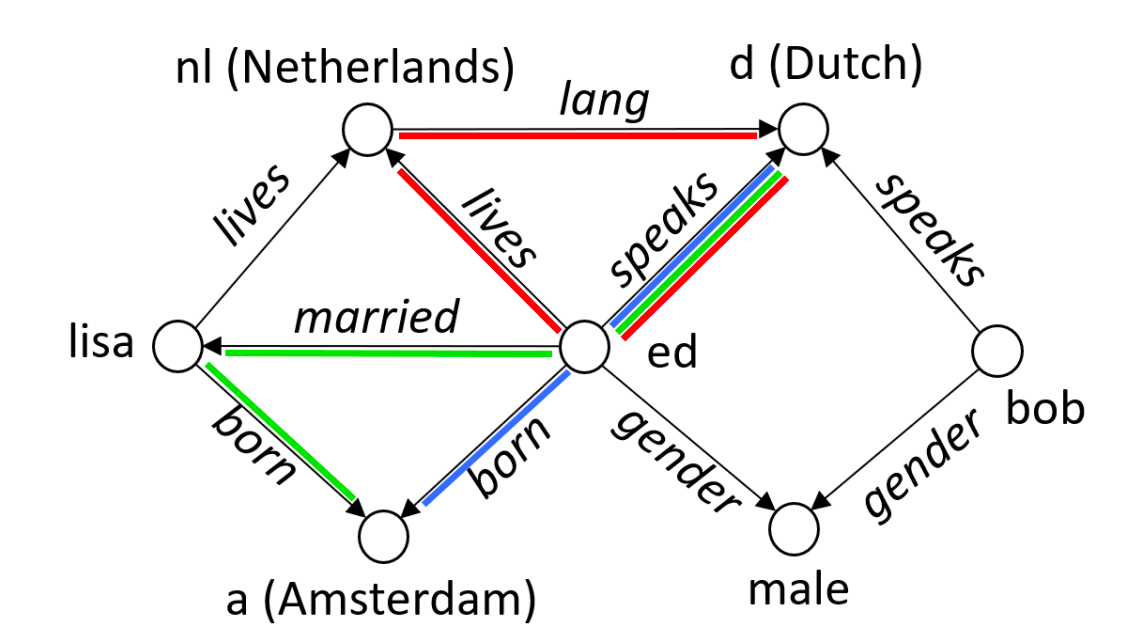
\includegraphics[width=12cm]{burl-ago.png}
	\caption{Ví dụ đồ thị tri thức}
	\label{fig:burl}
\end{figure*}

Ngoài ra Quy tắc \(B\) và quy tắc \(U_c\) cũng được gọi là quy tắc kết nối kín. Chúng có thể được học bởi hệ thống khai thác AMIE được mô tả trong \cite{AMIE,galarraga2015fast}. Quy tắc \(U_d\) là quy tắc không đóng hay đường đi không tạo thành chu trình vì \(A_n\) là biến chỉ xuất hiện một lần. Ví dụ:
\[
\begin{matrix}
	\textit{speaks}(X, Y ) & \gets & \textit{lives}(X, Y) & \quad (1) \\
	\textit{lives\_in\_city}(X, Y ) & \gets & \textit{lives}(X, A),\textit{within}(Y, A)  & \quad  (2) \\
	\textit{gen}(X, female) & \gets & \textit{married}(X, A), \textit{gen}(A, male)  & \quad  (3) \\
	\textit{profession}(X, actor) &  \gets & \textit{acted\_in}(X, A)  & \quad (4)
\end{matrix}
\]
Quy tắc (1) là quy tắc \textbf{B}(quy tắc nhị phân) quy tắc này nói rằng nếu một người (thực thể) \(X\) nói nguôn ngữ \(Y\) nếu người \(X\) sống  ở đất nước \(Y\).Rõ ràng quy tắc này là một quy tắc khái quát miễn khi nào thực thể \(X\) có cạnh nối với thực thể \(Y\) với nhãn là \textit{lives} thì có thể kết thêm 1 cạnh với nhãn \textit{speaks} giữa \(X\) và \(Y\). Quy tắc (2), (3) điều là quy tắc \(U_c\) ,quy tắc (2) nói rằng người \(X\) sống ở thành phố \(Y\) nếu người \(X\) sống ở quốc gia \(A\) và thành phố \(Y\) nằm trong quốc gia \(A\), quy tắc (3) nói rằng nếu một người \(X\) là nữ nếu họ kết hôn với một người \(A\) và người \(A\) có giới tính nam. Ở quy tắc (3) không tạo thành chu trình trên đồ thị như quy tắc (2) đỉnh (Y) lặp lại  ở \textit{head atom} và đỉnh cuối cùng trong \textit{body atoms}. Quy tắc (4) là quy tắc \(U_d\) nói rằng người \(X\) là một điễn viên nếu người \(X\) đóng trong một bộ phim \(A\).

Tất cả các quy tắc được xem xét sẽ được lọc lại đựa trên điểm được gọi là độ tin cậy của quy tắc là được đo trên tập dữ liệu huấn luyện. Độ tin cậy này được đo bằng tỷ lệ body atoms dẫn đến head atoms chia cho tất cả các đường đẫn chứa body atoms.Ví dụ khi ta có quy tắc sau:
\(\textit{gen}(X, female) \gets \textit{married}(X, A), \textit{gen}(A, male) \). Khi đó chúng ta thực hiện đếm tất cả các cặp thực thể có quan hệ  \(\textit{married}(X, A), \textit{gen}(A, male) \) được gọi là số đường dẫn chứa body atoms, sau đó thực hiện đếm tất cả các  thực thể thỏa quan hệ \(\textit{gen}(X, female) \gets \textit{married}(X, A), \textit{gen}(A, male) \) được gọi là số body atoms dẫn đến head atoms. Sau đó chia số body atoms dẫn đến head atoms cho  đường dẫn chứa body atoms được gọi là độ tin cậy của quy tắc.

\section{Thuật toán AnyBURL} \label{myalgorithm}
Trong phần này chúng tôi mô tả lại thuật toán chính của phương pháp AnyBURL nó cũng được mô tả trong \cite{burl} cũng như hai thuật toán mở rộng của chúng tôi để giải quyết vấn đề khi đồ thị được thêm một hoặc một lượng tri thức mới (thêm cạnh). Ngoài ra chúng tôi cũng mô tả sơ lược lại cách khởi tạo một luật cũng như cách thức tính toán độ tin cậy bằng cách lấy mẫu trên tập huấn luyện và vấn đề độ tin cậy khi dự đoán một luật khi tính toán độ tin cậy bằng việc lấy mẫu.
\subsection{AnyBURL}
\begin{algorithm}
	\caption{Anytime Bottom-up Rule Learning}\label{algorithm1}
	\begin{algorithmic}[1]
		\Procedure{AnyBURL($\mathbb{G}$, s, sat, Q, ts)}{}
		\State $\textit{n} = \text{2}$
		\State $R = \emptyset$
		\Loop
		\State $R_s = \emptyset$
		\State $start = currentTime()$
		\Repeat
		\State $p = samplePath(\mathbb{G}, n)$
		\State $R_p = generateRules(p)$
		\For {$r \in R_p$}
		\State $score(r, s)$
		\If {$Q(r)$}
		\State $R_s = R_s \cup \{r\}$
		\EndIf
		\EndFor
		\Until {$currentTime() > start + ts$}
		\State $R^{\prime}_s = R_s \cap R$
		\If {$ \mid R^{\prime} \mid / \mid R \mid > SAT$}
		\State $n = n + 1$
		\EndIf
		\State $R = R_s \cap R$
		\EndLoop
		\Return R
		\EndProcedure
	\end{algorithmic}
\end{algorithm}

Đầu vào của thuật toán \(\mathbb{G}, S, SAT, Q, TS\). Đầu ra là tập hợp \(R\) các luật học được. Trong đó \(\mathbb{G}\) là một đồ thị tri thức được cho từ tập dữ liệu đào tạo. \(S\) là tham số cho biết kích thước của một lần lấy mẫu trên dữ liệu đào tạo để tính toán độ tin cậy. \(SAT\) cho biết độ bão hòa(saturation) của các luật được sinh ra trong 1 lần lặp độ bão hòa này được tính bằng số luật \textbf{mới} học được ở lần lặp hiện tại so với số luật đã học được. Nếu nhỏ hơn độ bão hòa thì chúng tôi cho rằng vẫn còn tiềm năng để khai thác các luật với độ dài \(n\). Ngược lại chúng tôi tăng độ dài của luật sau đó tiếp tục khai thác. \(Q\) là một ngưỡng để xác định xem luật mới được sinh ra có được thêm vào kết quả trả về hay không. Còn \(TS\) cho biết thời gian học của thuật toán. Chúng tôi bắt đầu với \(n\) bằng \(2\) tức là các luật có độ dài đường đẫn bằng 2 vì trong path rule yêu cầu ít nhất 1 literal trong head atom và 1 trong body atoms. Ở phần lấy mẫu 1 luật(\textit{samplePath}) chỉ đơn giản là chúng ta chọn một đỉnh bất kì trong đồ thị duyệt qua tất cả các đường đẫn từ đỉnh đó đi qua \(n\) đỉnh khác, sau đó chọn ngẫu nhiên một đường đẫn trong số các trường đẫn duyệt được.

\subsection{Tạo luật}
\begin{algorithm}
	\caption{Generate Rules(p)}\label{algorithm2}
	\begin{algorithmic}[1]
		\Procedure{generate\_rules(p)}{}
		\State $\textit{generalizations} = \emptyset$
		\State $is\_binary\_rule = random.choices([true,false])$
		\If {$is\_binary\_rule$}
		\State $replace\_all\_head\_by\_variables(p)$
		\State $replace\_all\_tail\_by\_variables(p)$
		\State $add(generalizations, p)$
		\Else:
		\State $replace\_all\_head\_by\_variables(p)$
		\State $add(generalizations, p)$
		\State $replace\_all\_tail\_by\_variables(p)$
		\State $add(generalizations, p)$
		\EndIf
		\Return $generalizations$
		\EndProcedure
	\end{algorithmic}
\end{algorithm}

Ở thuật toán này chúng tôi thay các hằng số vào các head và tail trong toàn bộ path rule  của luật được lấy mẫu ở bước trước nếu luật cần học là luật nhị phân ngược lại chúng tôi chỉ thay hoặc head hoặc tail rồi thêm vào luật trả về sau đó chúng tôi lấy mẫu trên tập huấn luyện 1 tập hợp các luật sau đó tính toán độ tin cây như được mô tả trong phần \hyperref[kg]{2.3.2}. Để giảm chi phí tính toán chúng tôi chọn cách lấy mẫu trên tập huấn luyện để tính toán. Khi đưa ra dự đoán các ứng cử viên của một luật chúng tôi sẽ tính toán lại bằng cách thêm vào một lượng biểu diễn số luật bị sai mà chúng tôi chưa nhìn thấy trong quá trình lấy mẫu để tính toán độ tin cậy. Đối với mô hình của chúng thôi sau khi thử nghiệm tham số trong khoảng \([5, 10]\) cho kết quả tốt nhất.
\section{Thuật toán AnyBURL mở rộng}
\subsection{Thuật toán 3 học offline-to-online}

\begin{algorithm}
	\caption{AnyBURL Learning batch size}\label{algorithm3}
	\begin{algorithmic}[1]
		\Procedure{AnyBURLbatch($\mathbb{G}$, s, sat, Q, ts, batch\_edge)}{}
		\State $is\_connected = add(\mathbb{G}, batch\_edge)$
		\If {$is\_connected$}
		\State  $ G^{\prime} = \mathbb{G} \oplus batch\_edge$
		\Else
		\State  $ G^{\prime} = batch\_edge$
		\EndIf
		\State $\textit{n} = \text{2}$
		\State $R = \emptyset$
		\Loop
		\State $R_s = \emptyset$
		\State $start = currentTime()$
		\Repeat
		\State $p = samplePath(batch\_edge, n)$
		\State $R_p = generateRules(p)$
		\For {$r \in R_p$}
		\State $score(r, s)$
		\If {$Q(r)$}
		\State $R_s = R_s \cup \{r\}$
		\EndIf
		\EndFor
		\Until {$currentTime() > start + ts$}
		\State $R^{\prime}_s = R_s \cap R$
		\If {$ \mid R^{\prime} \mid / \mid R \mid > SAT$}
		\State $n = n + 1$
		\EndIf
		\State $R = R_s \cap R$
		\EndLoop
		\Return R
		\EndProcedure
	\end{algorithmic}
\end{algorithm}

Thuật toán này là phần bổ xung của chúng tôi để tránh việc phải đào tạo lại toàn bộ mô hình khi có một lượng tri thức mới được thêm vào đồ thị. Khi thêm vào đồ thị chúng tôi kiểm trả xem phần tri thức mới có kết nối với tri thức cũ hay không (tính liên thông) nếu có chúng tôi thực hiện phép toán \(\oplus\) lấy  tất cả các phần trong \(batch\_edge\) thêm với 1 phần liên thông với những cạnh liên thông với đồ thị với dộ dài là \(5\), Nếu không chúng tôi lấy tất cả các phần trong \(batch\_edge\) sau đó thực hiện lại các bước như thuật toán Anytime Bottom-up Rule Learning.

\subsection{Thuật toán 4 học online-to-online}
\begin{algorithm}
	\caption{AnyBURL Learning batch size}\label{euclid}
	\begin{algorithmic}[1]
		\Procedure{AnyBURLbatch($\mathbb{G}$, s, sat, Q, ts, edge)}{}
		\State $is\_connected = add(\mathbb{G}, edge)$
		\State $R = \emptyset$
		\If {$is\_connected$}
		\State $\textit{n} = \text{2}$
		\State $R_s = \emptyset$
		\Repeat
		\State $p = samplePath(edge, n)$
		\State $R_p = generateRules(p)$
		\For {$r \in R_p$}
		\State $score(r, s)$
		\If {$Q(r)$}
		\State $R_s = R_s \cup \{r\}$
		\EndIf
		\EndFor
		\Until {$currentTime() > start + ts$}
		\State $R^{\prime}_s = R_s \cap R$
		\If {$ \mid R^{\prime} \mid / \mid R \mid > SAT$}
		\State $n = n + 1$
		\EndIf
		\State $R = R_s \cap R$
		\State \Return R
		\EndIf
		\EndProcedure
	\end{algorithmic}
\end{algorithm}

Thuật toán này là một phần bổ xung cho thuật toán 3 ở trên. Sở dĩ chúng tôi gọi là online-to-online là vì khi có một cạnh mới(tri thức mới) được thêm vào đồ thị chúng tôi sẽ thực hiện việc học ngay tức khắc trên các path rule liên quan tới cạnh đó không giống như ở thuật toán 3 khi có đủ 1 lượng tri thức mới được thêm vào.


% Phương pháp dựa trên học sâu
\chapter{Phương pháp dựa trên học sâu}
\label{chap:DeeLearning}
% \section{Phương pháp dựa trên học sâu - CGAT}
% Trong phần này chúng tôi trình bày về đồ thị tri thức, và mô tả lại bài toán nhúng đồ thị (Graph Embedding), sơ lược về các kỹ thuật nhúng đồ thị hiện tại. Cùng với đó chúng ta sẽ trình bày phương pháp GAT (Graph Attention Network) và phương pháp KBAT.

Trong phần này chúng tôi trình bày về Đồ Thị Tri Thức (Knowledge Graph), và mô tả lại bài toán Nhúng Đồ Thị (Graph Embedding), sơ lược về các kỹ thuật nhúng đồ thị hiện tại. Chúng tôi sẽ trình bày lại về cơ chế chú ý cũng như cách cơ chế chú ý được áp dụng vào trong đồ thị tri thức bằng mô hình GAT\cite{velivckovic2017graph}. Đồng thời, chúng tôi sẽ trình bày một phương pháp cải tiến dựa trên mô hình mạng đồ thị chú ý là mô hình KBGAT\cite{nathani2019learning} bằng cách bổ sung thêm thông tin quan hệ và các quan hệ lân cận .
% Cuối cùng chúng ta đưa ra đề xuất của chúng ta dựa trên các mô hình trên bằng cách cộng tác thay vì ghép các lớp chú ý lại với nhau.

\section{Nhúng đồ thị}
\label{sec:graphEmbedding}

Trong thế giới thực, việc biểu diễn các thực thể và quan hệ thành các vector có thể được hiểu một cách tường minh là quá trình ánh xạ các đặc trưng, các đặc tính của một đối tượng nào đó xuống không gian có số chiều thấp hơn với mỗi thành phần đại diện cho một đặc trưng đơn vị nào đó.
Ví dụ, ta biết Donald Trump cao 1m9 và có người vợ là Melania, vì vậy ta có thể biểu diễn thực thể Donald Trump thành một vector

$\overrightarrow{e_\text{Trump}} = [1.9_{\text{heigh}}, 0_{\text{area}}, 1_\text{wife is Melania}, 0_\text{wife is Taylor}]$. Với các đặc trưng không thể đo hoặc không có giá trị ($._{\text{area}}$) sẽ bằng 0, với các đặc trưng là giá trị mà không có độ lớn ($._{\text{wife}}$) thì ta chia thành độ lớn là xác suất của các đặc trưng thành phần đơn vị ($._{\text{wife is Melania}}$, $._{\text{wife is Taylor}}$). Như vậy mọi đối tượng trong thế giới thực đều các có thể \textit{nhúng} thành các vector một cách tường minh.

Để tìm hiểu về các phương pháp và kỹ thuật \textit{nhúng đồ thị} (graph embedding) cần hiểu các định nghĩa cơ bản như sau :

\begin{itemize}
	\item
	\begin{definition}[Lân Cận Bậc Nhất]\label{def:firstOrderProximity}
		(First-Order Proximity)	giữa đỉnh $v_i$ và đỉnh $v_j$ là trọng số $A_{i, j}$ của cạnh $e_{ij}$.
	\end{definition}
	
	Hai đỉnh giống nhau hơn nếu chúng được kết nối bởi một cạnh có trọng số lớn hơn. Suy ra lân cận bậc nhất giữa đỉnh $v_i$ và $v_j$ là $s^{(1)}_{ij}$, chúng ta có $s^{(1)}_{ij} = A_{i, j}$. Gọi $s^{(1)}_{i} = \begin{bmatrix} s^{(1)}_{i1}, s^{(1)}_{i2}, \dots, s^{(1)}_{i \mid V \mid} \end{bmatrix}$ biểu thị lân cận bậc nhất giữa \(v_i\) và các đỉnh khác. Lấy biểu đồ trong hình \ref{fig:graphInput} làm ví dụ, lân cận bậc nhất $v_1$ và $v_2$ là trọng số của cạnh $e_{12}$, ký hiệu là $s^{(1)}_{12} = 1.2$. Và $s^{(1)}_1$ ghi lại trọng số của các cạnh kết nối $v_1$ và các đỉnh khác trong đồ thị, tức là, $s^{(1)}_{1} = \begin{bmatrix}  0, 1.2, 1.5, 0, 0, 0, 0, 0, 0 \end{bmatrix} $.
	
	\item
	\begin{definition}[Lân Cận Bậc Hai]\label{def:secondOrderProximity} (Second-Order Proximity)
		$s^{(2)}_{ij}$ ở giữa đỉnh $v_i$ và $v_j$ là sự tương đồng giữa $v^{\prime}_i$ vùng lân cận $s^{(1)}_i$ và $v^{\prime}_j$ vùng lân cận $s^{(1)}_j$
	\end{definition}
	
	Lấy hình \ref{fig:graphInput} làm ví dụ: $s^{(2)}_{12}$ là điểm tương đồng giữa $s^{(1)}_{1}$ và $s^{(1)}_{2}$. Như đã giới thiệu trước, $s^{(1)}_1 = \begin{bmatrix} 0, 1.2, 1.5, 0, 0, 0, 0, 0, 0 \end{bmatrix}$ và $s^{(1)}_2 = \begin{bmatrix} 1.2, 0, 0.8, 0, 0, 0, 0 , 0, 0 \end{bmatrix}$. Chúng ta hãy xem xét các điểm tương đồng cosine $s^{(2)}_{12} = cosine (s^{(1)}_1, s^{(1)}_2) = 0.43$ và $s^{(2)}_{15} = cosine(s^{(1)}_1, s^{(1)}_5) = 0$. Chúng ta có thể thấy rằng lân cận bậc hai giữa $v_1$ và $v_5$ bằng $0$ vì $v_1$ và $v_5$ không chia sẻ bất kỳ hàng xóm $1$ hop phổ biến nào. $v_1$ và $v_2$ chia sẻ một hàng xóm chung $v_3$, do đó khoảng cách thứ hai $s^{(2)}_{12}$ của chúng lớn hơn 0.
	
	Các độ đo lân cận bậc cao hơn (higher-order proximity) có thể được định nghĩa tương tự. Ví dụ, lân cận cách thứ $k-th$ giữa đỉnh $v_i$ và $v_j$ là sự tương đồng giữa $s^{(k 1)}_i$ và $s^{(k 1)}_j$.
	
	\item
	\begin{definition}[Nhúng đồ thị]\label{def:graphEmbedding}
		Cho đầu vào của đồ thị \(\mathcal{G} = (V, E)\) và số chiều được xác định trước của nhúng $d (d \ll \mid V \mid)$, vấn đề nhúng đồ thị là chuyển $\mathcal{G}$ thành một không gian \(d\)-chiều, trong đó thuộc tính đồ thị được lưu giữ càng nhiều càng tốt. Thuộc tính đồ thị có thể được định lượng bằng cách sử dụng các biện pháp lân cận như lân cận bậc nhất và bậc cao hơn. Mỗi đồ thị được biểu diễn dưới dạng một vector $d$ chiều (cho toàn bộ đồ thị) hoặc một tập các vector $d$ chiều với mỗi vector biểu thị việc nhúng một phần của đồ thị (ví dụ: đỉnh, cạnh, cấu trúc con).
	\end{definition}
\end{itemize}

Nhúng đồ thị là quá trình biến đổi các đặc trưng của đồ thị thành các vector hoặc tập hợp những vector có số chiều thấp. Càng nhúng hiệu quả, thì kết quả của độ chính xác trong việc khai thác và phân tích đồ thị sau đó càng cao. Thách thức lớn nhất của việc nhúng đồ thị phụ thuộc vào cách thiết lập của bài toán (problem setting), bao gồm đầu vào nhúng và đầu ra nhúng như trình bày ở hình \ref{fig:graphEmbeddingSettingTree}.

\begin{figure}[htp]
	\centering
	\resizebox{0.8\textwidth}{!}{%
		\begin{tikzpicture}[
			rec/.style  = {draw, text width=2cm, font=\sffamily, rectangle, thin},
			root/.style = {rec, rounded corners=6pt, align=center, fill=green!60, text width=10em},
			level 1/.style={sibling distance=8cm},
			level 2/.style={rec, rounded corners=6pt, fill=green!30,align=center, text width=10em},
			level 3/.style = {rec, align=left, fill=pink!30, text width=9.5em, yshift=-20pt},
			edge from parent/.style={->,draw, very thick},
			>=latex]
			
			% root of the the initial tree, level 1
			\node[root] {Nhúng đồ thị}
			child {node[level 2] (c1) {Đầu vào nhúng đồ thị}}
			child {node[level 2] (c2) {Đầu ra nhúng đồ thị}};
			
			% The second level, relatively positioned nodes
			\begin{scope}[every node/.style={level 3}]
				\node [below of = c1, xshift=30pt, yshift=15pt, xshift=15pt] (c11) {Đồ thị đồng nhất};
				\node [below of = c11, yshift=5pt] (c12) {Đồ thị không đồng nhất};
				\node [below of = c12, yshift=-5pt] (c13) {Đồ thị với thông tin phụ trợ};
				\node [below of = c13, yshift=-13pt] (c14) {Đồ thị cấu trúc từ dữ liệu phi quan hệ};
				
				\node [below of = c2, xshift=30pt, yshift=15pt, xshift=15pt] (c21) {Nhúng đỉnh};
				\node [below of = c21, yshift=15pt] (c22) {Nhúng cạnh};
				\node [below of = c22, yshift=15pt] (c23) {Nhúng kết hợp};
				\node [below of = c23, yshift=5pt] (c24) {Nhúng toàn bộ đồ thị};
			\end{scope}
			
			% lines from each level 1 node to every one of its "children"
			\foreach \value in {1,...,4}
			\draw[->] (c1.195) |- (c1\value.west);
			
			\foreach \value in {1,...,4}
			\draw[->] (c2.195) |- (c2\value.west);
		\end{tikzpicture}
	}
	\caption{Các kỹ thuật nhúng đồ thị}
	\label{fig:graphEmbeddingSettingTree}
\end{figure}

Dựa trên đầu vào nhúng ta phân loại thành các nhóm phương pháp đã khảo sát ở \cite{cai2018comprehensive} như sau : 
Đồ thị đồng nhất (homogeneous graph)
Đồ thị không đồng nhất (heterogeneous graph)
Đồ thị với thông tin phụ trợ (graph with auxiliary information)
Độ thị cấu trúc từ dữ liệu phi-quan hệ (graph constructed from non-relational data).

Các loại đầu vào nhúng khác nhau mang thông tin khác nhau được giữ lại trong không gian nhúng và do đó đặt ra những thách thức khác nhau đối với vấn đề nhúng đồ thị. 
Ví dụ, khi nhúng một đồ thị chỉ với thông tin cấu trúc, các kết nối giữa các đỉnh là mục tiêu cần được lưu giữ. Tuy nhiên, đối với đồ thị có nhãn đỉnh hoặc thông tin thuộc tính của một thực thể, thông tin phụ trợ cung cấp thuộc tính đồ thị từ các ngữ cảnh khác và do đó cũng có thể được xem xét trong quá trình nhúng. Không giống như đầu vào nhúng (embedding input) được cho từ các tập dữ liệu và cố định, đầu ra nhúng (embedding output) được xác định theo từng nhiệm vụ cụ thể.
Ví dụ, loại đầu ra nhúng phổ biến nhất là nhúng đỉnh, đại diện cho các đỉnh đóng vai trò như các vector thể hiện độ tương tự giữa các đỉnh. Việc nhúng đỉnh có thể có lợi cho các bài toán liên quan đến đỉnh như phân loại đỉnh, phân cụm đỉnh, v.v.

Tuy nhiên, trong một số trường hợp, các bài toán có thể liên quan đến độ chi tiết cao hơn của đồ thị, ví dụ: cặp đỉnh, đồ thị con, toàn bộ đồ thị. Do đó, thách thức đầu tiên về nhúng là tìm ra loại đầu ra nhúng phù hợp cho ứng dụng quan tâm. Có 4 loại đầu ra nhúng được minh họa ở hình \ref{fig:graphInput} gồm : Nhúng Đỉnh (Node Embedding \ref{fig:nodeEmbedding}), Nhúng Cạnh (Edge Embedding \ref{fig:edgeEmbedding}), Nhúng Kết Hợp (Hybrid Embedding \ref{fig:substructureEmbedding}) và Nhúng Toàn Bộ Đồ Thị (Whole-Graph Embedding \ref{fig:wholeGraphEmbedding}). Các mức độ chi tiết đầu ra khác nhau có các tiêu chí khác nhau sẽ có thách thức khác nhau. Ví dụ, một đỉnh nhúng tốt lưu giữ sự tương tự với các đỉnh lân cận của nó trong không gian nhúng. Ngược lại, việc nhúng toàn bộ đồ thị tốt thể hiện toàn bộ đồ thị dưới dạng một vector sao cho độ tương tự ở mức đồ thị được giữ nguyên.

\subsection{Phương pháp thiết lập bài toán nhúng đồ thị}

Với các đầu vào đã được thiết lập phụ thuộc vào thông tin cần lưu giữ, trong khi đó đầu ra thay đổi tùy theo mục tiêu khai thác đồ thị mà chúng ta mong muốn. Vì vậy ở đây chúng tôi đề cập chi tiết hơn đến các phương pháp thiết lập đồ thị theo kết quả đầu ra trong bài toán nhúng đồ thị.

\textbf{Nhúng đỉnh}
\label{sec:nodeEmbedding}

\begin{figure}[htp]
	\centering
	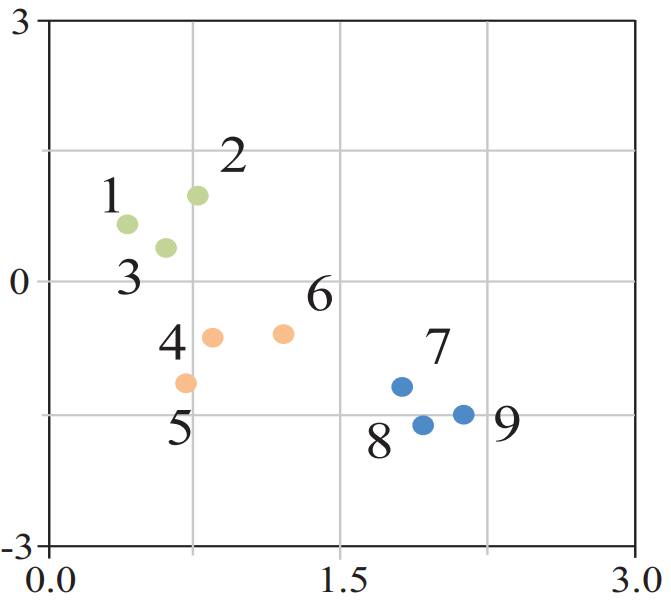
\includegraphics[width=7 cm]{images/graph_emb_2.png}
	\caption{
		Nhúng đỉnh với từng vector thể hiện đặc trưng của từng đỉnh}
	\label{fig:nodeEmbedding}
\end{figure}

Nhúng đỉnh (node embedding) biểu diễn mỗi đỉnh như một vector trong không gian số chiều thấp. Các đỉnh \textit{gần} trong đồ thị được nhúng có các biểu diễn vector tương tự nhau. Sự khác biệt giữa các phương pháp nhúng đồ thị khác nhau nằm ở cách chúng xác định \textit{độ gần nhau} giữa hai đỉnh. Lân cận bậc nhất (Định nghĩa \ref{def:firstOrderProximity}) và lân cận bậc hai (Định nghĩa \ref{def:secondOrderProximity})) là hai số liệu thường được sử dụng để tính độ tương tự đỉnh theo cặp. Trong một nghiên cứu, sự gần nhau bậc cao cũng được khám phá ở một mức độ nhất định. Ví dụ nắm bắt các quan hệ hàng xóm k-step (k = 1, 2, 3, ···) trong quá trình nhúng của chúng được đề cập trong nghiên cứu của nhóm tác giả Cao, Shaosheng\cite{cao2015grarep}.

\textbf{Nhúng cạnh}
\label{sec:edgeEmbedding}

\begin{figure}[htp]
	\centering
	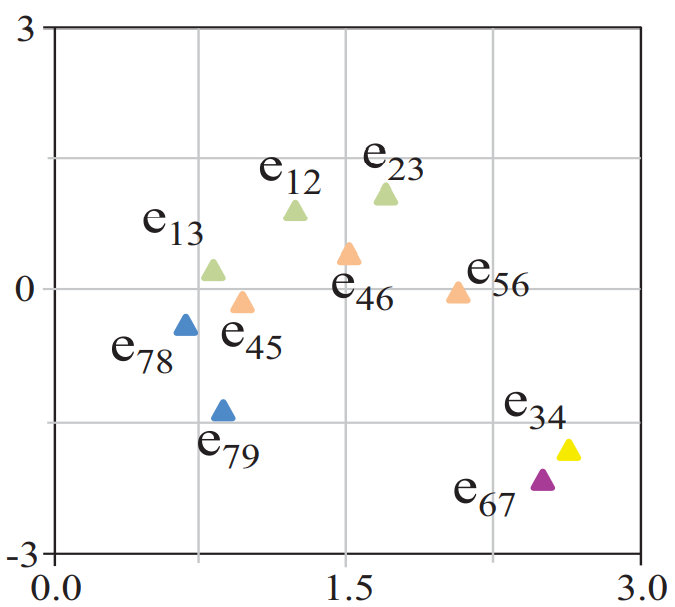
\includegraphics[width=7 cm]{images/graph_emb_3.png}
	\caption{Nhúng cạnh với từng vector thể hiện đặc trưng của từng cạnh}
	\label{fig:edgeEmbedding}
\end{figure}

Trái ngược với nhúng đỉnh, nhúng cạnh (edge embedding) nhằm mục đích biểu diễn một cạnh dưới dạng vector có số chiều thấp. Nhúng cạnh hữu ích trong hai trường hợp sau :

Thứ nhất, nhúng đồ thị tri thức. Mỗi cạnh là một bộ ba $\langle h, r, t \rangle$ (Định nghĩa \ref{def:knowledgeGraph}). Phép nhúng được học để bảo toàn r giữa h và t trong không gian nhúng, để một thực thể hoặc quan hệ bị thiếu có thể được dự đoán chính xác với hai thành phần còn lại trong $\langle h, r, t \rangle$.

Thứ hai, một số công việc nhúng một cặp đỉnh làm đặc trưng vector để làm cho cặp đỉnh này có thể so sánh với các đỉnh khác hoặc dự đoán sự tồn tại của một liên kết giữa hai đỉnh. Việc nhúng cạnh mang lại lợi ích cho việc phân tích đồ thị liên quan đến cạnh (cặp đỉnh), chẳng hạn như dự đoán liên kết, thực thể biểu diễn tri thức/dự đoán quan hệ, v.v.

\textbf{Nhúng Kết Hợp}

\begin{figure}[htp]
	\centering
	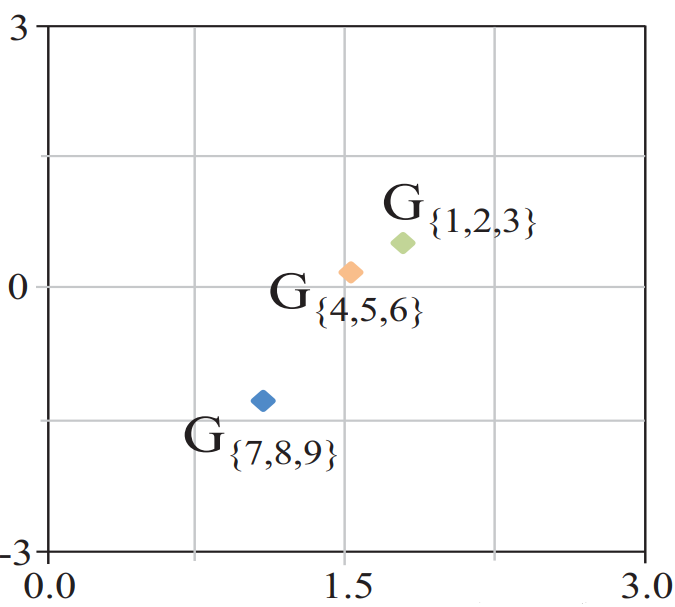
\includegraphics[width=6 cm]{images/graph_emb_4.png}
	\caption{Nhúng một cấu trúc bộ phận của đồ thị}
	\label{fig:substructureEmbedding}
\end{figure}

Nhúng kết hợp (hybrid embedding) là nhúng kết hợp các loại thành phần đồ thị khác nhau, ví dụ: đỉnh + cạnh (tức là cấu trúc con), đỉnh + bộ phận. Việc nhúng cấu trúc con hoặc bộ phận cũng có thể được bắt nguồn bằng cách tổng hợp các đỉnh riêng lẻ và nhúng cạnh bên trong nó. Tuy nhiên, kiểu tiếp cận \textit{gián tiếp} như vậy không được tối ưu hóa để thể hiện cấu trúc của đồ thị. Hơn nữa, nhúng đỉnh và nhúng bộ phận có thể củng cố lẫn nhau. Nhúng đỉnh tốt hơn vì nó học được cách phối hợp từ sự quan tâm của nhóm lân cận bậc cao, nhúng bộ phận tốt hơn khi phát hiện chính xác hơn đỉnh nhúng được tạo ra.

\textbf{Nhúng Toàn Bộ Đồ Thị}

\begin{figure}[htp]
	\centering
	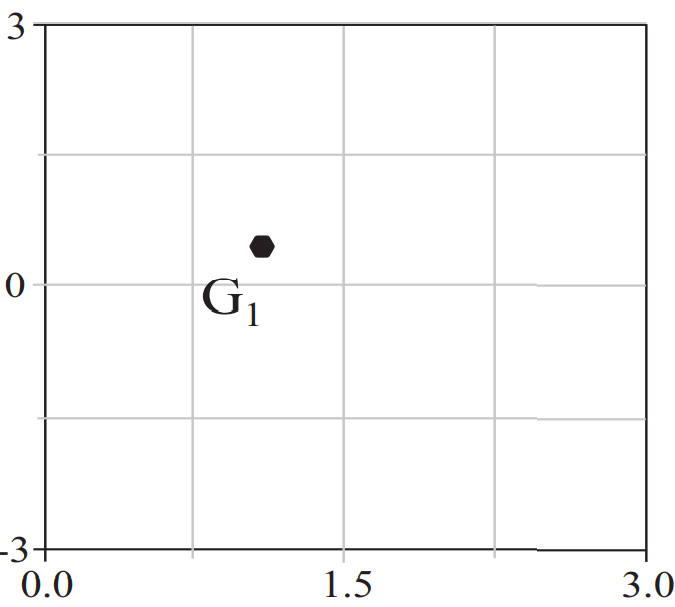
\includegraphics[width=6 cm]{images/graph_emb_5.png}
	\caption{Nhúng toàn bộ đồ thị}
	\label{fig:wholeGraphEmbedding}
\end{figure}

Nhúng toàn bộ đồ thị (whole-graph embedding) thường dành cho các đồ thị nhỏ, chẳng hạn như protein, phân tử, v.v. Trong trường hợp này, một đồ thị được biểu diễn dưới dạng một vector và hai đồ thị tương tự được nhúng để gần nhau hơn. Việc nhúng toàn bộ đồ thị mang lại lợi ích cho nhiệm vụ phân loại đồ thị bằng cách cung cấp một giải pháp đơn giản và hiệu quả để tính toán độ tương đồng của đồ thị. Để thiết lập sự thỏa hiệp giữa thời gian nhúng (tính hiệu quả) và khả năng lưu giữ thông tin (tính biểu đạt), phương pháp Nhúng đồ thị phân cấp \cite{mousavi2017hierarchical} thiết kế một khung nhúng đồ thị phân cấp. Nó cho rằng sự hiểu biết chính xác về thông tin đồ thị toàn cục đòi hỏi phải xử lý các cấu trúc con ở các quy mô khác nhau. Một kim tự tháp đồ thị được hình thành trong đó mỗi cấp là một đồ thị tóm tắt ở các tỷ lệ khác nhau. Biểu đồ được nhúng ở tất cả các cấp và sau đó được nối thành một vector. Việc nhúng toàn bộ đồ thị yêu cầu thu thập được thông tin thuộc tính của toàn bộ đồ thị, và vì vậy sẽ tốn nhiều thời gian hơn các phương pháp thiết lập khác.

\subsection{Các kỹ thuật nhúng đồ thị}

\begin{figure}[htp]
	\centering
	\resizebox{\textwidth}{!}{
		\begin{tikzpicture}[
			rec/.style  = {draw, text width=2cm, font=\sffamily, rectangle, thin},
			root/.style = {rec, rounded corners=6pt, align=center, fill=green!60, text width=10em},
			level 1/.style={sibling distance=50mm},
			level 2/.style={rec, rounded corners=6pt, fill=green!30,align=center, text width=8em},
			level 3/.style = {rec, align=left, fill=pink!30, text width=8em, yshift=-20pt},
			edge from parent/.style={->,draw, very thick},
			>=latex]
			
			% root of the the initial tree, level 1
			\node[root] {Kỹ thuật nhúng đồ thị}
			% The first level, as children of the initial tree
			child {node[level 2] (c1) {Học sâu}}
			child {node[level 2] (c2) {Phân rã ma trận}}
			child {node[level 2] (c3) {Tái cấu trúc cạnh}}
			child {node[level 2] (c4) {Đồ thị lõi}}
			child {node[level 2] (c5) {Mô hình sinh}};
			
			% The second level, relatively positioned nodes
			\begin{scope}[every node/.style={level 3}]
				\node [below of = c1, xshift=30pt] (c11) {Sử dụng bước ngẫu nhiên};
				\node [below of = c11] (c12) {Không sử dụng bước ngẫu nhiên};
				
				\node [below of = c2, xshift=30pt] (c21) {Đồ thị toán tử Laplace Eigenmaps};
				\node [below of = c21] (c22) {Phân rã ma trận bằng xấp xỉ đỉnh};
				
				\node [below of = c3, xshift=25pt] (c31) {Cực đại hóa xác suất tái cấu trúc cạnh};
				\node [below of = c31, yshift=-20pt] (c32) {Tối thiểu hóa mất mát dựa trên khoảng cách};
				\node [below of = c32, yshift=-20pt] (c33) {Tối thiểu hóa xếp hạng mất mát dựa trên lề};
				
				\node [below of = c4, xshift=25pt] (c41) {Dựa trên graphlet};
				\node [below of = c41] (c42) {Dựa trên mẫu nhánh cây};
				\node [below of = c42] (c43) {Dựa trên bước nhảy ngẫu nhiên};
				
				\node [below of = c5, xshift=30pt] (c51) {Nhúng đồ thị dựa trên không gian ẩn};
				\node [below of = c51] (c52) {Nhúng kết hợp ngữ nghĩa};
			\end{scope}
			
			% lines from each level 1 node to every one of its "children"
			\foreach \value in {1,2}
			\draw[->, very thick] (c1.195) |- (c1\value.west);
			
			\foreach \value in {1, 2}
			\draw[->, very thick] (c2.195) |- (c2\value.west);
			
			\foreach \value in {1,...,3}
			\draw[->, very thick] (c3.195) |- (c3\value.west);
			
			\foreach \value in {1,...,3}
			\draw[->, very thick] (c4.195) |- (c4\value.west);
			
			\foreach \value in {1,...,2}
			\draw[->, very thick] (c5.195) |- (c5\value.west);
		\end{tikzpicture}
	}
	\caption{Các kỹ thuật nhúng đồ thị}
	\label{fig:graphEmbeddingTechniquesTree}
\end{figure}

Trong phần này, chúng tôi phân loại các nhóm phương pháp nhúng đồ thị dựa vào kỹ thuật sử dụng, như đã nói ở trên, mục tiêu của việc nhúng đồ thị là biểu diễn một đồ thị vào không gian có số chiều thấp mà vẫn giữ vững được những thông tin vốn có của đồ thị nhiều nhất có thể. Các kỹ thuật nhúng đồ thị cơ bản khác nhau ở cách định nghĩa các đặc tính vốn có của đồ thị cần được lưu giữ. Vì mục tiêu chính của chúng tôi là tìm hiểu về các nhóm phương pháp nhúng đồ thị dựa trên kỹ thuật học sâu nên chúng tôi chỉ trình bày sơ lược đối với các nhóm phương pháp khác.

\textbf{Học sâu}

Ở phần này chúng tôi sẽ trình bày chi tiết về các hướng nghiên cứu của kỹ thuật học sâu (deep learning) bao gồm : sử dụng bước nhảy ngẫu nhiên (random walk) và không sử dụng bước nhảy ngẫu nhiên. Kỹ thuật học sâu được sử dụng phổ biến trong việc nhúng đồ thị bởi vì sự nhanh chóng và hiệu quả trong việc thu thập các đặc trưng một cách tự động. Trong các phương pháp sử dụng kỹ thuật học sâu này, cả 3 loại phương pháp thiết lập đồ thị dựa trên đầu vào (ngoại trừ đồ thị cấu trúc từ dữ liệu phi-quan hệ) và 4 loại đầu ra (Hình \ref{fig:graphEmbeddingSettingTree}) đều có thể áp dụng kỹ thuật học sâu. 

\textit{Kỹ thuật học sâu với bước nhảy ngẫu nhiên}

Trong nhóm phương pháp này, lân cận bậc hai (Định nghĩa \ref{def:secondOrderProximity}) trong đồ thị sẽ được bảo đảm trong không gian nhúng bằng cách cực đại hóa xác suất của những hàng xóm quan sát của một đỉnh điều kiện trên vector nhúng của nó. Đồ thị sẽ được biểu diễn như là một tập hợp mẫu bằng cách lấy mẫu từ những bước đi ngẫu nhiên, và sau đó các phương pháp học sâu sẽ được áp dụng vào đồ thị nhúng để vẫn đảm bảo đặc tính của đồ thị mang theo thông tin đường đi. Các phương pháp sử dụng nhóm phương pháp này như : Deep Walk \cite{perozzi2014deepwalk}, LINE \cite{tang2015line}, Node2Vec \cite{grover2016node2vec}, Anonymous Walk \cite{ivanov2018anonymous}, NetGAN \cite{bojchevski2018netgan}, ...

\textit{Kỹ thuật học sâu không sử dụng bước nhảy ngẫu nhiên}

Trong phương pháp này, những cấu trúc học đa lớp sẽ được áp dụng một cách nhanh chóng và hiệu quả để biến đổi đồ thị thành không gian số chiều thấp hơn. Phương pháp này sẽ áp dụng cho toàn bộ đồ thị, có một số phương pháp phổ biến hiện nay đã được khảo sát và trình bày ở báo cáo \cite{rossi2020knowledge} như sau :

\begin{itemize}
	\item Mạng Neural Tích Chập (Convolutional Neural Networks)
	
	Mô hình này sử dụng nhiều lớp tích chập : Với mỗi lớp thực hiện tính tích chập trên dữ liệu đầu vào một bộ lọc có số chiều thấp. Kết quả là một ánh xạ đặc trưng, sau đó lại tiếp tục đi qua một lớp kết nối đầy đủ để tính giá trị xác suất. Ví dụ như \textbf{ConvE} \cite{dettmers2017convolutional} : Mỗi thực thể và mối quan hệ sẽ được biểu diễn bằng một vector số chiều thấp $d-\text{chiều}$. Với mỗi bộ ba, nó ghép và thay đổi kích thước của vector nhúng đỉnh $h$ và quan hệ $r$ vào một đầu vào duy nhất $[h, r]$ với kích thước kết quả là $d_m \times d_n$. Sau đó nó đi qua lớp tích chập với bộ lọc $\omega$ có kích thước $m \times n$, rồi đi qua một lớp kết nối đầy đủ  (fully connected layers) và các trọng số $W$. Kết quả cuối cùng được kết hợp với vector nhúng đuôi $t$ bằng cách sử dụng tích vô hướng (dot products). Kiến trúc này có thể coi là một kiến trúc \textit{phân loại các lớp} .
	
	Một mô hình phổ biến khác là \textbf{ConvKB} \cite{nguyen2017novel}, tương tự như ConvE, nhưng nó ghép cả ba vector nhúng $h$, $r$ và $t$ vào một ma trận $[h, r, t]$ kích thước $d \times 3$ chiều. Sau đó nó đi qua một lớp tích chập với $T$ bộ lọc $\omega$ kích thước $1 \times 3$. Kết quả là $T \times 3$ ánh xạ đặc trưng. Sau đó ánh xạ đặc trưng lại đi qua lớp kết nối đầy đủ và trọng số $\mathbf{W}$. Kiến trúc này có thể coi là kiến trúc phân loại nhị phân.
	
	\item Mạng Hồi Quy Tuyến Tính (Recurrent Neural Networks)
	
	Những mô hình này sẽ cho một lớp hoặc nhiều lớp hồi tuyến tính để phân tích toàn bộ đường đi (một chuỗi sự kiện/bộ ba) lấy ra từ tập huấn luyện, thay vì chỉ xử lý các sự kiện một cách riêng biệt. Ví dụ như RSN \cite{guo2019learning}, nhận thấy mô hình hồi quy tuyến tính truyền thống không phù hợp cho đồ thị, với mỗi lần thực hiện nó chỉ lấy thông tin của mối quan hệ mà không lấy thông tin của vector đỉnh của lần thực hiện trước đó. Vì vậy nó không xử lý rõ ràng sự luân chuyển các đường dẫn của các thực thể và quan hệ. Để giải quyết vấn đề này, họ đề xuất RSN (Recurrent Skipping Networks \cite{guo2019learning}) : với mỗi bước nhảy, nếu đầu vào là quan hệ, một trạng thái ẩn được cập nhật để tái sử dụng thêm vector đỉnh. Sau đó, kết quả đầu ra được nhân tích vô hướng với mỗi vector nhúng mục tiêu.
	
	\item Mạng Neural Bao Bọc (Capsule Neural Networks)
	
	Mạng bao bọc (capsule networks) sẽ sắp một nhóm neural lại với nhau gọi là viên nang \label{capsule}, mỗi viên nang này sẽ mã hóa những đặc trưng đặc biệt của đầu vào, như là đại diện cho một nhóm hình ảnh cụ thể. Ưu điểm của mạng bao bọc đó là giúp nhận ra những đặc trưng mà không mất thông tin không gian so với việc tính tích chập thông thường. Mỗi một viên nang tìm ra những đặc trưng theo kích thước vector đầu ra. Ví dụ như : \textbf{CapsE} \cite{vu2019capsule}, mỗi thực thể và quan hệ được xem là một vector nhúng như trên, tương tự như ConvKB, nó sẽ ghép ba vector nhúng $h$, $r$ và $t$ thành một ma trận nhúng kích thước $d \times 3$. Sau đó nó đi qua lớp có E bộ lọc tích chập có kích thước $1 \times 3$. Kết quả là một ma trận kích thước $d \times E$ mà với mỗi dòng thứ $i-th$ đại diện cho những thực thể $h[i]$, $t[i]$ và quan hệ $r[i]$ riêng biệt. Ma trận này sẽ đi lớp bao bọc mà mỗi viên nang (\ref{capsule}) riêng biệt xử lý mỗi cột, vì vậy nó nhận được thông tin dựa theo một đặc trưng của bộ ba đầu vào. Và lớp thứ hai với một lớp bao bọc được sử dụng để đưa ra kết quả đầu ra.
	
	\item Mạng đồ thị chú ý (Graph Attention Networks)
	
	Nhóm phương pháp này sử dụng cơ chế chú ý (attention mechanism \cite{vaswani2017attention}) mà đã đạt được kết quả cải thiện đáng kể trong xử lý ngôn ngữ tự nhiên. Ở nhóm phương pháp này với mỗi vector nhúng, các thực thể được tổng hợp thông tin chú ý từ các thực thể kế cận, sau đó các thông tin chú ý được ghép chồng với nhau và đi qua một lớp kết nối đầy đủ và trọng số để biến đổi thành các vector nhúng cuối cùng. Ví dụ như : GAT \cite{velivckovic2017graph} với mỗi bộ ba từ tập huấn luyện được nhúng và áp dụng cơ chế chú ý đa đỉnh để cho ra một vector nhúng. Sau đó vector nhúng này tiếp tục đi qua một ma trận trọng số để biến đổi thành vector nhúng mới có số chiều lớn hơn tổng hợp thông tin từ các đỉnh kế cận từ bộ ba ban đầu. Một cải tiến khác của GAT bằng cách thêm thông tin của vector nhúng quan hệ là KBGAT \cite{nathani2019learning}. Các phương pháp này được trình bày cụ thể ở các phần tiếp theo.
	
	\item Ngoài ra còn một số phương pháp khác như sử dụng kỹ thuật tự động mã hóa (autoencoder) như Mạng Nhúng Cấu Trúc Sâu (Structural Deep Network Embedding \cite{wang2016structural}) .
\end{itemize}

\textbf{Phân rã ma trận}

Phân rã ma trận (matrix factorization) dựa trên đồ thị nhúng biểu diễn những đặc tính của đồ thị (ví dụ những cặp tương đồng hay giống nhau) dưới hình thức một ma trận và phân rã ma trận này để lấy được thông tin nhúng của đỉnh. Đầu vào của nhóm phương pháp này thường là những đặc trưng phi-quan hệ nhiều chiều và đầu ra là tập hợp các đỉnh nhúng. Có hai phương pháp nhúng đồ thị dựa trên phân rã ma trận bao gồm : Đồ Thị Toán Tử Laplace Eigenmaps (Graph Laplacian Eigenmaps) và Phân Rã Ma Trận Xấp Xỉ Đỉnh (Node Proximity Matrix Factorization)

\begin{itemize}
	\item \textit{Đồ Thị Toán Tử Laplace Eigenmaps}
	
	Nhóm phương pháp này sẽ đảm bảo đặc tính của đồ thị bằng cách phân tích những cặp tương đồng và sẽ phạt nặng những đỉnh có sự tương đồng lớn hơn mà nhúng xa nhau. 
	
	\item \textit{Phân Rã Ma Trận Xấp Xỉ Đỉnh}
	
	Nhóm phương pháp này sẽ xấp xỉ các đỉnh lân cận trong một không gian số chiều thấp sử dụng kỹ thuật phân rã ma trận. Mục tiêu là để bảo toàn những đỉnh lân cận để tối thiểu hóa hàm xấp xỉ.
\end{itemize}

\textbf{Tái cấu trúc cạnh}

Phương pháp tái cấu trúc cạnh (edge reconstruction) sẽ xây dựng các cạnh dựa trên những đỉnh nhúng sao cho giống với những đồ thị đầu vào nhất có thể. Phương pháp này tối tối đa hóa xác suất tái tạo cạnh hoặc tối thiểu hóa hàm mất mát tái tạo cạnh, ngoài ra còn chia ra hàm mất mát dựa trên khoảng cách và hàm xếp hạng mất mất mát dựa trên lề .

\begin{itemize}
	\item \textit{Cực đại hóa xác suất tái cấu trúc cạnh }
	
	Ở phương pháp Cực đại hóa xác suất tái cấu trúc cạn (maximize edge reconstruct probability), một đỉnh nhúng tốt sẽ cực đại hóa xác suất sinh của các cạnh quan sát trong một đồ thị. Nghĩa là một vector đỉnh nhúng tốt sẽ được tái xây dựng lại như là đồ thị đầu vào gốc. Chúng được phân biệt bằng cách cực đại hóa xuất xuất sinh của tất cả các cạnh quan sát sử dụng vector đỉnh nhúng .
	
	\item \textit{Tối thiểu hóa mất mát dựa trên khoảng cách}
	
	Trong phương pháp tối thiểu hóa mất mát dựa trên khoảng cách (minimize distance-based loss), các đỉnh lân cận tính toán dựa trên vector đỉnh nhúng phải càng gần nhất với những đỉnh lân cận trên các cạnh đang quan sát càng tốt.
	Cụ thể là, độ gần của đỉnh có thể được tính toán dựa trên những đỉnh nhúng hoặc được tính toán theo kinh nghiệm dựa trên các cạnh được quan sát. Sau đó sẽ được tối thiểu hóa sự khác biệt giữa hai loại lân cận để đảm bảo độ gần tương ứng.
	
	\item \textit{Tối thiểu hóa xếp hạng mất mát dựa trên lề}
	
	Trong phương pháp tối thiểu xếp hạng mất mát dựa trên lề (minimize margin-based ranking loss), các cạnh của đồ thị đầu vào thể hiện sự tương quan giữa những cặp đỉnh. Một số đỉnh trong đồ thị thì thường liên kết với những tập hợp đỉnh liên quan. Cụ thể phương pháp này sẽ giúp các đỉnh vector nhúng sẽ gần nhau nếu các đỉnh liên quan đến nhau hơn so với những đỉnh không liên quan khác.
\end{itemize}

\textbf{Đồ thị lõi}

Với đồ thị lõi (graph kernel) toàn bộ cấu trúc đồ thị có thể được biểu diễn như là một vector chứa số lượng cấu trúc con cơ bản được phân tách từ đồ thị. Kỹ thuật đồ thị lõi bao gồm các nhánh phương pháp con gồm : graphlet, mẫu đồ thị con (subtree patterns) và dựa trên bước nhảy ngẫu nhiên .

Phương pháp này được thiết kế để nhúng toàn bộ đồ thị chỉ lấy đặc trưng toàn cục của toàn bộ đồ thị. Đầu vào của phương pháp này thường là đồ thị đồng nhất. hoặc đồ thị với thông tin bổ trợ

\textbf{Mô hình sinh}

Một mô hình sinh (generative model) có thể được định nghĩa bằng cách xác định sư phân phối chung của đặc trưng đầu vào và những lớp nhãn, và được điều chỉnh dựa trên một tập những tham số. Có hai nhóm phương pháp con của mô hình sinh bao gồm : Nhúng đồ thị dựa trên không gian ẩn (embed graph into latent space) và nhúng kết hợp ngữ nghĩa (incorporate semantics for embedding).
Mô hình sinh có thể được dùng cho cả nhúng đỉnh và nhúng cạnh . Nó được xem như là đỉnh những ngữ nghĩa với đầu vào thường là các đồ thị không đồng nhất hoặc đồ thị với thông tin phụ trợ.
\begin{itemize}
	\item \textit{Nhúng đồ thị trên không gian ngữ nghĩa ẩn}
	
	Với nhóm phương này, các đỉnh được nhúng vào một không gian ngữ nghĩa ẩn nơi khoảng cách giữa đỉnh mô tả được cấu trúc của đồ thị.
	
	\item \textit{Nhúng kết hợp ngữ nghĩa}
	
	Phương pháp này thì mỗi đỉnh sẽ gần với đồ thị và có ngữ nghĩa mà nó phải được nhúng gần hơn. Những đỉnh ngữ nghĩa có thể được tìm ra từ những đỉnh mô tả thông qua một mô hình sinh.
	
\end{itemize}

\textbf{Tổng kết} : Các phương pháp nhúng đồ thị đều có ưu nhược điểm riêng được nhóm tác giả Cai, Hongyun\cite{cai2018comprehensive} tổng hợp và trình bày lại ở bảng \ref{tab:graphEmbeddingTechCompare}. Với nhóm phương pháp \textit{phân rã ma trận} dựa trên đồ thị nhúng sẽ học những đại diện dựa trên việc phân tích sự tương đồng các cặp toàn cục. Với nhóm phương pháp \textit{học sâu}, những mô hình này đạt được kết quả hứa hẹn so với những phương pháp khác và phù hợp cho việc nhúng đồ thị vì nó có khả năng học được các biểu diễn phức tạp từ các cấu trúc đồ thị phức tạp. Các phương pháp sử dụng kỹ thuật bước nhảy ngẫu nhiên trong học sâu có chi phí tính toán thấp hơn so với các phương pháp sử dụng kỹ thuật học sâu. Các phương pháp truyền thống coi đồ thị như một lưới, tuy nhiên nó không giống với bản chất của đồ thị. Với nhóm phương pháp \textit{tái cấu trúc cạnh} sẽ tối ưu hàm mục tiêu dựa trên các cạnh quan sát hoặc xếp hạng các bộ ba. Nhóm phương pháp này hiệu quả hơn nhưng vector nhúng kết quả lại không quan tâm đến cấu trúc toàn cục của đồ thị. Nhóm phương pháp \textit{đồ thị lõi} chuyển đồ thị vào một vector để dễ dàng thực hiện các nhiệm vụ phân tích đồ thị như phân loại đồ thị. Vì vậy nó chỉ hiệu quả khi liệt kê những nhánh cấu trúc đơn vị mong muốn trong một đồ thị. Với nhóm phương pháp \textit{mô hình sinh}, nó tận dụng thông tin một cách tự nhiên từ nhiều nguồn khác nhau trong một mô hình duy nhất. Việc nhúng đồ thị vào không gian ngữ nghĩa ẩn tạo ra những vector nhúng có thể được diễn giải bằng cách sử dụng ngữ nghĩa. Nhưng giả định về việc lập mô hình quan sát bằng cách sử dụng các phân bố nhất định là khó có thể biện minh. Hơn nữa, phương pháp sinh cần một lượng lớn dữ liệu huấn luyện để ước tính mô hình kết quả phù hợp với dữ liệu. Vì thế nó có thể không đạt kết quả tốt cho những đồ thị nhỏ hoặc số lượng nhỏ đồ thị.
\newcolumntype{L}{>{\arraybackslash}m{5cm}}
\begin{table}[htbp]
	\begin{center}
		\caption{Bảng so sánh ưu và nhược điểm của kỹ thuật nhúng đồ thị}
		\label{tab:graphEmbeddingTechCompare}
		\resizebox{\textwidth}{!}{
			\begin{tabular}{|p{2cm}|p{8cm}|L|p{8cm}|}
				\hline
				Phương pháp & Danh mục con & Ưu điểm & Nhược điểm \\
				\hline \hline
				Phân rã ma trận & Đồ thị toán tử Laplace Eigenmap & \multirow{3}{5cm}{Xem xét toàn cục các đỉnh lân cận}&
				\multirow{2}{8cm}{Sử dụng không gian và thời gian tính toán lớn }\\
				\cline{2-2}
				& Phân rã ma trận bằng xấp xỉ đỉnh & & \\
				\hline
				\multirow{3}{2cm}{Tái cấu trúc cạnh} & Cực đại hóa xác suất tái cấu trúc cạnh & \multirow{3}{5cm}{Huấn luyện tương đối hiệu quả} & \multirow{3}{8cm}{Tối ưu chỉ sử dụng thông tin cục bộ. Ví dụ như các cạnh (hàng xóm 1 nước) hoặc cặp đỉnh xếp hạng } \\ \cline{2-2}
				& Tối thiểu hóa mất mát dựa trên khoảng cách & & \\ \cline{2-2}
				& Tối thiểu hóa xếp hạng mất mát dựa trên lề & & \\ \hline
				\multirow{3}{2cm}{Đồ thị lõi} & Dựa trên graphlet & \multirow{3}{5cm}{Hiệu quả, chỉ tính những nhánh cấu trúc đơn vị mong muốn} & \multirow{3}{8cm}{Nhánh cấu trúc thì không độc lập. Số chiều nhúng tăng lên theo hàm mũ} \\ \cline{2-2}
				& Dựa trên mẫu nhánh cây   & & \\ \cline{2-2}
				& Dựa trên bước nhảy ngẫu nhiên & & \\ \hline
				
				Mô hình sinh & Nhúng đồ thị dựa trên không gian ẩn & Phép nhúng có thể giải thích được & Khó điều chỉnh lựa chọn phân bố \\ \cline{2-3}
				
				& Nhúng kết hợp ngữ nghĩa & Tận dụng nhiều thông tin nguồn & Yêu cầu một lượng lớn dữ liệu huấn luyện một cách tự nhiên\\
				\hline
				
				Học sâu & Sử dụng bước ngẫu nhiên & \multirow{2}{5cm}{Hiệu quả và nhanh chóng Không phải trích đặc trưng} & Chỉ xem xét đến nội dung cục bộ trong một đường đi. Khó để tìm kiếm chiến lược lấy mẫu tối ưu \\ \cline{2-2} \cline{4-4} 
				& Không sử dụng bước ngẫu nhiên &  & Chi phí tính toán cao \\ \hline
			\end{tabular}
		}
	\end{center}
\end{table}

Trong các phương pháp trên, nhóm phương pháp nhúng đồ thị bằng học sâu giúp học được các biểu diễn phức tạp và đạt được kết quả hứa hẹn nhất hiện nay. Mô hình mạng chú ý trên đồ thị dựa trên cơ chế chú ý giúp tổng hợp thông tin của một thực thể dựa vào các trọng số chú ý của các thực thể lân cận đối với thực thể gốc. Chúng tôi cho rằng đây là hướng nghiên cứu tương tự như quan hệ giữa chú ý và ghi nhớ \cite{memoryandattention:2020}, sự phân bố của chú ý sẽ quyết định trọng số hay sự quan trọng của một thực thể này đối với một thực thể khác. Cũng như vector nhúng biểu diễn cho một thực thể sẽ bị ảnh hưởng bởi sự chú ý hay sự quan trọng của các vector nhúng lân cận. Vì vậy đây là hướng nghiên cứu chúng tôi chọn trong các nhóm phương pháp trên.


\section{Cơ chế chú ý đa đỉnh}

Năm 2014, cơ chế chú ý đa đỉnh (multi-head attention) được phát minh bởi nhóm tác giả Bahdanau, Dzmitry\cite{bahdanau2014neural} nhưng mãi đến năm 2017 nó mới được phổ biến thông qua mô hình Transformer của nhóm tác giả Vaswani, Ashish\cite{vaswani2017attention}. Cơ chế chú ý là một phương pháp hiệu quả giúp thể hiện sự quan trọng của một từ với các từ khác trong một câu, nó còn được chứng minh là đại diện cho bất kỳ phép tính tích chập nào trong báo cáo của nhóm tác giả Cordonnier, Jean-Baptiste\cite{cordonnier2019relationship}. Để hiểu về cách cơ chế chú ý đa đỉnh được áp dụng vào trong đồ thị, trong phần này chúng tôi sẽ trình bày lại chi tiết về cơ chế chú ý đa đỉnh để từ đó hiểu được cách cơ chế chú ý được áp dụng vào nhiệm vụ dự đoán liên kết trong đồ thị tri thức.
%cũng như cải tiến mới nhất của cơ chế chú ý đa đỉnh của nhóm tác giả Cordonnier, Jean-Baptiste\cite{cordonnier2020multi}
%
%trong phần này chúng tôi sẽ trình bày chi tiết về cơ chế chú ý đa đỉnh cũng như cải tiến mới nhất trên cơ chế chú ý đa đỉnh \cite{cordonnier2020multi} được chúng tôi gọi là \textit{cộng tác đa đỉnh chú ý} (collaborate multi-head attention).

\subsection{Cơ Chế Chú Ý (Attention Mechanism)}
\label{sec:attentionMechanism}

Đầu vào của cơ chế chú ý là hai ma trận nhúng $\mathbf{X} = \Big\{\overrightarrow{x_1}, \overrightarrow{x_2}, ...,  \overrightarrow{x_{N_x}}\Big\}$ và $\mathbf{Y} = \Big\{\overrightarrow{y_1}, \overrightarrow{y_2}, ...,  \overrightarrow{y_{N_y}}\Big\}$, với mỗi dòng $i^{\text{th}}$ hay $j^{\text{th}}$ trong ma trận $\mathbf{X}$ hay $\mathbf{Y}$ là một vector nhúng $\overrightarrow{x_i} \in \mathbb{R}^{1 \times D_{\text{in}}}$, $\overrightarrow{y_j} \in \mathbb{R}^{1 \times D_{\text{in}}}$.
Cơ chế chú ý là quá trình biến đổi vector có $D_{\text{in}}$ chiều thành vector đầu ra có $D_{\text{attention}}$ chiều để thể hiện sự quan trọng của từng $N_x$ phần tử $x$ so với tất cả $N_y$ các phần tử $y$. Với $\mathbf{X} \in \mathbb{R}^{N_x \times D_\text{in}}$ và $\mathbf{Y} \in \mathbb{R}^{N_y \times D_\text{in}}$ là các ma trận nhúng đầu vào, và $\mathbf{H} \in \mathbb{R}^{N_x \times D_\text{attention}}$ là ma trận nhúng đầu ra của cơ chế chú ý của nhóm tác giả Vaswani, Ashish\cite{vaswani2017attention} theo công thức sau :

\begin{equation}
	\label{attention}
	\mathbf{H} = \text{Attention}(\mathbf{Q}, \mathbf{K}, \mathbf{V}) = \text{softmax}\Big(\frac{\mathbf{Q}\mathbf{K}^T}{\sqrt{d_k}}\Big) \mathbf{V}
\end{equation}

với  $\mathbf{Q} = \mathbf{X}\mathbf{W}_Q, \mathbf{K} = \mathbf{Y} \mathbf{W}_K, \mathbf{V} = \mathbf{Y} \mathbf{W}_V$

Các ma trận trọng số 
$\mathbf{W}_Q \in \mathbb{R}^{D_{\text{in}} \times D_{k}}$, 
$\mathbf{W}_K \in \mathbb{R}^{D_{\text{in}} \times D_{k}}$ và 
$\mathbf{W}_V \in \mathbb{R}^{D_{\text{in}} \times D_{\text{attention}}}$ là các ma trận thể hiện quá trình tham số hóa để biến đổi các vector nhúng đầu vào $D_{\text{in}}$ chiều thành vector nhúng đầu ra có $D_{k}$ hoặc $D_{\text{attention}}$ chiều. $\mathbf{Q}\mathbf{K}^T$ là quá trình nhân tích vô hướng của từng vector nhúng $x$ ban đầu với tất cả vector nhúng y. Việc chia cho $\sqrt{d_k}$ là để chuẩn hóa theo số chiều $k$. Sau đó kết quả được chuẩn hóa lại bằng hàm \textit{softmax} để có thể so sánh giữa các hệ số chú ý khác nhau. Ta có thể coi $\text{softmax}\Big(\frac{\mathbf{Q}\mathbf{K}^T}{\sqrt{d_k}}\Big)$ là một \textit{hệ số chú ý} thể hiện sự quan trọng của từng phần từ y đối với mỗi phần tử x. Cuối cùng, kết quả được nhân với vector nhúng $\mathbf{V}$ để biến đổi từ vector nhúng $D_{k}$ chiều thành vector nhúng mới  $D_{\text{attention}}$ chiều .

Nếu $\mathbf{X} = \mathbf{Y}$ nghĩa là chúng ta đang tính sự quan trọng của một phần tử so với chính các phần tử khác trong ma trận nhúng ban đầu và ta gọi nó là cơ chế tự-chú ý (self-attention mechanism) .

\subsection{Chú Ý Đa Đỉnh (Multi-Head Attention)}

Cơ chế chú ý đa đỉnh là cách ghép các lớp chú ý ở trên lại để giúp ổn định quá trình học.
Tương tự như cơ chế chú ý ở trên, cơ chế chú ý đa đỉnh (multi-head attention mechanism) là quá trình biến đổi $N_x$ vector nhúng ban đầu $D_{\text{in}}$ chiều thành vector nhúng $D_{\text{multi-head}}$ chiều với thông tin được tổng hợp từ nhiều đỉnh khác nhau giúp ổn định trong quá trình huấn luyện. Cơ chế chú ý đa đỉnh sẽ ghép $N_{\text{head}}$ các đầu ma trận chú ý $\mathbf{H}$ rồi sau đó tiếp tục nhân với một ma trận trọng số để biến đổi từ ma trận nhúng $\mathbf{X} \in \mathbb{R}^{N_x \times D_\text{in}}$ ban đầu thành ma trận nhúng mới $\mathbf{X}' \in \mathbb{R}^{N_x \times D_{\text{multi-head}}}$ như công thức sau :

\begin{equation}
	\label{headAttention}
	\begin{split}
		\mathbf{X}'& =\left(\bigparallel_{h=1}^{N_{\text{head}}}\mathbf{H}^{(h)}\right)\mathbf{W}^{O} \\
		& = \left(\bigparallel_{h=1}^{N_{\text{head}}} \text{Attention}(\mathbf{X} \mathbf{W}_Q^{(h)}, \mathbf{Y} \mathbf{W}_K^{(h)}, \mathbf{Y} \mathbf{W}_V^{(h)}) \right)\mathbf{W}^{O}
	\end{split}
\end{equation}

Trong đó các ma trận trọng số $\mathbf{W}_Q^{(h)}$, $\mathbf{W}_K^{(h)} \in \mathbb{R}^{D_{\text{in}} \times D_{k}}$ và $\mathbf{W}_V^{(h)} \in \mathbb{R}^{D_{\text{in}} \times D_{\text{attention}}}$ thuộc vào từng lớp chú ý $h \in [N_{\text{head}}]$ khác nhau. $\mathbf{W}^{O} \in \mathbb{R}^{N_{\text{head}} D_{\text{attention}} \times D_{\text{multi-head}}}$ để tham số hóa quá trình biến đổi ma trận các đỉnh đã ghép thành một ma trận nhúng kết quả cuối cùng.

Đến đây chúng tôi đã trình bày về cơ chế chú ý tính hệ số chú ý và tổng hợp thông tin nhúng từ các vector nhúng lân cận. Trong phần tiếp theo chúng tôi sẽ trình bày về cách cơ chế chú ý được áp dụng vào trong đồ thị tri thức .

%\textbf{Lớp cộng tác đa đỉnh chú ý}

%\cite{weng2018attention}

\section{Mạng đồ thị chú ý}
\label{sec:GAT}

\begin{figure}[htp]
	\centering
	\resizebox{\textwidth}{!}{%
		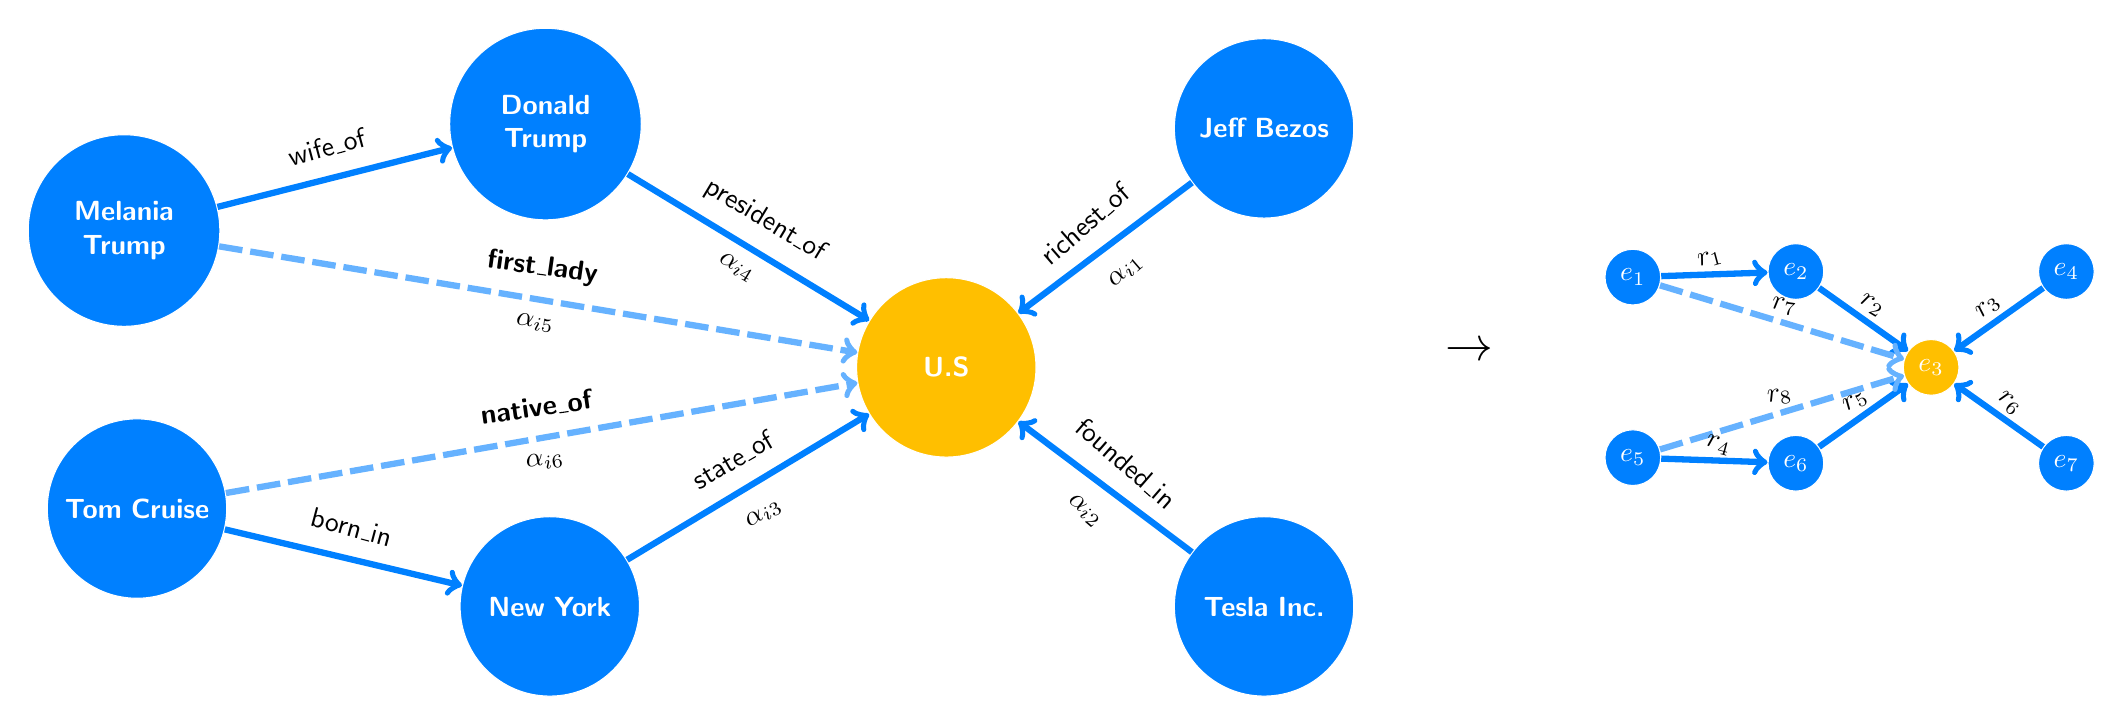
\begin{tikzpicture}[
			entityStyle/.style={draw, color=white, font=\sffamily, thin, align=center, circle, text width=20mm},
			us/.style = {entityStyle, fill=amber},
			entity/.style={entityStyle, fill=azure},
			arrowStyle/.style={-latex', >=stealth, font=\sffamily},
			entityId/.style={draw, color=white, font=\sffamily, thin, align=center, circle},]
			
			\node[us] (us) {\textbf{U.S}};
			
			\begin{scope}[every node/.style={entity}]
				\node[above left=2cm of us, xshift=-20mm] (c1) {\textbf{Donald Trump}};
				\node[above right=2cm of us, xshift=1cm] (c2) {\textbf{Jeff Bezos}};
				\node[below left=2cm of us, xshift=-20mm] (c3) {\textbf{New York}};
				\node[below right=2cm of us, xshift=1cm] (c4) {\textbf{Tesla Inc.}};
				
				\node[below left=3cm of c1, yshift=25mm, xshift=-15mm] (c1x) {\textbf{Melania Trump}};
				\node[above left=3cm of c3, yshift=-25mm, xshift=-15mm] (c3x) {\textbf{Tom Cruise}};
				
				%\node[left=1cm of c1x, yshift=25mm, xshift=-15mm] (c8) {\textbf{Thanh}};
			\end{scope}
			
			%\draw[->, line width=0.8mm, azure] (c8) -> (c1x);
			%\path[arrowStyle] (c8)--node[rotate=-31, yshift=4mm]{friend\_of} %node[rotate=-31, yshift=-3mm]{} (c1x);
			
			\foreach \value in {1,...,4}
			\draw[->, line width=0.8mm, azure] (c\value) -> (us);
			\foreach \value in {1,3}
			\draw[->, line width=0.8mm, azure] (c\value x) -> (c\value);
			
			\foreach \value in {1,3}
			\draw[->, line width=0.8mm, azure!60, dash pattern=on 3mm off 1mm, postaction={decorate}] (c\value x) -> (us);
			
			\path[arrowStyle] (c1)--node[rotate=-31, yshift=4mm]{president\_of} node[rotate=-31, yshift=-3mm]{$\alpha_{i4}$} (us);
			
			\path[arrowStyle] (c3)--node[rotate=30, yshift=4mm]{state\_of} node[rotate=30, yshift=-4mm]{$\alpha_{i3}$} (us);
			
			\path[arrowStyle] (c2)--node[rotate=41, yshift=4mm]{richest\_of} node[rotate=41, yshift=-4mm]{$\alpha_{i1}$} (us);
			
			\path[arrowStyle] (c4)--node[rotate=-41, yshift=4mm]{founded\_in} node[rotate=-41, yshift=-4mm]{$\alpha_{i2}$} (us);
			
			\path[arrowStyle] (c1x)--node[rotate=15, yshift=4mm]{wife\_of} (c1);
			\path[arrowStyle] (c3x)--node[rotate=-15, yshift=4mm]{born\_in} (c3);
			
			\path[arrowStyle] (c1x)--node[rotate=-8, yshift=4mm]{\textbf{first\_lady}} node[rotate=-8, yshift=-3mm]{$\alpha_{i5}$} (us);
			\path[arrowStyle] (c3x)--node[rotate=8, yshift=4mm]{\textbf{native\_of}} node[rotate=8, yshift=-3mm]{$\alpha_{i6}$} (us);
			
			%%%%%%%%%%%
			\node[entityId][fill=amber][right=11cm of us] (country) {$e_3$};
			\path[arrowStyle] (us)--node[yshift=2mm]{\LARGE $\rightarrow$} (country);
			
			\begin{scope}[every node/.style={entityId, fill=azure}]
				\node[above left=1cm of country, xshift=-5mm] (c1s) {$e_2$};
				\node[above right=1cm of country, xshift=5mm] (c2s) {$e_4$};
				\node[below left=1cm of country, xshift=-5mm] (c3s) {$e_6$};
				\node[below right=1cm of country, xshift=5mm] (c4s) {$e_7$};
				
				\node[below left=1.5cm of c1s, yshift=15mm, xshift=-5mm] (c1xs) {$e_1$};
				\node[above left=1.5cm of c3s, yshift=-15mm, xshift=-5mm] (c3xs) {$e_5$};
			\end{scope}
			\foreach \value in {1,...,4}
			\draw[->, line width=0.8mm, azure] (c\value s) -> (country);
			\foreach \value in {1,3}
			\draw[->, line width=0.8mm, azure] (c\value xs) -> (c\value s);
			
			\foreach \value in {1,3}
			\draw[->, line width=0.8mm, azure!60, dash pattern=on 3mm off 1mm, postaction={decorate}] (c\value xs) -> (country);
			
			\path[arrowStyle] (c1s)--node[rotate=-31, yshift=2mm]{$r_2$} (country);
			
			\path[arrowStyle] (c3s)--node[rotate=30, yshift=2mm]{$r_5$} (country);
			
			\path[arrowStyle] (c2s)--node[rotate=41, yshift=2mm]{$r_3$} (country);
			
			\path[arrowStyle] (c4s)--node[rotate=-41, yshift=2mm]{$r_6$} (country);
			
			\path[arrowStyle] (c1xs)--node[rotate=15, yshift=2mm]{$r_1$} (c1s);
			\path[arrowStyle] (c3xs)--node[rotate=-15, yshift=2mm]{$r_4$} (c3s);
			
			\path[arrowStyle] (c1xs)--node[rotate=-8, yshift=2mm]{$r_7$} (country);
			\path[arrowStyle] (c3xs)--node[rotate=8, yshift=2mm]{$r_8$} (country);
		\end{tikzpicture}
	}
	\caption{Đồ thị tri thức và các hệ số chú ý chuẩn hóa của thực thể}
	\label{fig:graphExample}
\end{figure}

Với thành công của \textit{cơ chế chú ý đa đỉnh} trong ngôn ngữ tự nhiên, nó còn được nghiên cứu để áp dụng vào các mô hình của xử lý ảnh \cite{ramachandran2019stand}. Chính vì vậy cơ chế chú ý đa đỉnh đã được nghiên cứu để áp dụng vào các mô hình nhúng đồ thị tri thức thay cho phương pháp tính chập như Mạng Đồ Thị Tích Chập (GCNs \cite{kipf2016semi}). Ở phần này chúng tôi sẽ trình bày chi tiết về cách cơ chế chú ý ở \ref{sec:attentionMechanism} được áp dụng vào việc nhúng đồ thị theo phương pháp Mạng Đồ Thị Chú Ý (Graph Attention Network - GAT \cite{velivckovic2017graph}).

Đầu vào của mô hình \textit{mạng đồ thị chú ý} là tập hợp các vector nhúng được khởi tạo ngẫu nhiên theo phân phối chuẩn biểu diễn đặc trưng của từng thực thể (entity) : $\mathbf{E} = \Big\{\overrightarrow{e_1}, \overrightarrow{e_2}, ...,  \overrightarrow{e_{N_e}}\Big\}$. Mục tiêu của mô hình là biến đổi thành ma trận nhúng đầu ra mới $\mathbf{E}'' = \Big\{\overrightarrow{e''_1}, \overrightarrow{e''_2}, ...,  \overrightarrow{e''_{N_e}}\Big\}$ với khả năng tổng hợp thông tin nhúng từ các thực thể lân cận; $\mathbf{E} \in \mathbb{R}^{N_e \times D_{\text{in}}}$ và $\mathbf{E}'' \in \mathbb{R}^{N_e \times D''}$ tương ứng là ma trận nhúng đầu vào và ma trận nhúng đầu ra của của tập hợp thực thể, $N_e$ là kích thước của tập thực thể, $D_{\text{in}}$ và $D''$ tương ứng là số chiều nhúng đầu vào, và số chiều nhúng đầu ra.

Tương tự như cơ chế chú ý đa đỉnh được trình bày ở mục \ref{sec:attentionMechanism}, việc áp dụng của cơ chế chú ý đa đỉnh trên đồ thị tri thức sẽ áp dụng với chính mỗi vector nhúng thực thể giống như \textit{cơ chế tự-chú ý} (self-attention mechanism), mỗi đỉnh sẽ chú ý với tất cả các đỉnh khác trong đồ thị. Tuy nhiên, việc tính hệ số chú ý giữa tất cả các đỉnh với nhau trong đồ thị là không có ý nghĩa nếu không có mối quan giữa chúng và khối lượng tính toán rất lớn, vì vậy mô hình áp dụng cơ chế gọi là \textit{mặt nạ chú ý} (mask attention) bằng cách bỏ đi tất cả những hệ số chú ý không có quan hệ trong đồ thị, đó chính xác là giá trị của lân cận bậc nhất (Định nghĩa \ref{def:firstOrderProximity}) của một đỉnh trong đồ thị. Khi đó $\mathbf{X} = \mathbf{Y} = \mathbf{E}$ (\ref{sec:attentionMechanism}) và hệ số chú ý của của cơ chế mặt nạ chú ý được hiểu là sự quan trọng của một đỉnh $j \in \mathcal{N}_{i}$ đối với đỉnh gốc $i$, với $\mathcal{N}_{i}$ là tập hợp tất cả những hàng xóm của đỉnh $i$ (bao gồm cả $i$). 

Việc áp dụng cơ chế chú ý đa đỉnh (\textit{multi-head attention}) ở \ref{headAttention} vào đồ thị được mô tả như sau :

\begin{equation}
	\label{maskAttention}
	\centering
	{e_{ij}}={f_{\text{mask attention}}(\mathbf{W} \overrightarrow{e_i}, \mathbf{W} \overrightarrow{e_j})}
\end{equation}

trong đó $e_{ij}$ là hệ số chú ý đa đỉnh của một cạnh $(e_i, e_j)$ đối với thực thể gốc $e_i$ trong đồ thị $\mathcal{G}_{\text{know}}$. $\mathbf{W}$ là ma trận trọng số để tham số hóa quá trình biến đổi tuyến tính. $f_{\text{mask attention}}$ là hàm áp dụng cơ chế chú ý.

Trong mô hình GAT, mô hình sẽ đi qua hai quá trình biến đổi vector nhúng $\overrightarrow{e_i}$ của thực thể $e_i$. Toàn bộ mô hình bao gồm hai bước biến đổi, với mỗi bước là một quá trình biến đổi vector nhúng bằng cơ chế chú ý đa đỉnh như sau :
\begin{equation}
	\label{gatProcess}
	\overrightarrow{e_i} \xrightarrow{f_{\text{mask attention}}^{(1)}} \overrightarrow{e'_i} \xrightarrow{f_{\text{mask attention}}^{(2)}} \overrightarrow{e''_i}
\end{equation}

Ở quá trình chú ý đa đỉnh đầu tiên ($f_{\text{mask attention}}^{(1)}$), mô hình sẽ tổng hợp thông tin từ các thực thể lân cận và ghép chồng lên nhau để tạo ra vector $\overrightarrow{e'_i}$, với $\overrightarrow{e'_i} \in \mathbb{R}^{1 \times D'}$ . Ở bước thứ hai ($f_{\text{mask attention}}^{(2)}$), lớp chú ý đa đỉnh đã đỉnh không còn nhạy cảm với quá trình tự-chú ý nên kết quả sẽ được tính \textit{trung bình} thay vì ghép các đỉnh chú ý lại với nhau, vector $\overrightarrow{e'_i}$ tiếp tục được xem là vector nhúng đầu vào để biến đổi thành vector nhúng $\overrightarrow{e''_i}$ cuối cùng với $\overrightarrow{e''_i} \in \mathbb{R}^{1 \times D''}$.

Đầu tiên, giống như cơ chế chú ý \ref{attention}, mỗi vector nhúng sẽ được nhân với một ma trận trọng số $\mathbf{W}_1 \in \mathbb{R}^{D_k \times D_{\text{in}}}$ để thể tham số hóa quá trình biến đổi tuyến tính từng vector nhúng của thực thể từ số chiều $D_{\text{in}}$ lên số chiều $D_k$ có đặc trưng cao hơn :

\begin{equation}
	\overrightarrow{h_i} = \mathbf{W}_{1} \overrightarrow{e_i}
\end{equation}

khi đó $\overrightarrow{e_i} \in \mathbb{R}^{D_{\text{in}} \times 1}
\xrightarrow{} \overrightarrow{h_i} \in \mathbb{R}^{D_k \times 1}$

Sau đó, ta ghép các cặp vector nhúng thực thể vừa biến đổi tuyến tính với nhau để tính hệ số chú ý, hệ số chú ý $e_{ij}$ thể hiện sự quan trọng của đặc trưng cạnh $(e_i, e_j)$ đối với thực thể gốc $e_i$ hay sự quan trọng của một thực thể $e_j$ có quan hệ với thực thể gốc $e_i$ , ta áp dụng hàm $\text{LeakyReLU}$ để lấy giá trị tuyệt đối của hệ số chú ý, mỗi hệ số chú ý $e_{ij}$ được tính theo công thức sau :

\begin{equation}
	e_{ij} = \Big( \text{LeakyReLU} \Big( \overrightarrow{\mathbf{W}_{2}}^{T} [\overrightarrow{h_i} || \overrightarrow{h_j}]\Big) \Big)
\end{equation}

với ${.}^{T}$ là phép chuyển vị, $||$ là phép ghép. Tương tự \ref{attention}, tuy nhiên thay vì thực hiện tính tích vô hướng thì ta sử dụng một \textit{cơ chế chú ý chung} (shared attentional mechanism) $\overrightarrow{\mathbf{W}_2}$ : $\mathbb{R}^{D_k} \times \mathbb{R}^{D_k} \xrightarrow{} \mathbb{R}$ để tính hệ số chú ý. Như đã trình bày ở \ref{maskAttention}, ta thực hiện tự chú ý giữa tất cả các đỉnh với nhau bằng cơ chế mặt nạ chú ý để bỏ hết tất cả thông tin cấu trúc.
Để có thể dễ dàng so sánh các hệ số chú ý với nhau giữa tất cả các thực thể, một hàm \textit{softmax} được áp dụng để chuẩn hóa trên tất cả các hàng xóm $e_j$ có quan hệ với thực thể gốc $e_i$ : $\alpha_{ij} = \text{softmax}_j(e_{ij})$. Kết hợp lại ta có công thức của hệ số chú ý chuẩn hóa của từng hàng xóm đối với thực thể gốc như sau :

\begin{equation}
	\label{attentionCoeff}
	\alpha_{ij} = \frac{
		\text{exp} \Big( \text{LeakyReLU} \Big( \overrightarrow{\mathbf{W}_2}^{T} [ \overrightarrow{h_i} || \overrightarrow{h_j}]\Big) \Big))
	}
	{
		\sum_{k \in \mathcal{N}_i}
		\text{exp} \Big( \text{LeakyReLU} \Big( \overrightarrow{\mathbf{W}_2}^{T} [\overrightarrow{h_i} || \overrightarrow{h_k}]\Big) \Big))
	}
\end{equation}

Ở bước này, mô hình GAT tương tự như GCN \cite{kipf2016semi}, các vector nhúng từ hàng xóm sẽ được tổng hợp với nhau và mở rộng hay thu nhỏ (scale) theo hệ số chú ý đã chuẩn hóa :

\begin{equation}
	\label{scaleAttentionCoef}
	\centering
	{\overrightarrow{e'_i}}={\sigma\left(\sum_{j\in \mathcal{N}_i} {\alpha_{ij} \overrightarrow{h_j} }\right)}
\end{equation}

Tương tự như lớp chú ý đa đỉnh, ta sẽ ghép $N_{\text{head}}$ đỉnh lại với nhau để giúp ổn định quá trình học ở bước ($f_{\text{mask attention}}^{(1)}$ \ref{gatProcess}) đầu tiên của mô hình:

\begin{equation}
	\label{multiHeadAttention}
	{\overrightarrow{e'_i}}={\bigparallel_{h=1}^{N_{\text{head}}}\sigma\left(\sum_{j\in \mathcal{N}_i}\alpha_{ij}^{h} \mathbf{W}^{h} \overrightarrow{h_{j}} \right)}
\end{equation}

trong đó $\sigma$ là bất kỳ hàm biến đổi phi tuyến tính nào, $\alpha_{ij}^h$ là hệ số chú ý được chuẩn hóa của cạnh $(e_i, e_j)$ được tính từ lớp thứ $h^{th}$, tương tự như công thức \ref{attention} $\mathbf{W}^h$ là ma trận trọng số để biến đổi tuyến tính vector nhúng đầu vào, với $\mathbf{W}^h$ thuộc các lớp ghép chồng $h^{th}$ khác nhau. Cuối cùng vector nhúng mới $\overrightarrow{e'_i} \in \mathbb{R}^{1 \times D'}$ với $D' = N_{\text{head}} D_{\text{k}}$ tiếp tục được xem là vector đầu vào để thực hiện cơ chế chú ý. Tuy nhiên ở bước thứ hai ($f_{\text{mask attention}}^{(2)}$ \ref{gatProcess}) giá trị chú ý đa đỉnh sẽ được tính trung bình thay vì ghép chồng lên nhau theo công công thức sau :

\begin{equation}
	\label{multiHeadConcat}
	{\overrightarrow{e''_i}}={\sigma\left(\frac{1}{N_{\text{head}}} \sum_{h=1}^{N_{\text{head}}}\sum_{j\in \mathcal{N}_i}\alpha_{ij}^{h} \mathbf{W}^{h} \overrightarrow{e'_{j}} \right)}
\end{equation}

\textbf{Tổng kết} : Đến đây chúng tôi đã trình bày được cách cơ chế chú ý tổng hợp một vector nhúng thực thể trong đồ thị tri thức từ các vector nhúng lân cận và ghép lại với nhau để tạo ra vector nhúng kết quả. Trong phần tiếp theo chúng tôi sẽ trình bày đầy đủ về mô hình nhúng của chúng tôi dựa trên mô hình KBGAT của nhóm tác giả Nathani, Deepak\cite{nathani2019learning} .

\section{Mô hình KBGAT}

Trong đồ thị tri thức, một thực thể không thể là một đại diện đầy đủ cho một cạnh, vì một thực thể có thể đóng nhiều vai trò khác nhau phụ thuộc vào từng loại quan hệ khác nhau. Ví dụ như hình \ref{fig:graphExample}, Donald Trump vừa đóng là vai trò là tổng thống, vừa đóng vai trò là người chồng. Để giải quyết vấn đề này, mô hình nhúng đồ thị dựa trên chú ý - KBGAT (graph attention based embeddings \cite{nathani2019learning}) là một cải tiến của mô hình GAT bằng cách kết hợp thêm thông tin của \textit{quan hệ và đặc trưng các đỉnh hàng xóm} vào trong cơ chú ý. Trong phần này chúng tôi sẽ trình bày chi tiết về mô hình KBGAT. Cấu trúc của KBGAT là một mô hình mã hóa-giải mã (encoder-decoder) trong đó lớp mã hóa chúng tôi sử dụng mô hình Mạng đồ thị chú ý, còn với mô hình giải mã chúng tôi sử dụng mô hình ConvKB để tiến hành dự đoán. Các bước của mô hình KBGAT được minh họa ở \ref{eq:KBGATProcess}.

\begin{equation}
	\label{eq:KBGATProcess}
	entities \xrightarrow{\text{Embedding}^{\ref{sec:initTransE}}} \overrightarrow{e_{\text{TransE}}} \xrightarrow{\text{Embedding} ^{\ref{sec:encodeKBGAT}}} \overrightarrow{e_{\text{KBGAT}}} \xrightarrow{\text{ConvKB}^{\ref{sec:predictionConvKB}}} e_{\text{prob}}
\end{equation}

Đầu tiên, các vector nhúng của mỗi thực thể được khởi tạo bằng mô hình TransE để học được các đặc trưng không gian giữa các đỉnh để thu được vector nhúng. 
Sau đó các vector nhúng này được tiếp tục huấn luyện bằng mô hình mã hóa để học được các đặc trưng lân cận để có được vector nhúng mới. Cuối cùng, các vector nhúng này đi qua lớp dự đoán bằng mô hình ConvKB. Tất cả các công thức của chúng tôi đều được trình bày lại theo nhóm tác giả Nathani, Deepak\cite{nathani2019learning}.

\subsection{Khởi tạo vector nhúng}
\label{sec:initTransE}

\begin{figure}[htp]
	\centering
	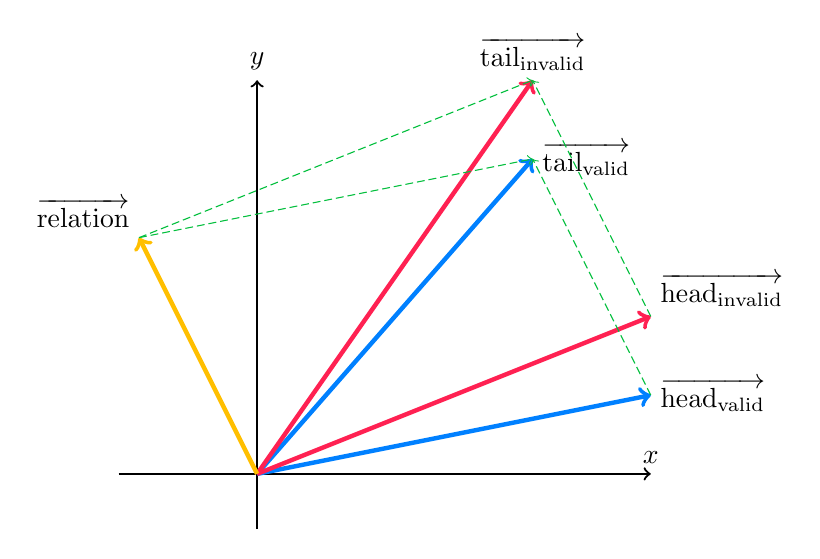
\begin{tikzpicture}[
		arrow/.style={->,thick},
		vector/.style={arrow, ultra thick},
		dashLine/.style={->, thin, dash pattern=on 1mm off 0.5mm},
		formal/.style={font=\sffamily}]
		\coordinate (root) at (0,0);
		\coordinate [formal, label=above left:$\overrightarrow{\text{relation}}$] (c1) at (-1.5, 3);
		\coordinate [formal, label=above:$\overrightarrow{\text{tail}_{\text{invalid}}}$] (c2) at (3.5, 5);
		\coordinate [formal, label=right:$\overrightarrow{\text{tail}_{\text{valid}}}$] (c3) at (3.5, 4);
		\coordinate [formal, label=above right :$\overrightarrow{\text{head}_{\text{invalid}}}$] (c4) at (5, 2);
		\coordinate [formal, label=right:$\overrightarrow{\text{head}_{\text{valid}}}$] (c5) at (5, 1);
		
		\draw [arrow] ([yshift=-2em] root) -> (0, 5) node (yaxis)[above] {$y$};
		\draw [arrow] ([xshift=-5em] root) -> (5, 0) node (xaxis)[above] {$x$};
		
		\foreach \x in {3, 5}
		{\draw [vector, color=azure] (root) -> (c\x);}
		
		\foreach \x in {2, 4}
		{\draw [vector, color=awesome] (root) -> (c\x);}
		
		\draw [vector, color=amber] (root) -> (c1);
		
		\foreach \x in {1, 4}
		{\draw [dashLine, color=darkpastelgreen] (c\x) -> (c2);}
		
		\foreach \x in {1, 5}
		{\draw [dashLine, color=darkpastelgreen] (c\x) -> (c3);}
	\end{tikzpicture}
	\caption{Minh họa về các vector nhúng trong mô hình TransE}
	\label{fig:TransEAnimation}
\end{figure}

Tương tự như phương pháp Word2Vec\cite{mikolov2013efficient}, mô hình \textit{Biến đổi vector nhúng để mô hình hóa dữ liệu đa-quan hệ} (TransE \cite{bordes2013translating}) thuộc nhóm các phương pháp nhúng hình học để biến đổi các thực thể và quan hệ trong đồ thị tri thức thành các vector nhúng đầu ra sao cho :
\begin{equation}
	\label{eq:conditionTransE}
	\overrightarrow{\text{entity}_{\text{head}}} + \overrightarrow{relation} \approx \overrightarrow{\text{entity}_{\text{tail}}}
\end{equation}

Đầu tiên, các vector nhúng thực thể và quan hệ được khởi tạo ngẫu nhiên bằng phân phối chuẩn theo số chiều của vector khởi tạo $D_{\text{in}}$, sau đó được chuẩn hóa theo kích thước của tập thực thể nhúng, và quan hệ nhúng.
Sau đó, ta lấy mẫu (sampling) từ tập dữ liệu huấn luyện để có được một \textit{lô bộ ba hợp lệ} ($S_{\text{batch}}$). Với mỗi bộ ba như vậy, chúng ta lấy mẫu bộ ba không hợp lệ bằng cách thay thực thể đầu hoặc thực thể đuôi bằng một thực thể ngẫu nhiên trong tập thực thể để được \textit{lô bộ ba không hợp lệ} ($S'_{\text{batch}}$). Sau đó ta nhóm từng bộ ba hợp lệ với không hợp lệ để tạo ra \textit{lô huấn luyện} ($T_{\text{batch}}$). Cuối cùng, ta cập nhật giá trị các vector nhúng để đảm bảo điều kiện  \ref{eq:conditionTransE} .

\begin{algorithm}
	\caption{Thuật toán học vector nhúng TransE \protect\cite{bordes2013translating}}\label{alg:TransE}
	\begin{algorithmic}[1]
		\Statex \textbf{Input} :
		Tập huấn luyện $S = {(h, r, t)}$, tập thực thể E, tập quan hệ R, biên lề $\gamma$, số chiều nhúng $D_{\text{in}}$	
		\Statex \textbf{Initialize}
		\State $\overrightarrow{r} \leftarrow \text{uniform}(-\frac{6}{\sqrt{D_{\text{in}}}}, \frac{6}{\sqrt{D_{\text{in}}}})$ với mỗi quan hệ $r \in R$
		\State $\overrightarrow{r} \leftarrow \frac{\overrightarrow{r}}{\|\overrightarrow{r}\|}$ với mỗi $r \in R$
		\State $\overrightarrow{e} \leftarrow \text{uniform}(-\frac{6}{\sqrt{D_{\text{in}}}}, \frac{6}{\sqrt{D_{\text{in}}}})$ với mỗi thực thể $e \in E$
		\Loop
		\State $\overrightarrow{e} \leftarrow \frac{\overrightarrow{e}}{\|\overrightarrow{e}\|}$ với mỗi $e \in E$
		\State $S_{\text{batch}} \leftarrow \text{sample}(S, b)$  // lấy mẫu minibatch kích thước $b$
		\State $T_{\text{batch}} \leftarrow \varnothing $
		\For {$(h, r, t) \in S_{\text{batch}}$}
		\State $(h', r, t') \leftarrow \text{sample}(S'_{(h, r, t)})$ // lấy mẫu từ bộ ba không hơp lệ
		\State $T_{\text{batch}} \leftarrow T_{\text{batch}} \cup \Big\{ \Big( (h, r, t), (h', r, t') \Big) \Big\}$
		\EndFor
		\Statex Cập nhật nhúng
		\State $\sum_{\Big( (h, r, t), (h', r, t')\Big) \in T_{\text{batch}}} \nabla [\gamma + d(\overrightarrow{h} + \overrightarrow{r}, \overrightarrow{t}) - d(\overrightarrow{h'} + \overrightarrow{r}, \overrightarrow{t'})]_{+}$
		\EndLoop
		\Statex \textbf{Output} :
		tập các vector có số chiều là $D_{\text{in}}$ đại điện cho các thực thể và quan hệ
	\end{algorithmic}
\end{algorithm}

Mô hình TransE của nhóm tác giả Bordes, Antoine\cite{bordes2013translating} được trình bày ở thuật toán \ref{alg:TransE}.

Trong đó, đầu vào của mô hình TransE là tập dữ liệu huấn luyện với mỗi phần tử là một bộ ba $(h, r, t)$. $h, t \in E$ là các thực thể đầu và thực thể đuôi, $r \in R$ là các quan hệ.$\overrightarrow{e}$ và $\overrightarrow{r}$ lần lượt là các vector nhúng của thực thể và quan hệ, và $\|\overrightarrow{e}\|$ và $\|\overrightarrow{r}\|$ lần lượt là độ lớn của tập thực thể và tập quan hệ. $S$ và $S_{\text{batch}}$ tương ứng là tập dữ liệu huấn luyện, và một lô (batch) lấy ra từ tập dữ liệu huấn luyện.
$T_{\text{batch}}$ là một lô bao gồm cả bộ ba hợp lệ và bộ ba không hợp lệ để tính hàm mất mát \ref{eq:sampleTransE} .

\textit{Bộ ba hợp lệ} (valid triple) là bộ ba lấy từ lô huấn luyện ($S_{\text{batch}}$), \textit{bộ ba không hợp lệ} (invalid triple) là bộ ba lấy từ lô huấn luyện lỗi ($S'_{\text{batch}}$) được bỏ đi thực thể đầu hoặc thực thể đuôi và thay thế các thực thể đó bằng cách chọn một thực thể ngẫu nhiên trong tập thực thể :

\begin{equation}
	\label{eq:sampleTransE}
	\centering
	S'_{(h, r, t)} = \big\{ (h', r, t) | h' \in E \big\} \cup \big\{ (h, r, t') | t' \in E \big\}
\end{equation}

Để đạt được mục tiêu là tạo ra các vector nhúng sao cho $\overrightarrow{h} + \overrightarrow{r} \approx \overrightarrow{t}$, ý tưởng của mô hình là các vector nhúng trong lô hợp lệ thì vector nhúng đuôi $\overrightarrow{t}$ phải ở lân cận của $\overrightarrow{h} + \overrightarrow{r}$, ngược lại các vector nhúng trong lô không hợp lệ $\overrightarrow{h'} + \overrightarrow{r}$ (hoặc $\overrightarrow{t'}$) thì phải nằm xa so với $\overrightarrow{t}$ (hoặc $\overrightarrow{h} + \overrightarrow{r}$) theo hàm mất mát sau :

\begin{equation}
	\label{eq:KBGATLoss}
	\centering
	\mathcal{L} = \sum_{(h, r, t) \in S} \sum_{(h', r, t') \in S'_{(h, r, t)}} [d - d' + \gamma]_{+}
\end{equation}

\begin{figure}[htp]
	\centering
	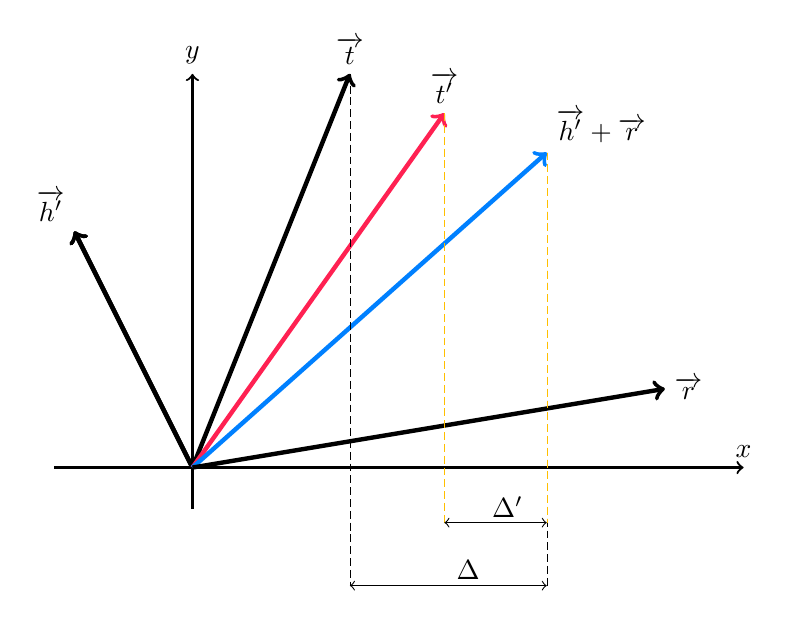
\begin{tikzpicture}[
		arrow/.style={->,thick},
		vector/.style={arrow, ultra thick},
		mapping/.style={->, thin},
		distArrow/.style={thin, <->},
		dashLine/.style={very thin, dash pattern=on 1mm off 0.5mm},
		formal/.style={font=\sffamily}]
		
		\coordinate (root) at (0,0);
		\coordinate [formal, label=above left:$\overrightarrow{h'}$] (c1) at (-1.5, 3);
		\coordinate [formal, label=above:$\overrightarrow{t}$] (c2) at (2, 5);
		\coordinate [formal, label=above:$\overrightarrow{t'}$] (c3) at (3.2, 4.5);
		\coordinate [formal, label=above right :$\overrightarrow{h'} + \overrightarrow{r}$] (c4) at (4.5, 4);
		\coordinate [formal, label=right:$\overrightarrow{r}$] (c5) at (6, 1);
		
		\draw [arrow] ([yshift=-1.5em] root) -> (0, 5) node (yaxis)[above] {$y$};
		\draw [arrow] ([xshift=-5em] root) -> (7, 0) node (xaxis)[above] {$x$};
		
		\foreach \x in {1, 5}
		{\draw [vector, color=black] (root) -> (c1);}
		{\draw [vector, color=black] (root) -> (c2);}
		{\draw [vector, color=awesome] (root) -> (c3);}
		{\draw [vector, color=azure] (root) -> (c4);}
		{\draw [vector, color=black] (root) -> (c5);}
		
		\draw [dashLine] (c2) -> (2, -1.5) node (mapc2){};
		\draw [dashLine] (c4) -> (4.5, -1.5) node (mapc4){};
		
		\draw [dashLine, color=amber] (c3) -> (3.2, -0.7) node (mapc3){};
		\draw [dashLine, color=amber] (c4) -> (4.5, -0.7) node (mapc4){};
		
		\draw [distArrow] (2, -1.5) node (map1c2) {} -> (3.5, -1.5) node (alpha)[yshift=2mm] {$\Delta$} -> (4.5, -1.5) node (mapc4){};
		\draw [distArrow] (3.2, -0.7) node (map1c3) {} -> (4, -0.7) node (alpha)[yshift=2mm] {$\Delta'$} ->  (4.5, -0.7) node (mapc4){};
	\end{tikzpicture}
	\caption{Minh học về độ đo hàm loss trong TransE}
	\label{fig:TransEExplain}
\end{figure}

Với $\gamma > 0$ là biên lề, $h'$ và $t'$ lần lượt là các thực thể lấy mẫu trong công thức \ref{eq:sampleTransE} ; $\Delta$ và $\Delta'$ lần lượt là hàm đo giá trị sai khác của các thực thể nhúng trong lô hợp lệ $d = \big\|\Delta \big\|_{1}  = \big\| \overrightarrow{h} + \overrightarrow{r} - \overrightarrow{t}\big\|_{1}$ và lô không hợp lệ $d' = \big\|\Delta' \big\|_{1} = \big\| \overrightarrow{h'} + \overrightarrow{r} - \overrightarrow{t'}\big\|_{1}$ ($\|\|_{1}$ là hàm chuẩn hóa L1-norm) .
Theo minh họa trong \figurename{ } \ref{fig:TransEExplain}, ta thấy nếu $d > d'$ hay $d - d' > 0$ thì $\overrightarrow{h} + \overrightarrow{r}$ sẽ nằm gần $\overrightarrow{\text{t}}$ hơn so với $\overrightarrow{t'}$. Ta muốn các vector nhúng thõa mãn điều kiện \ref{eq:conditionTransE} nên $\overrightarrow{h} + \overrightarrow{r}$ phải càng gần $t$ càng tốt, nghĩa là $\overrightarrow{h} + \overrightarrow{r}$ càng gần $\overrightarrow{t'}$ thì càng không đúng. Vì vậy trong quá trình huấn luyện ta muốn $\Delta'$ càng lớn bằng $\Delta$ càng tốt và nếu $\Delta' > \Delta$ hay $d' - d > 0$ thì ta không cần cập nhật các trọng số nhúng nữa. Vì vậy trong hàm mất mát \ref{eq:KBGATLoss} $[d - d' + \gamma]_{+}$ là ta muốn lấy phần dương vì phần âm đã đảm bảo tính đúng đắn của điều kiện \ref{eq:conditionTransE} trong quá trình huấn luyện.

\subsection{Mô hình mã hóa}
\label{sec:encodeKBGAT}

Sau khi có được các vector nhúng học được các đặc trưng không gian ở trên của đồ thị. Các vector nhúng tiếp tục được đi qua lớp nhúng tiếp theo để tổng hợp thêm thông tin lân cận của một thực thể.

\begin{figure}[htp]
	\centering
	\resizebox{\textwidth}{!}{%
		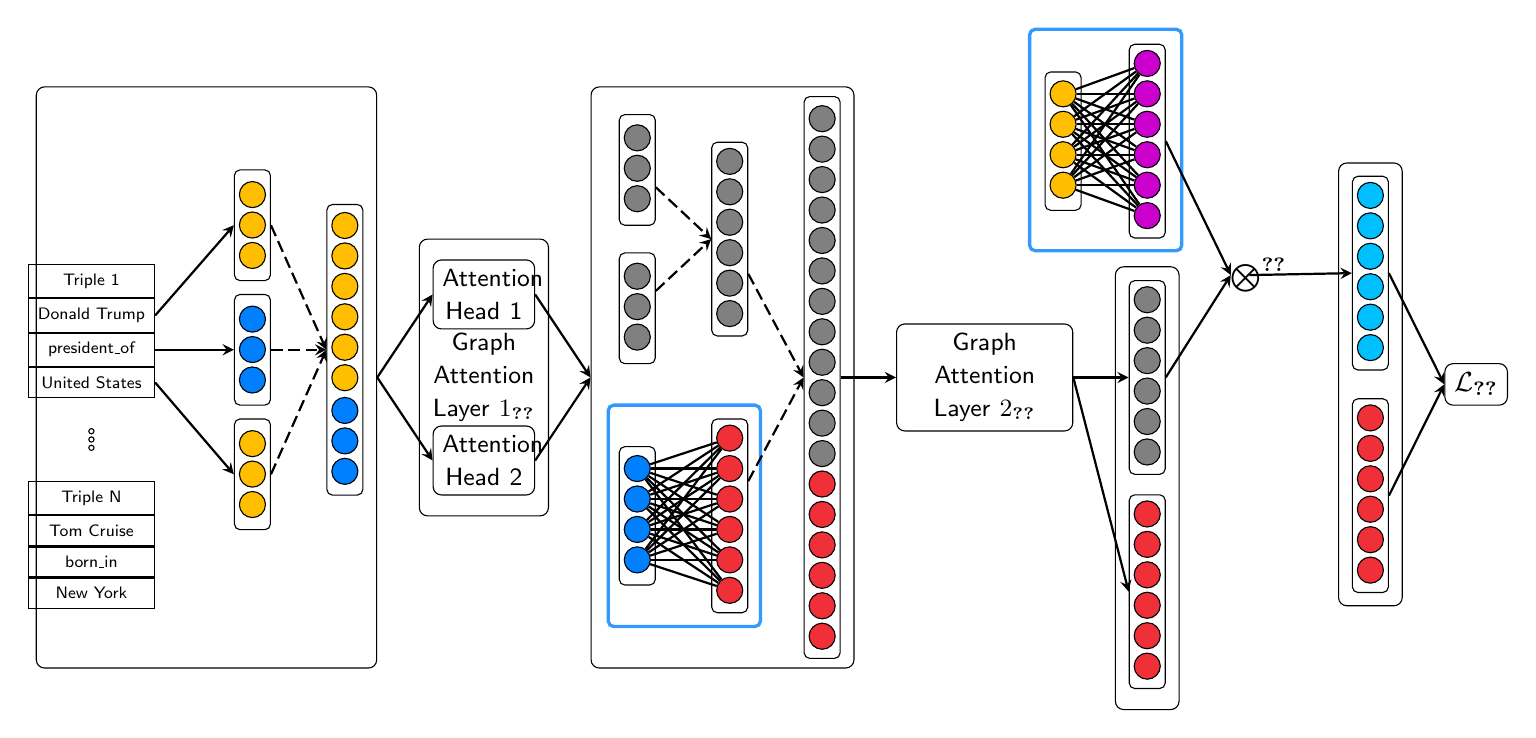
\begin{tikzpicture}[
			emb/.style={draw, circle,minimum width=.1em, thin, anchor=center},
			entityInit/.style={emb, fill=amber},
			relationInit/.style={emb, fill=azure},
			entityEmb/.style={emb, fill=gray},
			relationEmb/.style={emb, fill=deepcarminepink},
			entityPretrain/.style={emb, fill=deepmagenta},
			entityOut/.style={emb, fill=deepskyblue},
			box/.style={draw,rectangle, fill=none},
			embBox/.style={box ,rounded corners=0.2em, minimum width=1.3em},
			layerBox/.style={color=azure!80, box ,very thick,rounded corners=0.2em, minimum width=1.3em},
			textbox/.style={box,rounded corners=0.3em, fill=none,font=\sffamily, align=center},
			arrowStrong/.style={thick,->,>=stealth},
			arrowDash/.style={thick, ->,>=stealth, dash pattern=on 1.5mm off 0.7mm, postaction={decorate}},
			row/.style={draw, rectangle, font=\fontsize{0.6em}{1}\sffamily, align=center, text width=3.9em},
			arrowStyle/.style={-latex', font=\sffamily},
			mydot/.style={draw, circle, minimum size=0.1em, scale=0.2},
			]
			% 5
			% Root
			\draw node[textbox][text width=5.7em] (graphAttention2) {\small Graph Attention Layer $2_{\ref{eq:graphAttention2}}$};
			
			\draw node[textbox][minimum width=9.5em, minimum height=21em, left=1.5em of graphAttention2] (layer3) {};
			
			\draw node[embBox][minimum height=20.3em, left=2em of graphAttention2] (box10) {};
			\begin{scope}[every node/.style={below=0mm of box10.center}]
				\foreach \x in {1,...,12}
				{\draw node[entityEmb][yshift=(\x-4)*1.1em+0.55em] (ex10\x) {};}
				
				\foreach \x in {1,...,6}
				{\draw node[relationEmb](ey10\x)[yshift=-(\x+3)*1.1em+0.55em]{};}
			\end{scope}
			
			\draw node[embBox][minimum height=7em, left=2em of box10, yshift=5em] (box7) {};
			\draw node[embBox][minimum height=7em, left=2em of box10, yshift=-5em] (box9) {};
			\begin{scope}
				\foreach \x in {1,...,6}
				{\draw node[entityEmb](e7\x)[yshift=(\x-3)*1.1em, below=0mm of box7.center]{};}
				
				\foreach \x in {1,...,6}
				{\draw node[relationEmb](e9\x)[yshift=(\x-3)*1.1em, below=0mm of box9.center]{};}
			\end{scope}
			
			\draw node[embBox][minimum height=4em, left=2em of box7, yshift=2.5em] (box5) {};
			\draw node[embBox][minimum height=4em, left=2em of box7, yshift=-2.5em] (box6) {};
			\draw node[embBox][minimum height=5em, left=2em of box9] (box8) {};
			\begin{scope}
				\foreach \x in {1,...,3}
				{\draw node[entityEmb](e5\x)[yshift=(\x-2)*1.1em+0.55em, below=0mm of box5.center]{};}
				
				\foreach \x in {1,...,3}
				{\draw node[entityEmb](e6\x)[yshift=-(\x-2)*1.1em+0.55em, below=0mm of box6.center]{};}
				
				\foreach \x in {1,...,4}
				{\draw node[relationInit](e8\x)[yshift=(\x-2)*1.1em, below=0mm of box8.center]{};}
			\end{scope}
			\draw node[layerBox][minimum height=8em,minimum width=5.5em, left=1.5em of box10, yshift=-5em] (fc1) {};
			
			% Left
			\begin{scope}[every node/.style={left=2em of layer3}]
				\draw node[textbox][yshift=3em, text width=3em] (attentionHead1) {\small Attention Head 1};
				\draw node[textbox][yshift=-3em, text width=3em] (attentionHead2) {\small Attention Head 2};
			\end{scope}
			\draw node[textbox][left=1.5em of layer3, text width=4em, minimum width=4em, minimum height=10em] (graphAttention1) {\small Graph Attention Layer $1_{\ref{eq:graphAttention1}}$ };
			
			\draw node[textbox][minimum width=12.3em, minimum height=21em, left=1.5em of graphAttention1] (layer1) {};
			% Layer 1
			\draw node[embBox][minimum height=10.5em, yshift=1em,right=3em of layer1.center, left=2em of graphAttention1] (box4) {};
			\begin{scope}
				\foreach \x in {1,...,6}
				{\draw node[entityInit](ex4\x)[yshift=(\x-2)*1.1em-0.4em, above=0em of box4.center]{};}
				
				\foreach \x in {1,...,3}
				{\draw node[relationInit](e4y\x)[yshift=-(\x)*1.1em-0.6em, below=0mm of box4.center]{};}
			\end{scope}
			
			% Start Initial
			\draw node[embBox][minimum height=4em, yshift=4.5em, left=2em of box4] (box1) {};
			\foreach \x in {1,...,3}
			{\draw node[entityInit](e1\x)[yshift=(\x-2)*1.1em+0.5em, below=0mm of box1.center]{};}
			
			\draw node[embBox][minimum height=4em, left=2em of box4] (box2) {};
			\foreach \x in {1,...,3}
			{\draw node[relationInit](e2\x)[yshift=(\x-2)*1.1em+0.5em, below=0mm of box2.center]{};}
			
			\draw node[embBox][minimum height=4em, yshift=-4.5em, left=2em of box4] (box3) {};
			\foreach \x in {1,...,3}
			{\draw node[entityInit](e3\x)[yshift=(\x-2)*1.1em+0.5em, below=0mm of box3.center]{};}
			% Start Initial
			
			\begin{scope}[every node/.style={left=of box2, row}]
				\draw node (relation1) {president\_of};
				\draw node[above=0mm of relation1] (entity1) {Donald Trump};
				\draw node[above=0mm of entity1] (triple1) {Triple 1};
				\draw node[below=0mm of relation1] (entity2) {United States};	
			\end{scope}
			
			\begin{scope}[every node/.style={row}]
				\draw node[below=3em of entity2] (triple2) {Triple N};
				\draw node[below=0mm of triple2] (entity3) {Tom Cruise};
				\draw node[below=0mm of entity3] (relation2) {born\_in};
				\draw node[below=0mm of relation2] (entity4) {New York};	
			\end{scope}
			
			% Right
			\draw node[textbox][minimum height=16em, minimum width=2.3em, yshift=-4em, right=1.5em of graphAttention2] (layer4){};
			\draw node[embBox][minimum height=7em, right=2em of graphAttention2] (box11) {};
			\begin{scope}
				\foreach \x in {1,...,6}
				{\draw node[entityEmb](e11\x)[yshift=(\x-3)*1.1em, below=0mm of box11.center]{};}
			\end{scope}
			
			\draw node[embBox][minimum height=7em, below=0.7em of box11] (box12) {};
			\begin{scope}
				\foreach \x in {1,...,6}
				{\draw node[relationEmb](e12\x)[yshift=(\x-3)*1.1em, below=0mm of box12.center]{};}
			\end{scope}
			
			\draw node[embBox][minimum height=7em, above=1.5em of box11] (box13) {};
			\begin{scope}
				\foreach \x in {1,...,6}
				{\draw node[entityPretrain](e13\x)[yshift=(\x-3)*1.1em, below=0mm of box13.center]{};}
			\end{scope}
			
			\draw node[embBox][minimum height=5em, left=1.7em of box13] (box14) {};
			\begin{scope}
				\foreach \x in {1,...,4}
				{\draw node[entityInit](e14\x)[yshift=(\x-2)*1.1em, below=0mm of box14.center]{};}
			\end{scope}
			\draw node[layerBox][minimum height=8em, minimum width=5.5em, above=1.5em of box11, yshift=-0.5em, xshift=-1.5em] (fc2) {};
			
			\draw node[right=2em of box11, yshift=3.7em] (bigOTimes) {$\bigotimes^{\ref{eq:reInitEmbedding}}$};
			
			\draw node[textbox][minimum height=16em, minimum width=2.3em, yshift=-3.95em, right=1.5em of bigOTimes] (layer5) {};
			\draw node[embBox][minimum height=7em, above=1em of layer5.center, yshift=-0.5em] (box15) {};
			\begin{scope}
				\foreach \x in {1,...,6}
				{\draw node[entityOut](e15\x)[yshift=(\x-3)*1.1em, below=0mm of box15.center]{};}
			\end{scope}
			
			\draw node[embBox][minimum height=7em, below=1em of layer5.center, yshift=0.5em] (box16) {};
			\begin{scope}
				\foreach \x in {1,...,6}
				{\draw node[relationEmb](e16\x)[yshift=(\x-3)*1.1em, below=0mm of box16.center]{};}
			\end{scope}
			
			\draw node[textbox][right=1.5em of layer5] (final) {$\mathcal{L}_{\ref{eq:KBGATLoss}}$};
			%16
			% Arrow
			\draw [arrowStrong] (box10) -- (graphAttention2.west);
			
			\draw [arrowStrong] (entity1.east) -- (box1.west);
			\draw [arrowStrong] (relation1) -- (box2.west);
			\draw [arrowStrong] (entity2.east) -- (box3.west);
			
			\draw [arrowStrong] (graphAttention2.east) -- (box11.west);
			\draw [arrowStrong] (graphAttention2.east) -- (box12.west);
			
			\draw [arrowStrong] (box11.east) to ([xshift=0.35em] bigOTimes.west);
			\draw [arrowStrong] (box13.east) to ([xshift=0.35em] bigOTimes.west);
			
			\draw [arrowStrong] ([xshift=-1.7em] bigOTimes.east) -- (box15.west);
			
			\draw [arrowStrong] (box16.east) -- (final.west);
			\draw [arrowStrong] (box15.east) -- (final.west);
			
			\foreach \x in {1,2}
			\draw [arrowStrong] (layer1.east) -- (attentionHead\x.west);
			
			\foreach \x in {1,2}
			\draw [arrowStrong] (attentionHead\x.east) -- (layer3.west);
			
			\foreach \x in {1,2,3}
			\draw [arrowDash] (box\x.east) -- (box4.west);
			
			\foreach \x in {7,9}
			{\draw [arrowDash] (box\x) -- (box10.west);}
			
			\foreach \x in {5,6}
			{\draw [arrowDash] (box\x) -- (box7.west);}
			
			\foreach \x in {1, ..., 6}
			{\draw [thick] (e81) -- (e9\x);}
			\foreach \x in {1, ..., 6}
			{\draw [thick] (e82) -- (e9\x);}
			\foreach \x in {1, ..., 6}
			{\draw [thick] (e83) -- (e9\x);}
			\foreach \x in {1, ..., 6}
			{\draw [thick] (e84) -- (e9\x);}
			
			\foreach \x in {1, ..., 6}
			{\draw [thick] (e141) -- (e13\x);}
			\foreach \x in {1, ..., 6}
			{\draw [thick] (e142) -- (e13\x);}
			\foreach \x in {1, ..., 6}
			{\draw [thick] (e143) -- (e13\x);}
			\foreach \x in {1, ..., 6}
			{\draw [thick] (e144) -- (e13\x);}
			
			\draw node[mydot][below=1.1em of entity2] (dot1) {};
			\draw node[mydot][below=1.4em of entity2] (dot2) {};
			\draw node[mydot][below=1.7em of entity2] (dot3) {};
		\end{tikzpicture}
	}
	\caption{Minh họa các lớp mã hóa của mô hình KBGAT}
	\label{fig:encoderKBGAT}
\end{figure}

Mô hình sẽ biến đổi từ ma trận nhúng thực thể

$\mathbf{E} = \Big\{\overrightarrow{e_1}, \overrightarrow{e_2}, ...,  \overrightarrow{e_{N_e}}\Big\} \xrightarrow{} \mathbf{E''} = \Big\{\overrightarrow{e''_1}, \overrightarrow{e''_2}, ...,  \overrightarrow{e''_{N_e}}\Big\}$, với $\mathbf{E} \in \mathbb{R}^{N_e \times D_{\text{in}}}$ và $\mathbf{E''} \in \mathbb{R}^{N_e \times D''}$.
Đồng thời biến đổi ma trận nhúng quan hệ 
$\mathbf{R} = \Big\{\overrightarrow{r_1}, \overrightarrow{r_2}, ...,  \overrightarrow{r_{N_r}}\Big\} \xrightarrow{} \mathbf{R''} = \Big\{\overrightarrow{r''_1}, \overrightarrow{r''_2}, ...,  \overrightarrow{r''_{N_r}}\Big\}$ với $\mathbf{R} \in \mathbb{R}^{N_r \times P_{\text{in}}}$ và $\mathbf{R''} \in \mathbb{R}^{N_r \times P''}$. Tương tự như mô hình GAT đã trình bày ở mục \ref{sec:GAT}, mô hình sẽ biến đổi vector nhúng thực thể $D_{\text{in}}$ chiều thành $D''$ chiều với thông tin được tổng hợp từ các hệ số chú ý lân cận. $P_{\text{in}}$ và $P''$ lần lượt là số chiều của vector nhúng quan hệ đầu vào và đầu ra. $N_e$, $N_r$ tương ứng là kích thước của tập thực thể và tập quan hệ trong $\mathcal{G}_{know}$.

Mô hình KBGAT sẽ ghép các vector nhúng thực thể và vector nhúng quan hệ theo cấu trúc như sau :

\begin{equation}
	\label{attentionWithRelation}
	\overrightarrow{t_{ijk}} = \mathbf{W_1} [\overrightarrow{e_i} || \overrightarrow{e_j} || \overrightarrow{r_k}]
\end{equation}

Với $\overrightarrow{t_{ijk}}$ là vector nhúng đại diện cho bộ ba  $t_{ij}^k = (e_i, r_k, e_j)$ với $e_j$, và $r_k$ lần lượt là các thực thể hàng xóm và quan hệ nối giữa đỉnh gốc $e_i$ với đỉnh $e_j$ , $\mathbf{W} \in \mathbb{R}^{D_k \times (2 D_{\text{in}} + P_{\text{in}})}$ là ma trận trọng số thể hiện quá trình biến đổi tuyến tính từ các vector đã ghép lại với nhau thành một vector với số chiều $D_k$ mới. Các ma trận trọng số trên được khởi tạo ngẫu nhiên theo phân phối chuẩn hoặc tái huấn luyện (pre-train) bằng mô hình TransE \cite{bordes2013translating}.

Tương tự với công thức \ref{attentionCoeff} của mô hình GAT, ta cần tính hệ số chú ý của từng cạnh đối với từng đỉnh, sau đó áp dụng hàm \textit{softmax} để chuẩn hóa hệ số lại theo công thức sau :

\begin{equation}
	\label{attentionRelationCoeff}
	\begin{split}
		\alpha_{ijk}& = \text{softmax}_{jk}(\text{LeakyReLU}(\mathbf{W_2} \overrightarrow{t_{ijk}}))\\
		&= \frac{
			\text{exp} \Big( \text{LeakyReLU} \Big( \mathbf{W_2} \overrightarrow{t_{ijk}}\Big) \Big))
		}
		{
			\sum_{n\in \mathcal{N}_i} \sum_{r\in \mathcal{R}_{in}}
			\text{exp} \Big( \text{LeakyReLU} \Big( \mathbf{W_2} \overrightarrow{t_{inr}} \Big) \Big)
		}
	\end{split}
\end{equation}

%Trong đồ thị, mỗi cạnh của thực thể không chỉ được biểu diễn thông tin bởi thực thể đầu $e_\text{head}$ và thực thể đích $e_\text{tail}$ mà có các quan hệ giữa chúng. Hơn nữa trong một cạnh, các thực thể còn có thể đóng nhiều vai trò khác nhau phụ thuộc vào các loại quan hệ khác nhau. Vì vậy phương pháp KBGAT bổ sung thêm thông tin của một vector nhúng quan hệ vào một cạnh  nhúng $(\overrightarrow{e_\text{i}}, \overrightarrow{r_k}, \overrightarrow{e_\text{j}})$. Tuy nhiên một vector $\overrightarrow{e_i}$ hay $\overrightarrow{r_k}$ không thể biểu thị một cách đầy đủ tri thức của một thực thể $e_i$ hay quan hệ $r_k$ trong một đồ thị, vì một tri thức sẽ có thể có mối liên hệ với những tri thức lân cận hay nói cách khác một \textbf{thực thể nhúng} (entity embedding) hay một \textbf{quan hệ nhúng} (relation embedding) sẽ cần thêm thông tin của các vector nhúng của thực thể lân cận và quan hệ lân cận khác để có thể là một đại diện đầy đủ . Chính vì vậy phương pháp \textit{n-hop neighborhood} \cite{lin2018multi} sẽ giúp bổ sung thêm thông tin lân cận của thực thể $e_i$ và quan hệ $r_k$ bằng cách ghép chồng để tạo thành một vector mới theo công thức sau :
%\begin{align}
%{\overrightarrow{h_i} = [\overrightarrow{e_i} \bigparallel_{\text{axis}=1} \overrightarrow{e_{i_{\text{n-hop}}}}]} \hspace{0.5cm};\hspace{1.5cm}&
%{\overrightarrow{g_k} = [\overrightarrow{r_k} \bigparallel_{\text{axis}=1} \overrightarrow{r_{k_{\text{n-hop}}}}]}
%\end{align}
%
%Trong đó $\overrightarrow{h_i}$, $\overrightarrow{g_k}$ tương ứng là vector nhúng mới của thực thể $e_i$ và các thực thể lân cận ($e_{i_{\text{n-hop}}}$) hay quan hệ $r_k$ và các quan hệ lân cận ($r_{k_{\text{n-hop}}}$); ký hiệu $\bigparallel_{\text{axis}=1}$ biểu thị cho phép xếp chồng lên nhau. Các vector $\overrightarrow{e_{i_{\text{n-hop}}}}$ và $\overrightarrow{r_{k_{\text{n-hop}}}}$ được tính bằng tổng vector nhúng của các thực thể hoặc các quan hệ lân cận đi qua $n-hop$ độ sâu bắt đầu từ $e_i$ theo công thức sau : 
%
%\begin{align}
%{\overrightarrow{e_{i_{\text{n-hop}}}} = \bigparallel_{d=1}^{\text{n-hop}} \sum_{n \in \mathcal{N}_i} \overrightarrow{e_n^d}} \hspace{0.5cm};\hspace{1.5cm}&
%{\overrightarrow{r_{k_{\text{n-hop}}}} = \bigparallel_{d=1}^{\text{n-hop}} \sum_{m \in \mathcal{N}_k} \overrightarrow{r_m^d}}
%\end{align}
%
%Với mối thực thể $e_n$ hay quan hệ $r_m$ có độ sâu d (depth) bắt đầu từ thực thể $e_i$, ta sẽ tính tổng các vector nhúng và ghép chồng với nhau.
%
%Để biểu thị cho quá trình biến tuyến tính của vector nhúng, ta cho mỗi vector nhúng đi qua một ma trận trọng số : $\overrightarrow{h'_i} = \mathbf{W}_{\text{entity}} \overrightarrow{h_i}$ 
%và $\overrightarrow{g'_i} = \mathbf{W}_{\text{relation}} \overrightarrow{g_i}$. Tuy nhiên để thu được một trọng số mới biểu diễn bộ ba $t^k_{ij} = (e_{\text{head}}, relation, e_{\text{tail}})$ tương ứng với một cạnh trong trong KB. Ta thực hiện quá trình biến đổi tuyến tính đó bằng cách ghép cả thực thể và mối quan hệ với nhau rồi nhân với một ma trận trọng số chung như công thức sau :
%
%trong đó $\overrightarrow{t_{ijk}}$ là một vector nhúng biểu diễn cho một bộ ba $t^k_{ij}$. Các vector $\overrightarrow{h_i}$, $\overrightarrow{h_j}$ và $\overrightarrow{g_j}$ tương ứng là vector nhúng của các thực thể $e_i$, $e_j$ và quan hệ $r_k$. $\mathbf{W_1} \in \mathbb{R}^{3 T \times S^\text{batch}}$ . Để áp dụng cơ chế chú ý (attention mechanisms \cite{vaswani2017attention}), ta cần học sự quan trọng của một cạnh $t_{ij}^k$ bởi giá trị của $b_{ij}^k$. Để tham số hóa quá trình biến đổi tuyến tính ta nhân với ma trận trọng số $\mathbb{W}_{2}$ và lấy giá trị chú ý tuyệt đối bằng hàm $LeakyRelu$ theo công thức sau :
%
%\begin{align}
%b_{ijk} = \text{LeakyRelu}\Big( \mathbf{W_2} t_{ijk} \Big)
%\end{align}
%
%Sau đó, với mỗi độ lớn của $b^k_{ij}$ được cho qua hàm \textit{softmax} để tính giá trị thể hiện xác suất của từng giá trị chú ý $\alpha_{ijk}$ đối với từng bộ ba .

trong đó $\mathcal{N}_i$ là tập hợp hàng xóm của đỉnh gốc $e_i$ có độ sâu $n_{\text{hop}}$; $\mathcal{R_{\textit{i} \textit{n}}}$ là tập hợp tất cả những quan hệ nằm trên đường đi (path) từ thực thể gốc $e_i$ với thực thể $e_n \in \mathcal{N}_i$. Tương tự công thức \ref{scaleAttentionCoef}, các vector nhúng $\overrightarrow{t^k_{ij}}$ sẽ được thu nhỏ hoặc mở rộng khi nhân với hệ số chú ý đã được chuẩn hóa :

\begin{align}
	{\overrightarrow{e'_{i}}}&={\sigma\left(\sum_{j \in \mathcal{N}_i} \sum_{k \in \mathcal{R}_{ij}} \alpha_{ijk} \overrightarrow{t_{ijk}}\right)}
\end{align}

Tương tự như công thức \ref{multiHeadAttention} của \textit{cơ chế mặt nạ chú ý}, ta sẽ ghép $N_{\text{head}}$ đỉnh chú ý lại với nhau để ổn định quá trình học :

\begin{equation}
	\label{eq:graphAttention1}
	\overrightarrow{e'}_i=\bigparallel_{h=1}^{N_{\text{head}}} \sigma\left(\sum_{j\in \mathcal{N}_i}\alpha_{ijk}^{(h)} \overrightarrow{t^{(h)}_{ijk}}\right)
\end{equation}

Tương tự như các vector nhúng thực thể, các vector nhúng quan hệ cũng được nhân với một ma trận trọng số $\mathbf{W}_R$ để thực hiện biến đổi tuyến tính các vector nhúng quan hệ $P$ chiều lên vector nhúng có $P'$ chiều :

\begin{align}
	\mathbf{R'} = \mathbf{R} \mathbf{W}^R; \hspace{2cm} \text{với: } \mathbf{W}^R \in \mathbb{R}^{P \times P'}
\end{align}

Đến đây, ta đã có hai ma trận $\mathbf{H}' \in \mathbb{R}^{N_e \times D'}$ và $\mathbf{R}' \in \mathbb{R}^{N_r \times P'}$ tương ứng là ma trận quan hệ và ma trận thực thể với số chiều mới. Mô hình sẽ đi qua lớp chú ý cuối cùng với đầu vào các vector nhúng quan hệ và thực thể mới như \ref{multiHeadConcat} . Tuy nhiên, nếu chúng ta thực hiện chú ý đa đỉnh trên lớp cuối cùng này để dự đoán, phép ghép chồng sẽ không còn \textit{nhạy cảm} với cơ chế tự-chú ý. Vì vậy thay vì ghép chồng, mô hình sẽ tính trung bình và sau đó áp dụng hàm phi tuyến tính cuối cùng :

\begin{equation}
	\label{eq:graphAttention2}
	\overrightarrow{e''_{i}}=\sigma\left(\frac{1}{N_{\text{head}}} \sum_{h=1}^{N_{\text{head}}} \sum_{j \in \mathcal{N}_i} \sum_{k \in \mathcal{R}_{ij}} \alpha'^{(h)}_{ijk} \overrightarrow{t'^{(h)}_{ijk}} \right)
\end{equation}

Với $\alpha'^{(h)}_{ijk}$ và $t'^{(h)}_{ijk}$ tương ứng là hệ số chú ý đã chuẩn hóa và vector nhúng đại diện cho một bộ ba $(e_i, r_k, e_j)$ thuộc các lớp $(h)$ khác nhau.

Đến đây, mô hình KBGAT đã áp dụng giống như mô hình GAT \ref{sec:GAT} nhưng ta bổ sung thêm thông tin vector nhúng thực thể và thông tin các đỉnh hàng xóm cách $n_{\text{hop}}$ bậc, ta đã thu được ma trận nhúng thực thể $\mathbf{E}'' \in \mathbb{R}^{N_e \times D''}$, và ma trận nhúng quan hệ $\mathbf{R}'' \in \mathbb{R}^{N_r \times P''}$. Tuy nhiên, sau khi trải qua quá trình học ma trận nhúng mới, ma trận nhúng thực thể $\mathbf{E}''$ mất đi thông tin nhúng khởi tạo ban đầu do xảy ra hiện tượng \textbf{biến mất đạo hàm} (vanishing gradients). Để giải quyết vấn đề này, mô hình sử dụng kỹ thuật học còn sót (residual learning) sẽ cho nhân ma trận nhúng khởi tạo ban đầu $\mathbf{E}$ với một ma trận trọng số $\mathbf{W}^E \in \mathbb{R}^{D_{\text{in}} \times D''}$ để tạo thành ma trận nhúng mới rồi cộng trực tiếp ma trận nhúng đó vào để đảm bảo thông tin nhúng khởi tạo trong quá trình huấn luyện :

\begin{equation}
	\label{eq:reInitEmbedding}
	\mathbf{H} = \mathbf{W}^E \mathbf{E} + \mathbf{E''}
\end{equation}

Cuối cùng, các bộ dữ liệu huấn luyện sẽ được lấy mẫu để tạo ra bộ ba hợp lệ (valid triple), và bộ ba không hợp lệ (invalid triple) tương tự như mô hình TransE được trình bày ở trên để học được các vector nhúng.
Tuy nhiên công thức tính sự khác biệt giữa các vector nhúng được chuẩn hóa L1 theo công thức sau  :
$d_{t_{ij}} = \big|\big|\vec{h_i}+ \vec{g_k}-\vec{h_j}\big|\big|_1$.

Tương tự, chúng tôi huấn luyện sử dụng hàm mất mát-lề :

\begin{equation}
	L(\Omega)=\sum_{t_{ij} \in S} \sum_{t'_{ij} \in S'} \text{max}\{d_{t'_{ij}} - d_{t_{ij}} + \gamma , 0 \}
\end{equation}

trong đó $\gamma > 0$ là tham số lề, $S$ là tập hợp bộ ba chuẩn (valid triple), và $S'$ là tập hợp của ba lỗi (invalid triple) theo công thức sau :

\begin{equation}
	{S'} ={\underbrace{\{ t^k_{i'j} | e'_i \in \mathcal{E}\setminus e_i\}}_{\text{thay thế thực thể đầu}}\cup \underbrace{\{ t^k_{ij'} | e'_j \in \mathcal{E}\setminus e_j\}}_{\text{thay thế thực thể đuôi}}}
\end{equation}

Đầu ra của mô hình KBGAT là các vector nhúng thực thể và các vector nhúng quan hệ, sau đó các vector nhúng này tiếp tục đi qua mô hình ConvKB để tiến hành dự đoán.

\subsection{Mô hình dự đoán ConvKB}
\label{sec:predictionConvKB}

\begin{figure}[htp]
	\centering
	\resizebox{\textwidth}{!}{%
		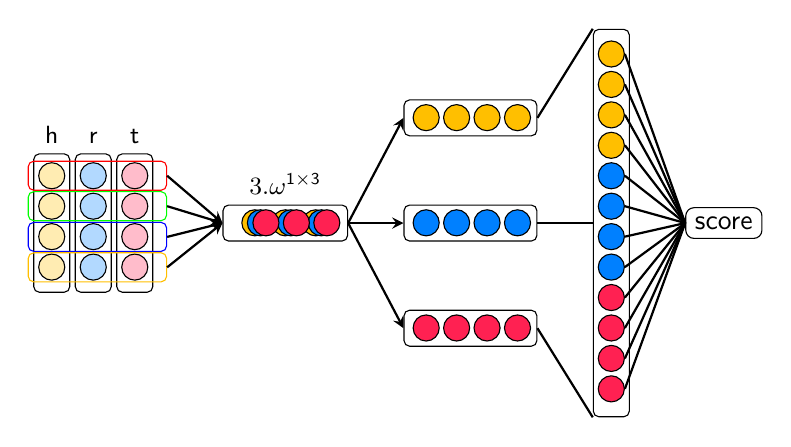
\begin{tikzpicture}[
			emb/.style={draw, circle,minimum width=.1em, thin, anchor=center},
			head/.style={emb, fill=amber},
			relation/.style={emb, fill=azure},
			tail/.style={emb, fill=awesome},
			conv/.style={emb, fill=gray},
			box/.style={draw,rectangle, fill=none},
			embBox/.style={box ,rounded corners=0.2em},
			convBox/.style={box, minimum height=1.3em, minimum width=4.8em,rounded corners=0.2em},
			convolution/.style={box, minimum height=1.3em, minimum width=4.5em,rounded corners=0.2em},
			convLayer/.style={box, minimum height=1.05em, minimum width=5em, rounded corners=0.2em},
			textbox/.style={box,rounded corners=0.3em, fill=none,font=\sffamily, align=center},
			title/.style={fill=none, font=\sffamily, align=center},
			arrow/.style={thick,>=stealth},
			arrowStrong/.style={thick,->,>=stealth},
			arrowStyle/.style={-latex', font=\sffamily},
			mydot/.style={draw, circle, minimum size=0.1em, scale=0.2},
			]
			% 5
			%			\draw node[textbox] (lossConvKB) {$\mathcal{L}\ref{eq:lossConvKB}$};
			\draw node[textbox] (lossConvKB) {score};
			
			\draw node[embBox][minimum width=1.3em, minimum height=14em, left=2em of lossConvKB] (box9) {};
			\foreach \x in {1,...,4}
			{\draw node[head](e9\x)[yshift=-(\x-7)*1.1em, below=0mm of box9.center]{};}
			
			\foreach \x in {1,...,4}
			{\draw node[relation](e8\x)[yshift=(\x-2)*1.1em, below=0mm of box9.center]{};}
			
			\foreach \x in {1,...,4}
			{\draw node[tail](e7\x)[yshift=(\x-6)*1.1em, below=0mm of box9.center]{};}
			
			%
			\draw node[convBox][yshift=3.8em, left=2em of box9] (box6) {};
			\foreach \x in {1,...,4}
			{\draw node[head](e6\x)[yshift=0.5em, xshift=(\x-2)*1.1em-0.5em, below=0mm of box6.center]{};}
			
			\draw node[convBox][left=2em of box9] (box5) {};
			\foreach \x in {1,...,4}
			{\draw node[relation](e5\x)[yshift=0.5em, xshift=(\x-2)*1.1em-0.5em, below=0mm of box5.center]{};}
			
			\draw node[convBox][yshift=-3.8em, left=2em of box9] (box4) {};
			\foreach \x in {1,...,4}
			{\draw node[tail](e4\x)[yshift=0.5em, xshift=(\x-2)*1.1em-0.5em, below=0mm of box4.center]{};}
			
			%
			\draw node[convolution][left=2em of box5] (filterBox1) {};
			\foreach \x in {1,...,3}
			{\draw node[conv, fill=amber](filter1\x)[yshift=0.5em, xshift=(\x-2)*1.1em, below=0mm of filterBox1.center]{};}
			\foreach \x in {1,...,3}
			{\draw node[conv, fill=azure](filter2\x)[yshift=0.5em, xshift=(\x-2)*1.1em+0.2em, below=0mm of filterBox1.center]{};}
			\foreach \x in {1,...,3}
			{\draw node[conv, fill=awesome](filter3\x)[yshift=0.5em, xshift=(\x-2)*1.1em+0.4em, below=0mm of filterBox1.center]{};}
			
			\draw node[embBox][minimum width=1.3em, minimum height=5em, xshift=-1.5em, left=4em of filterBox1] (box1) {};
			\foreach \x in {1,...,4}
			{\draw node[head, fill=amber!30](e1\x)[yshift=(\x-2)*1.1em, below=0mm of box1.center]{};}
			\draw node[title][above=0mm of box1] (headText) {\small $\text{h}$};
			
			\draw node[embBox][minimum width=1.3em, minimum height=5em, left=4em of filterBox1] (box2) {};
			\foreach \x in {1,...,4}
			{\draw node[relation, fill=azure!30](e2\x)[yshift=(\x-2)*1.1em, below=0mm of box2.center]{};}
			\draw node[title][above=0mm of box2] (relationText) {\small $\text{r}$};
			
			\draw node[embBox][minimum width=1.3em, minimum height=5em, xshift=1.5em,left=4em of filterBox1] (box3) {};
			\draw node[title][above=0mm of filterBox1] (filterTitle) {\small $3.\omega^{\text{1} \times \text{3}}$};
			\foreach \x in {1,...,4}
			{\draw node[tail, fill=awesome!30](e3\x)[yshift=(\x-2)*1.1em, below=0mm of box3.center]{};}
			\draw node[title][above=0mm of box3] (tailText) {\small $\text{t}$};
			
			\draw node[convLayer, color=red][yshift=1.71em, left=2em of filterBox1] (conv1){};
			\draw node[convLayer, color=green][yshift=0.61em, left=2em of filterBox1] (conv2){};
			\draw node[convLayer, color=blue][yshift=-0.5em, left=2em of filterBox1] (conv3){};
			\draw node[convLayer, color=amber][yshift=-1.6em, left=2em of filterBox1] (conv4){};
			
			% Arrow
			\foreach \x in {1,...,4}
			\draw [arrowStrong] (conv\x.east) -- (filterBox1.west);
			
			\foreach \x in {4,...,6}
			\draw [arrowStrong] (filterBox1.east) -- (box\x.west);
			
			\draw [arrow] (box4.east) -- (box9.south west);
			\draw [arrow] (box5.east) -- (box9.west);
			\draw [arrow] (box6.east) -- (box9.north west);
			
			\foreach \x in {1,...,4}
			\draw [arrow] (e9\x.east) -- (lossConvKB.west);
			\foreach \x in {1,...,4}
			\draw [arrow] (e8\x.east) -- (lossConvKB.west);
			\foreach \x in {1,...,4}
			\draw [arrow] (e7\x.east) -- (lossConvKB.west);
			
		\end{tikzpicture}
	}
	\caption{Minh họa các lớp giải mã của mô hình ConvKB với 3 filter}
	\label{fig:decoderConvKB}
\end{figure}

Sau khi chúng ta biểu diễn các thực thể và quan hệ lên không gian số chiều thấp, mô hình sẽ sử dụng \cite{nguyen2017novel} làm mô hình để phân tích các đặc trưng toàn cục của một bộ ba $t_{ijk}$ qua mỗi chiều để khái quát hóa các đặc trưng biến đổi của mô hình bằng các lớp tính tích chập. Hàm tính điểm số với những ánh xạ đặc trưng được tính theo công thức sau :

\begin{equation}
	f(t_{i j k}) = \Big( \bigparallel_{m=1}^{\Omega} \text{ReLU} ([\overrightarrow{e_i}, \overrightarrow{r_k}, \overrightarrow{h_j}] \ast \omega^m)\Big).\mathbf{W}
\end{equation}

trong đó $\omega^m$ thể hiện bộ lọc tích chập thứ $m-th$,
\(\omega\) là siêu tham số về số lượng lớp tích chập, \(\ast\) là thao tác thực hiện tính tích chập, và \(\mathbf{W} \in \mathbb{R}^{\Omega k \times 1}\)
biểu thị ma trận biến đổi tuyến tính được sử dụng để tính kết quả cuối cùng của bộ ba. Mô hình được huấn luyện bằng lề-mềm (soft-margin) như sau :

\begin{equation}
	\label{eq:lossConvKB}
	\mathcal{L} = \sum_{t^k_{ij} \in \{S \cup S'\}} \text{log}(1 + exp(l_{t^k_{ij}} . f(t^k_{ij}))) + \frac{\lambda}{2} \parallel{\mathbf{W}}\parallel_2^2
\end{equation}
trong đó $l_{t^k_{ij}} = \begin{cases}
	1 &\text{for } t^k_{ij} \in S \\
	-1 &\text{for } t^k_{ij} \in S' \\
\end{cases}$

Đầu ra cuối cùng của mô hình ConvKB là điểm số xếp hạng của từng dự đoán.


% % Phương pháp đề xuất
% \chapter{Phương pháp đề xuất}

% Phương pháp đề xuất dựa trên luất
\section{AnyBURL}

Anytime Bottom-Up Rule Learning for Knowledge Graph Completion \cite{meilicke2019anytime}
sdfsdf

% Phương pháp đề xuất dựa trên học sâu
\section{Mô hình GCAT}
\label{sec:GCAT}

% Kết quả thí nghiệm
%\chapter{EXPERIMENTS}
%\label{Chapter4}

%\chapter{Thực nghiệm}
\chapter{EXPERIMENTS}
\label{chap:Experiment}

%\begin{center}
%\begin{tikzpicture}
%	[every axis/.style={
	%		ybar,
	%		scale only axis,
	%		ymin=0, ymax= 50000,
	%		width=0.5\textwidth,
	%		height=0.4\textwidth,
	%		legend style={at={(20em,5em)}, anchor=east},
	%		bar width=1em,
	%		scaled y ticks=false,
	%		xtick=data,
	%		font=\scriptsize\sffamily,
	%		symbolic x coords={Dataset,FB15k,FB15k-237,WN18,WN18RR},
	%		nodes near coords,
	%		nodes near coords align={vertical},
	%	}]
%	\pgfplotsset{
	%		compat=newest,
	%		major grid style=blue,
	%		xlabel near ticks,
	%		ylabel near ticks
	%	}
%	
%	\begin{axis}[]
	%		\addplot [fill=awesome] coordinates {
		%			(FB15k,14951)
		%			(FB15k-237,14541)
		%			(WN18,40943)
		%			(WN18RR,40559)
		%			(YAGO3-10, 123182)
		%		};
	%		\addplot [fill=azure] coordinates {
		%			(FB15k,1345)
		%			(FB15k-237,237)
		%			(WN18,18)
		%			(WN18RR,11)
		%			(YAGO3-10,37)
		%		};
	%		\legend{Entities, Relations}
	%	\end{axis}
%\end{tikzpicture}
%\end{center}

\begin{figure}[h]
	\centering
		\label{fig:dataset}
		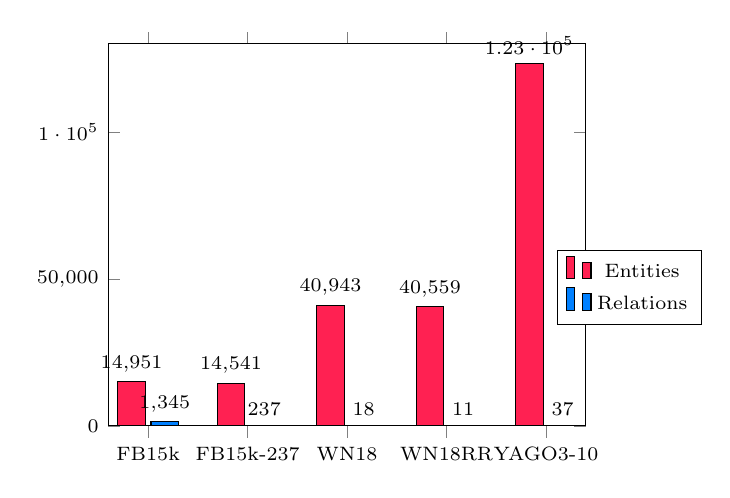
\begin{tikzpicture}
			[every axis/.style={
				ybar,
				scale only axis,
				ymin=0, ymax= 130000,
				width=0.5\textwidth,
				height=0.4\textwidth,
				legend style={at={(20em,5em)}, anchor=east},
				bar width=1em,
				scaled y ticks=false,
				xtick=data,
				font=\scriptsize,
				symbolic x coords={FB15k,FB15k-237,WN18,WN18RR,YAGO3-10},
				nodes near coords,
				nodes near coords align={vertical},
			}]
			\pgfplotsset{
				compat=newest,
				major grid style=blue,
				xlabel near ticks,
				ylabel near ticks
			}
			
			\begin{axis}[]
				\addplot [fill=awesome] coordinates {
					(FB15k,14951)
					(FB15k-237,14541)
					(WN18,40943)
					(WN18RR,40559)
					(YAGO3-10,123182)
				};
				\addplot [fill=azure] coordinates {
					(FB15k,1345)
					(FB15k-237,237)
					(WN18,18)
					(WN18RR,11)
					(YAGO3-10,37)
				};
				\legend{Entities, Relations}
			\end{axis}
		\end{tikzpicture}
	
\end{figure}


In this section, we describe the datasets used for our empirical evaluation, along with a comparison against notable existing methods as reported in \autoref{tab:graphEmbeddingTechCompare}. Additionally, we evaluate our two proposed approaches for injecting new knowledge into the knowledge graph. Specifically, we treat the test set as a batch of new knowledge to be added, and use the validation set to re-evaluate the effectiveness of our method. Detailed results are presented in \autoref{tab:resultOnFreeBase} and \autoref{tab:resultOnWordNet}.


\begin{table}[H]
	\begin{center}
%		\resizebox{\textwidth}{!}{%
			\begin{tabular}{llllll}
				\hline
				&          &           & \multicolumn{3}{l}{\# Edges}    \\ \cline{4-6}
				
				Dataset   & Entities & Relations & Training & Validation & Test    \\ \hline
				FB15k     & 14,951   & 1,345     & 483,142  & 50,000     & 59,071 \\
				FB15k-237 & 14,541   & 237       & 272,115  & 17,535     & 20,466  \\
				WN18      & 40,943   & 18        & 141,442  & 5,000      & 5,000   \\
				WN18RR    & 40,559   & 11        & 86,835   & 3,034       & 3,134    \\
				YAGO3-10    & 123,182   & 37        & 1,079,040   & 5,000       & 5,000  \\
				\hline
			\end{tabular}
%		}
		\caption{Dataset Information}
		\label{tab:datasetInfo}
	\end{center}
\end{table}

%\section{Các tập dữ liệu huấn luyện}
\section{Training Datasets}
\label{sec:DataTraining}

\begin{figure}[H]
	\centering
	\label{fig:dataset_split}
\pgfplotstableread[row sep=\\,col sep=&]{
	Dataset & Entities & Relations & Training & Validation & Test\\
	FB15k & 14951 & 1345 & 483142 & 50000 & 59071  \\
	FB15k-237 & 14541 & 237 & 272115 & 17535 & 20466  \\
	WN18 & 40943 & 18 & 141442 & 5000 & 5000  \\
	WN18RR & 40559 & 11 & 86835 & 3034 & 3134  \\
	YAGO3-10 & 123182 & 37 & 1079040 & 5000 & 5000  \\
}\mydata
\resizebox{\textwidth}{!}{%
	\begin{tikzpicture}
		\begin{axis}[
			xbar stacked,
			tick align = outside, xtick pos = left,
			scale only axis,
			scaled x ticks=false,
			every node near coord/.style={/pgf/number format/fixed},
			xticklabel style={/pgf/number format/fixed},
			width=\textwidth,
			height=0.3\textwidth,
			font=\scriptsize,
			legend style={at={(0.5,-0.15)}, anchor=north, legend columns=-1},
			bar width=1.5em,
			ytick=data,
			y dir = reverse,
			yticklabels from table={\mydata}{Dataset},
			]
			\addplot[fill=azure] table [y expr=\coordindex,x=Training]{\mydata};
			\addplot+[fill=awesome] table [y expr=\coordindex,x=Validation]{\mydata};
			\addplot+[fill=amber,
			point meta=x,
			nodes near coords = {\pgfmathprintnumber[precision=1]{\pgfplotspointmeta}},
			nodes near coords align={anchor=west},
			every node near coord/.append style={
				black,
				fill=white,
				fill opacity=0.75,
				text opacity=1,
				outer sep=\pgflinewidth
			}] table [y expr=\coordindex,x=Test]{\mydata};
			\legend{Training, Validation, Test};
		\end{axis}
	\end{tikzpicture}
}
\end{figure}


In our experiments, we evaluate our approach on four widely used benchmark datasets: FB15k, FB15k-237 (\cite{toutanova2015observed}), WN18, and WN18RR (\cite{dettmers2018convolutional}). Each dataset is divided into three subsets: training, validation, and test sets. Detailed statistics for these datasets are presented in \autoref{tab:datasetInfo}. 

Each dataset consists of a collection of triples in the form \(\langle head, relation, tail \rangle\). FB15k and WN18 are derived from the larger knowledge bases FreeBase and WordNet, respectively. However, they contain a large number of inverse relations, which allow most triples to be easily inferred. To address this issue and to better reflect real-world link prediction scenarios, FB15k-237 and WN18RR were constructed by removing such inverse relations.

\subsection{FB15k Dataset}

This dataset was constructed by the research group of A. Bordes and N. Usunier \cite{bordes2013translating} by extracting data from the Wikilinks database\footnote{https://code.google.com/archive/p/wiki-links/}. The Wikilinks database contains hyperlinks to Wikipedia articles, comprising over 40 million mentions of approximately 3 million entities. The authors extracted all facts related to a given entity that is mentioned at least 100 times across different documents, along with all facts associated with those entities (including child entities mentioned in the corresponding Wikipedia articles), excluding attributes such as dates, proper nouns, etc. 

Entities with degree \(n\) were normalized by converting multi-way edges into sets of binary relations—enumerating all edges and relations between each pair of nodes.

%\ The dataset is randomly split into three subsets: the training set includes 1345 relations, 14,834 head entities, and 14,903 tail entities; the test set includes 916 relations, 11,886 head entities, and 11,285 tail entities; and the validation set includes 961 relations, 12,297 head entities, and 11,825 tail entities.

\subsection{FB15k-237 Dataset}

This dataset is a subset of FB15k, constructed by Toutanova and Chen \cite{toutanova2015observed}, motivated by the observation that FB15k suffers from test leakage, where models are exposed to test facts during training. This issue arises due to the presence of duplicate or inverse relations in FB15k. FB15k-237 was created to provide a more challenging benchmark. The authors selected facts related to the 401 most frequent relations and eliminated all redundant or inverse relations. Additionally, they ensured that no entities connected in the training set were directly linked in the test and validation sets.

%\ The training set includes 237 relations, 13,781 head entities, and 13,379 tail entities; the test set includes 223 relations, 7,652 head entities, and 5,804 tail entities; and the validation set includes 224 relations, 8,171 head entities, and 6,376 tail entities.



\subsection{WN18 Dataset}

\begin{center}
	\resizebox{\textwidth}{!}{%
		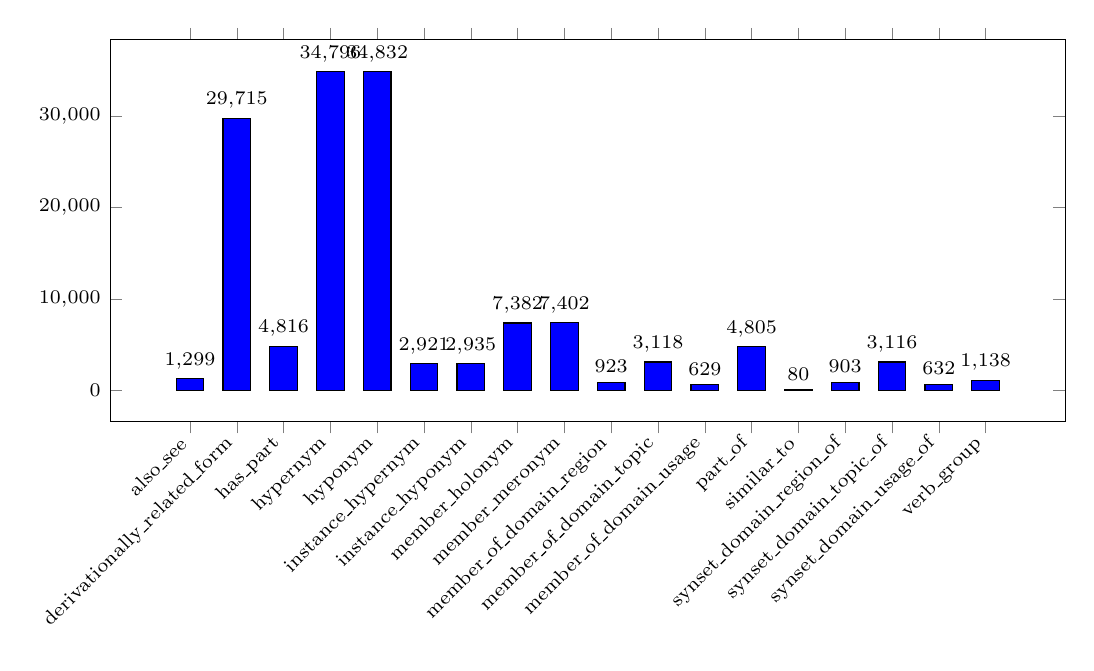
\begin{tikzpicture}
			[every axis/.style={
				ybar,
				scale only axis,
				width=\textwidth,
				height=0.4\textwidth,
				xtick=data,
				x tick label style={rotate=45, anchor=east},
				legend style={at={(20em,5em)}, anchor=east},
				bar width=1em,
				scaled y ticks=false,
				font=\scriptsize,
				symbolic x coords={
					also\_see,
					derivationally\_related\_form,
					has\_part,
					hypernym,
					hyponym,
					instance\_hypernym,
					instance\_hyponym,
					member\_holonym,
					member\_meronym,
					member\_of\_domain\_region,
					member\_of\_domain\_topic,
					member\_of\_domain\_usage,
					part\_of,
					similar\_to,
					synset\_domain\_region\_of,
					synset\_domain\_topic\_of,
					synset\_domain\_usage\_of,
					verb\_group},
				nodes near coords,
				nodes near coords align={vertical},
			}]
			\pgfplotsset{
				compat=newest,
				major grid style=blue,
				xlabel near ticks,
				ylabel near ticks
			}
			
			\begin{axis}[]
				\addplot [fill=blue] coordinates {
					(also\_see,1299)
					(derivationally\_related\_form,29715)
					(has\_part,4816)
					(hypernym,34796)
					(hyponym,34832)
					(instance\_hypernym,2921)
					(instance\_hyponym,2935)
					(member\_holonym,7382)
					(member\_meronym,7402)
					(member\_of\_domain\_region,923)
					(member\_of\_domain\_topic,3118)
					(member\_of\_domain\_usage,629)
					(part\_of,4805)
					(similar\_to,80)
					(synset\_domain\_region\_of,903)
					(synset\_domain\_topic\_of,3116)
					(synset\_domain\_usage\_of,632)
					(verb\_group,1138)
				};
			\end{axis}
		\end{tikzpicture}
	}
\end{center}

This dataset was introduced by the authors of TransE \cite{bordes2013translating}, and is extracted from WordNet\footnote{https://wordnet.princeton.edu/}, a lexical knowledge graph ontology designed to provide a dictionary/thesaurus to support NLP tasks and automated text analysis. In WordNet, entities correspond to synsets (i.e., \textit{word senses}), and relations represent lexical connections among them (e.g., “hypernym”). 

To construct WN18, the authors used WordNet as a starting point and iteratively filtered out entities and relations that were infrequently mentioned.


%Tập dữ liệu được chia ngẫu nhiên thành 3 tập: tập training với 18 relations, 40504 head entities, và 40551 tail entities, tập test gồm 18 relations, 4262 head entities, and 4338 tail entities, tập vadiation gồm 18 relations, 4349 head entities, and 4263 tail entities.

\subsection{WN18RR Dataset}

This dataset is a subset of WN18, constructed by DeŠmers et al.\cite{dettmers2017convolutional}, who also addressed the issue of test leakage in WN18. To tackle this issue, they created the WN18RR dataset, which is significantly more challenging, by applying a similar methodology to that used in FB15k-237 \cite{toutanova2015observed}.

\section{Evaluation Metrics}

In this section, we describe the evaluation metrics, experimental environment, and datasets used to assess the proposed method. These metrics are widely adopted for evaluating link prediction models on knowledge graphs. We compare our approach against four other state-of-the-art methods reported in \cite{rossi2020knowledge}.

\subsubsection{Hits@K (H@K)}

This metric measures the proportion of correct predictions whose rank is less than or equal to the threshold \(K\):
\[
H@K = \frac{\mid \{ q \in Q : \text{rank}(q) \leq K \} \mid}{\mid Q \mid}
\]

\subsubsection{Mean Rank (MR)}

This metric calculates the average rank of the correct entity in the prediction. A lower value indicates better model performance:
\[
MR = \frac{1}{\mid Q \mid} \sum_{q \in Q} \text{rank}(q)
\]
Here, \(\mid Q \mid\) denotes the total number of queries, which equals the size of the test or validation set. During evaluation, we perform both head and tail entity predictions for each triple. For example, we predict both \(\langle ?,~ \text{relation},~ \text{tail} \rangle\) and \(\langle \text{head},~ \text{relation},~ ? \rangle\). The variable \(q\) denotes a query, and \(\text{rank}(q)\) indicates the rank position of the correct entity. The final MR score is the average rank over all head and tail predictions.

Clearly, this metric ranges from \([1,~|\text{number of entities}|]\), as a node can connect to at most \(n-1\) other nodes plus a self-loop. However, this metric is highly sensitive to outliers, as certain relations may yield extremely low rankings for correct entities. To address this issue, our method—as well as other recent works—also adopts the Mean Reciprocal Rank (MRR) metric.


\subsubsection{Mean Reciprocal Rank (MMR)}
This is the Mean Reciprocal Rank (MRR), calculated as the reciprocal of the average rank obtained for a correct prediction. Higher values indicate better model performance. Since this metric takes the reciprocal of each rank, it helps mitigate the noise sensitivity encountered in the Mean Rank (MR) metric:
\[
MRR =\frac{1}{\mid Q \mid} \sum_{q \in Q} \frac{1}{\text{rank}(q)}
\]

\section{Training Methodology}

%\subsection{Training with the AnyBURL Model}

\subsection{Training with the KBGAT Model}

We first initialize the entity and relation embeddings using the TransE model \cite{bordes2013translating}. To construct negative (invalid) triples, we randomly replace either the head or tail entity in a valid triple with another entity sampled from the entity set.

The training process is divided into two phases. The first phase serves as an encoder, transforming the initialized embeddings into new embeddings that aggregate neighborhood information using the KBGAT model. This produces updated embeddings for both entities and relations. The second phase serves as a decoder, performing link prediction by incorporating $n$-hop neighborhood information. This enables the model to better aggregate context from neighboring entities. Furthermore, we incorporate auxiliary relations to enrich the local structure in sparse graphs.

We use the Adam optimizer with a learning rate of $\mu = 0.001$. The final embedding dimension for both entities and relations is set to 200. The optimal hyperparameters are determined via grid search, as detailed in \autoref{appendix:Appendix1}.


\section{Experimental Results}
\label{sec:Experiment}

As previously mentioned, our rule-based model can be fully executed on a standard laptop. In our experiment, the machine configuration was as follows: T480, Core i5 8th Gen, 16GB RAM, 4 cores and 8 threads. The source code was implemented in Python version 3.6, utilizing only built-in Python functions without any third-party libraries. The experiments were conducted on four widely-used datasets: FB15k, FB15-237, WN18, and WN18RR. Detailed information about these datasets is provided in \autoref{sec:DataTraining} under the training datasets section.

As described in \autoref{alg:GenerateRules}, the AnyBURL algorithm learns rules generated within a user-configurable time interval. Here, we set the training time to 1000 seconds (approximately 17 minutes), with saturation (SAT) set to \(0.85\), confidence threshold Q set to \(0.05\), and sample size S configured as (\(\frac{1}{10}~ \text{of the training set}\)). With this setup, our Python version of the model produced results comparable to the Java version developed by Meilicke, Christian et al. \cite{burl}, which was configured similarly but trained for only 100 seconds. The difference in training time is primarily due to performance differences between Python and Java. We chose Python because it is the primary language used in many recent artificial intelligence models and provides convenience for performance comparison and evaluation with other deep learning methods, most of which are also implemented in Python.



\begin{table}[H]
	\begin{center}
		\caption{Experimental results on the FB15k and FB15k-237 datasets}
		\label{tab:resultOnFreeBase}%
		\resizebox{0.9\textwidth}{!}{%
			\begin{tabular}{l|l|l|l|l|l|l|l|l|}
				\cline{2-9}
				& \multicolumn{4}{c|}{\textbf{FB15k}}                   & \multicolumn{4}{c|}{\textbf{FB15k-237}}                   \\ \cline{2-9} 
				& \textbf{H@1} & \textbf{H@10} & \textbf{MR} & \textbf{MRR} & \textbf{H@1} & \textbf{H@10} & \textbf{MR} & \textbf{MRR} \\ \hline
				\multicolumn{1}{|l|}{ComplEx} & 81.56        & 90.53         & 34          & 0.848        & 25.72        & 52.97         & 202        & 0.349        \\ \hline
				\multicolumn{1}{|l|}{TuckER}  & 72.89        & 88.88         & 39          & 0.788        & 25.90        & 53.61         & 162         & 0.352        \\ \hline
				\multicolumn{1}{|l|}{TransE}  & 49.36        & 84.73         & 45          & 0.628        & 21.72        & 49.65         & 209         & 0.31        \\ \hline
				\multicolumn{1}{|l|}{RoteE}   & 73.93        & 88.10         & 42          & 0.791        & 23.83        & 53.06         & 178         & 0.336        \\ \hline
				\multicolumn{1}{|l|}{ConvKB}  & 59.46        & 84.94         & 51         & 0.688        & 21.90        & 47.62         & 281         &0.305        \\ \hline
				\multicolumn{1}{|l|}{\textbf{KBGAT}}     &  70.08            &     91.64    &  38    &   0.784    & 36.06     &    58.32   &  211  &    0.4353  \\ \hline
				\multicolumn{1}{|l|}{\textbf{AnyBURL}}    & 79.13        & 82.30         & 285         & \underline{0.824}        & 20.85        & 42.40         & 490         & 0.311        \\ \hline
			\end{tabular}
		}
	\end{center}
\end{table}


\begin{table}[H]
	\begin{center}
		\caption{Experimental results on the WN18 and WN18RR datasets}
		\label{tab:resultOnWordNet}%
		\resizebox{0.9\textwidth}{!}{%
			\begin{tabular}{l|l|l|l|l|l|l|l|l|}
				\cline{2-9}
				& \multicolumn{4}{c|}{\textbf{WN18}}                              & \multicolumn{4}{c|}{\textbf{WN18RR}}                            \\ \cline{2-9} 
				& \textbf{H@1}   & \textbf{H@10}  & \textbf{MR}  & \textbf{MRR}   & \textbf{H@1}   & \textbf{H@10}  & \textbf{MR}  & \textbf{MRR}   \\ \hline
				\multicolumn{1}{|l|}{ComplEx} & 94.53          & 95.50          & 3623         & 0.349          & 42.55          & 52.12          & 4909         & 0.458          \\ \hline
				\multicolumn{1}{|l|}{TuckER}  & 94.64          & 95.80          & 510          & 0.951          & 42.95          & 51.40          & 6239         & 0.459          \\ \hline
				\multicolumn{1}{|l|}{TransE}  & 40.56          & 94.87          & 279          & 0.646          & 2.79           & 94.87          & 279          & 0.646          \\ \hline
				\multicolumn{1}{|l|}{RoteE}   & 94.30          & 96.02          & 274          & 0.949          & 42.60          & 57.35          & 3318         & 0.475          \\ \hline
				\multicolumn{1}{|l|}{ConvKB}  & 93.89          & 95.68          & 413          & 0.945          & 38.99          & 50.75          & 4944         & 0.427          \\ \hline
				\multicolumn{1}{|l|}{\textbf{KBGAT}}     &                &        &        &                &       35.12         &        57.01         &      \underline{1974}       &  0.4301           \\ \hline
				\multicolumn{1}{|l|}{\textbf{AnyBURL}}    &  93.96 & 95.07 & \textbf{230} & \textbf{0.955} & \textbf{44.22} & 54.40 & 2533 & \underline{0.497} \\ \hline
			\end{tabular}
		}
	\end{center}
\end{table}


\autoref{tab:resultOnFreeBase} and \autoref{tab:resultOnWordNet} describe our experimental results with the \(H@K\) metrics along with the experimental results of other methods mentioned in the survey \cite{rossi2020knowledge}.


\begin{table}[H]
	\begin{center}
		\caption{Accuracy results of the two new knowledge addition strategies}
		\label{tab:CompareAccuracy}%
		\resizebox{0.8\columnwidth}{!}{%
			\begin{tabular}{ll|l|l|l|}
				\cline{3-5}
				&        & \textbf{AnyBURL} & \textbf{Batch edge AnyBURL} & \textbf{Edge AnyBURL} \\ \hline
				\multicolumn{1}{|l|}{\multirow{3}{*}{\textbf{FB-15k}}}    & hit@10 & 82.22                  & 82.48               & 83.08               \\ \cline{2-5} 
				\multicolumn{1}{|l|}{}                                    & MR     & 285                    & 250                 & 220                 \\ \cline{2-5} 
				\multicolumn{1}{|l|}{}                                    & MRR    & 0.824                  & 0.853               & 0.866               \\ \hline
				\multicolumn{1}{|l|}{\multirow{3}{*}{\textbf{FB15k-237}}} & hit@10 & 42.40                  & 43.40               & 43.51               \\ \cline{2-5} 
				\multicolumn{1}{|l|}{}                                    & MR     & 490                    & 472                 & 441                 \\ \cline{2-5} 
				\multicolumn{1}{|l|}{}                                    & MRR    & 0.311                  & 0.353               & 0.377               \\ \hline
				\multicolumn{1}{|l|}{\multirow{3}{*}{\textbf{WN18}}}      & hit@10 & 95.07                  & 95.09               & 95.19               \\ \cline{2-5} 
				\multicolumn{1}{|l|}{}                                    & MR     & 230                    & 229                 & 228                 \\ \cline{2-5} 
				\multicolumn{1}{|l|}{}                                    & MRR    & 0.955                  & 0.955               & 0.956               \\ \hline
				\multicolumn{1}{|l|}{\multirow{3}{*}{\textbf{WN18RR}}}    & hit@10 & 54.40                  & 54.63               & 54.70               \\ \cline{2-5} 
				\multicolumn{1}{|l|}{}                                    & MR     & 2533                   & 2346                & 2215                \\ \cline{2-5} 
				\multicolumn{1}{|l|}{}                                    & MRR    & 0.497                  & 0.553               & 0.581               \\ \hline
			\end{tabular}
		}
	\end{center}
\end{table}

\autoref{tab:CompareAccuracy} describes our experimental results for the two strategies of adding new knowledge into the graph. We evaluate the total number of generated rules, as well as the number of rules with confidence \(>= 50\%\) and \(>= 80\%\).

\begin{table}[H]
	\begin{center}
		\caption{Evaluation results on the number of rules of the two new knowledge addition strategies}
		\label{tab:CompareRule}%
		\resizebox{0.8\columnwidth}{!}{%
			\begin{tabular}{ll|l|l|}
				\cline{3-4}
				& & \textbf{Batch edge AnyBURL} & \textbf{Edge AnyBURL}  \\ \hline
				\multicolumn{1}{|c|}{\multirow{3}{*}{\textbf{FB15k}}}     & num rule        & 1011                       & 1367                      \\ \cline{2-4} 
				\multicolumn{1}{|c|}{}& confidence 50\% & 416 (41,14\%)              & 1185 (86,69\%)            \\ \cline{2-4} 
				\multicolumn{1}{|c|}{}& confidence 80\% & 284 (28, 09\%)             & 481 (35,18\%)             \\ \hline
				\multicolumn{1}{|l|}{\multirow{3}{*}{\textbf{FB15k-237}}} & num rule        & 1120                       & 756                       \\ \cline{2-4} 
				\multicolumn{1}{|l|}{}& confidence 50\% & 244 (21,79\%)              & 660 (87,30\%)             \\ \cline{2-4} 
				\multicolumn{1}{|l|}{}& confidence 80\% & 95 (8,48\%)                & 162 (21,43\%)             \\ \hline
				\multicolumn{1}{|l|}{\multirow{3}{*}{\textbf{WN18}}}      & num rule        & 533                        & 260                       \\ \cline{2-4} 
				\multicolumn{1}{|l|}{}& confidence 50\% & 270 (38, 46 \%)            & 252 (96,92\%)             \\ \cline{2-4} 
				\multicolumn{1}{|l|}{}& confidence 80\% & 240 (34,19\%)              & 225 (86,54\%)             \\ \hline
				\multicolumn{1}{|l|}{\multirow{3}{*}{\textbf{WN18RR}}}    & num rule        & 439                        & 106                       \\ \cline{2-4} 
				\multicolumn{1}{|l|}{}& confidence 50\% & 110 (25,05\%)              & 102 (96,22\%)             \\ \cline{2-4} 
				\multicolumn{1}{|l|}{}& confidence 80\% & 83 (18,91\%)               & 85 (81,19\%)              \\ \hline
			\end{tabular}
		}
	\end{center}
\end{table}


% Kêt luận
\chapter{Kết luận}
\label{chap:Conclusion}

Trong phần này chúng tôi sẽ trình bày các kết quả đạt được của mô hình chúng tôi, cũng như những phân tích của chúng tôi
trên các kết quả của các tập dữ liệu khác nhau để giải thích những điểm tốt và điểm cần cải thiện trên mô hình của chúng tôi trên tập dữ liệu đó. Từ đó chúng tôi xác định những hướng nghiên cứu để cải tiến trong tương lai.
% chúng tôi cố gắng tìm hiểu các đặc trưng của các bộ dữ liệu tương ứng để cố gắng lý  giải thích  tại sao mô hình của chúng tôi hoặc các công trình khác có được kết quả tốt trên tập dữ liệu tương ứng đó.
% Những kết quả của hai đề xuất của chúng tôi cũng như các dịnh hướng nghiên cứu của chúng tôi trong tương lai.

Mặc dù kết quả chúng tôi cho thấy phương pháp dựa trên luật của chúng tôi có hiệu suất tương đương với các mô hình học sâu hiện đại (state-of-art) và có ưu thế vượt trội trong thời gian đào tạo khoảng 17 phút so với thời gian hàng giờ của phương pháp học sâu khác nhưng không phải là các mô hình học sâu này không đáng nghiên cứu. Chúng tôi cũng nhận thấy, với tập dữ liệu có nhiều loại quan hệ khác nhau như FreeBase, mô hình GCAT nhờ sử dụng cơ chế chú ý đạt được kết quả tốt hơn so với tập WorldNet với số lượng các loại quan hệ ít hơn.
Điều này chứng tỏ cơ chế chú ý bổ sung thêm thông tin vector nhúng quan hệ giúp học được các cấu trúc của đồ thị tốt hơn trên các tập dữ liệu nhiều loại quan hệ.
Đối với tập dữ liệu có nhiều mẫu tương tự và nghịch đảo như FB15k và WN18RR, mô hình dựa trên luật AnyBURL đạt được kết quả vượt trội, trong khi với phương pháp học sâu mô hình chỉ đạt kết quả trung bình so với các phương pháp khác.
Mô hình dựa trên luật AnyBURL có ưu thế tốt hơn trên các tập dữ liệu FB15k và WN18RR, tuy nhiên với các tập dữ liệu đã loại bỏ các thông tin tương tự hoặc nghịch đảo như FB15-237 và WN18RR thì phương pháp dựa trên luật tỏ ra kém hiệu quả hơn vì mô hình này học dựa trên các đường đi hoặc liên kết đã xảy ra. Với phương pháp học sâu, mô hình biểu diễn các quan hệ và thực thể lên không gian để học được mối quan hệ giữa chúng, chính vì vậy mà mô hình học sâu đạt kết quả tốt hơn trên các tập dữ liệu như FB15k-237 và WN18RR so với các tập dữ liệu như FB15k và WN18.
Một trong những ưu điểm của phương pháp dựa trên luật đó là các luật được sinh ra có thể lý giải được trong quá trình học, và có thời gian học vượt trội so với các phương pháp khác. Tuy nhiên, sau quá trình học phương pháp dựa trên luật phải duyệt qua tất cả các luật đã học mới có thể đưa ra được dự đoán. Đây là một điểm mà các phương pháp học sâu thể hiện tốt hơn, vì thông qua các trọng số đã học, mô hình học sâu GCAT thông qua các lớp tính toán có thể biến đổi đầu vào thành các kết quả xác xuất dự đoán nhanh hơn. Nhược điểm với phương pháp học sâu là quá trình học không thể lý giải được, hơn nữa chí phí huấn luyện rất tốn kém. Đối với hai thuật toán mở rộng của chúng tôi trong việc thêm tri thức mới vào đồ thị chúng tôi nhận thấy rằng là vượt trội hoàn toàn so với các phương pháp học sâu.
% Ngược lại đối với các phương pháp dựa trên học sâu lại có ưu thế rất lớn trong các tập dữ liệu này do có thể dễ dàng tính toán độ gần của các luật mới cần đánh giá so với các luật đã học từ đó có một kết quả khá tốt.
% Do đó chúng tôi cũng sẽ tiếp tục nghiên cứu các phương pháp học sâu và sẽ dùng phương pháp này làm đường cơ sở (base line) để so sánh với các nghiên cứu của chúng tôi trong tương lai.
% Một điểm yếu nữa của mô hình đựa trên luật của chúng tôi là mặc dù thời gian học là vượt trội nhưng thời gian để tính toán đưa ra đự đoán khá lâu do phải duyệt qua tất cả các luật được sinh ra mới có thể đưa ra dự đoán.
% Không giống như các phương pháp nhúng đồ thị khác thao tác này có thể dễ dàng tính toán.

Quá trình nhúng đồ thị giúp biểu diễn các đặc trưng của thực thể, quan hệ hay các đặc trưng của đồ thị tri thức thành các vector có số chiều thấp hơn (\ref{sec:graphEmbedding}), nhưng trong thực tế, một tri thức được biểu diễn bằng những thực thể và những quan hệ là hoàn toàn độc lập với nhau nên cần phải biểu diễn chúng thành các vector có số chiều khác nhau, tỷ lệ số chiều giữa chúng cũng là vấn đề quan trọng cần nghiên cứu. Bên cạnh đó, trong thế giới thực, yếu tố thời gian là thông tin quan trọng có thể thay đổi hoàn toàn ý nghĩa của một tri thức. Vì vậy, cách cơ chế chú ý bổ sung thêm thông tin thời gian là một trong những hướng nghiên cứu chúng tôi cần áp dụng để đảm bảo tính đúng đắn của đồ thị tri thức. Đối với phương pháp học trên luật AnyBURL, gần đây nhánh học tăng cường (reinforcement learning) khá phát triển và nhóm tác giả Meilicke, Christian and Chekol \cite{meilicke2020reinforced} gần đây cũng đã có 1 nghiên cứu để tối ưu hóa lại phương pháp AnyBURL này.
Chúng tôi cũng có ý định nghiên cứu về hướng này và cố gắng báo cáo lại trong một tương lai không xa.

% Công trình của tác giả (nếu không có thì comment 02 dòng dưới)
% \addcontentsline{toc}{chapter}{Danh mục công trình của tác giả}
% \chapter*{Danh mục công trình của tác giả}
\label{Publish}

\begin{enumerate}
\item Tạp chí ABC
\item Tạp chí XYZ
\end{enumerate}

% In tài liệu tham khảo
\addcontentsline{toc}{chapter}{Tài liệu tham khảo}
\printbibheading[title={Tài liệu tham khảo}]

\printbibliography[heading=subbibliography, title={Tiếng Việt}, keyword=Viet, resetnumbers=true]

\DeclareNameAlias{sortname}{last-first}
\DeclareNameAlias{default}{last-first}

\printbibliography[heading=subbibliography, title={Tiếng Anh}, notkeyword=Viet, resetnumbers=2]
% ===================================================================== %
% CHÚ Ý: phải gán lại resetnumbers=số tài liệu tham khảo tiếng Việt + 1 %
% ===================================================================== %

% Phần phụ lục
\appendix 

\chapter{Các siêu tham số tối ưu}
\label{Appendix1}

Trong phần này chúng tôi sẽ báo cáo lại tập hợp các siêu tham số tối ưu trên cả mô hình Chú ý và mô hình ConvKB.
Chúng tôi sử dụng tìm kiếm lưới theo Hits@10 để tìm các tham số tối ưu. Chúng tôi không chia nhỏ tập dữ liệu trong quá trình huấn luyện mô hình chú ý,
đối với mô hình dự đoán, chúng tôi sử dụng kích thước cho tất cả các tập dữ liệu. Cụ thể các siêu tham số chúng tôi sử dụng được trình bày trong bảng sau :

\begin{table}[htbp]
	\begin{center}
		\resizebox{\textwidth}{!}{%
	\begin{tabular}{llllllllll}
		\hline
		& $\mu$  & Weight decay & Epochs & negative ratio  & Dropouts  & $\alpha_{\text{LeakyRELU}}$ & $N_{\text{head}}$ & $D_{\text{final}}$ & $\gamma$ \\
		\hline
		FB15k     & 1e-3 & 1e-5 & 3000 & 2 & 0.3 & 0.2 & 2 & 200 & 1 \\
		FB15k-237 & 1e-3 & 1e-5 & 3000 & 2 & 0.3 & 0.2 & 2 & 200 & 1 \\
		WN18      & 1e-3 & 5e-6 & 3600 & 2 & 0.3 & 0.2 & 2 & 200 & 5 \\
		WN18RR    & 1e-3 & 5e-6 & 3600 & 2 & 0.3 & 0.2 & 2 & 200 & 5 \\
		\hline
	\end{tabular}
}
\end{center}
\end{table}
% \chapter{Bảng thuật ngữ}
\label{Appendix2}

\printglossary[type=\acronymtype]

\end{document} 